%\documentclass[a4paper]{book}
\documentclass[
a4paper, % Stock and paper size.
12pt, % Type size.
% article,
% oneside, 
onecolumn, % Only one column of text on a page.
openright, % Each chapter will start on a recto page.
% openleft, % Each chapter will start on a verso page.
%openany, % A chapter may start on either a recto or verso page.
]{memoir}

\usepackage[slovene]{babel}
%\usepackage[cp1250]{inputenc}
\usepackage[utf8]{inputenc}
\usepackage[T1]{fontenc}
\usepackage{graphicx}
\usepackage{amsmath,amssymb,mathtools} % Math
\usepackage{multirow}
\usepackage{alltt}
\usepackage[normalem]{ulem}
\usepackage{color}
\usepackage{appendix}
\usepackage{tikz}
\usepackage[final]{microtype} % Less badboxes
\usepackage{lmodern}

%\usepackage{amsthm}
\usepackage{color}

\usepackage{listings}

%\DeclareRobustCommand{\hsout}[1]{\texorpdfstring{\sout{#1}}{#1}}

\newcommand{\hsout}[1]{\ifmmode\text{\sout{\ensuremath{#1}}}\else\sout{#1}\fi}

\newcommand{\red}[1]{\textcolor{red}{#1}}

\usepackage{tikz}



\usepackage{rotating}
\newcommand\rottext[1]{\rotatebox{90}{\parbox{2cm}{\centering#1}}}

\usepackage{epstopdf}

\graphicspath{{img/}}


\input{kvmacros.tex}

%\newcommand{\red}[1]{\textcolor{red}{#1}}

\setlength{\parindent}{0in}
\newcommand{\ol}{\overline}
\newcommand{\sh}{\uparrow}
\newcommand{\pc}{\downarrow}
\newcommand{\imp}{\rightarrow}

\newtheorem{zgled}{Zgled}
\newtheorem{resitev}{Rešitev}
\newcommand{\angl}[1]{(angl. \emph{#1})}




%%% PAGE LAYOUT 
%%%------------------------------------------------------------------------------

\setlrmarginsandblock{0.15\paperwidth}{*}{1} % Left and right margin
\setulmarginsandblock{0.2\paperwidth}{*}{1}  % Upper and lower margin
\checkandfixthelayout

%%% SECTIONAL DIVISIONS
%%%------------------------------------------------------------------------------

\maxsecnumdepth{subsection} % Subsections (and higher) are numbered
\setsecnumdepth{subsection}

\makeatletter %
\makechapterstyle{standard}{
  \setlength{\beforechapskip}{0\baselineskip}
  \setlength{\midchapskip}{1\baselineskip}
  \setlength{\afterchapskip}{8\baselineskip}
  \renewcommand{\chapterheadstart}{\vspace*{\beforechapskip}}
  \renewcommand{\chapnamefont}{\centering\normalfont\Large}
  \renewcommand{\printchaptername}{\chapnamefont \@chapapp}
  \renewcommand{\chapternamenum}{\space}
  \renewcommand{\chapnumfont}{\sffamily\Large}
  \renewcommand{\printchapternum}{\chapnumfont \thechapter}
  \renewcommand{\afterchapternum}{\par\nobreak\vskip \midchapskip}
  \renewcommand{\printchapternonum}{\vspace*{\midchapskip}\vspace*{5mm}}
  \renewcommand{\chaptitlefont}{\sffamily \bfseries\LARGE}
  \renewcommand{\printchaptertitle}[1]{\chaptitlefont ##1}
  \renewcommand{\afterchaptertitle}{\par\nobreak\vskip \afterchapskip}
}
\makeatother

%\chapterstyle{standard}


\makechapterstyle{hangnum}{%
   \renewcommand*{\chapnumfont}{\chaptitlefont} % allow for 99 chapters!
   \settowidth{\chapindent}{\chapnumfont 999}
   \renewcommand*{\printchaptername}{}
   \renewcommand*{\chapternamenum}{}
   \renewcommand*{\chapnumfont}{\chaptitlefont}
   \renewcommand*{\printchapternum}{%
\noindent\llap{\makebox[\chapindent][l]{%
           \chapnumfont \thechapter}}}
         \renewcommand*{\afterchapternum}{}
  \renewcommand{\chaptitlefont}{\sffamily \bfseries\LARGE}
}

\chapterstyle{hangnum}


\setsecheadstyle{\normalfont\large\bfseries}
\setsubsecheadstyle{\normalfont\normalsize\bfseries}
\setparaheadstyle{\normalfont\normalsize\bfseries}
\setparaindent{0pt}\setafterparaskip{0pt}

%%% FLOATS AND CAPTIONS
%%%------------------------------------------------------------------------------

\makeatletter                  % You do not need to write [htpb] all the time
\renewcommand\fps@figure{htbp} %
\renewcommand\fps@table{htbp}  %
\makeatother                   %

\captiondelim{\space } % A space between caption name and text
\captionnamefont{\small\bfseries} % Font of the caption name
\captiontitlefont{\small\normalfont} % Font of the caption text

\changecaptionwidth          % Change the width of the caption
\captionwidth{1\textwidth} %

%%% ABSTRACT
%%%------------------------------------------------------------------------------

\renewcommand{\abstractnamefont}{\normalfont\small\bfseries} % Font of abstract title
\setlength{\absleftindent}{0.1\textwidth} % Width of abstract
\setlength{\absrightindent}{\absleftindent}

%%% HEADER AND FOOTER 
%%%------------------------------------------------------------------------------

\makepagestyle{standard} % Make standard pagestyle

\makeatletter                 % Define standard pagestyle
\makeevenfoot{standard}{}{}{} %
\makeoddfoot{standard}{}{}{}  %
\makeevenhead{standard}{\bfseries\thepage\normalfont\qquad\small\leftmark}{}{}
\makeoddhead{standard}{}{}{\small\rightmark\qquad\bfseries\thepage}
% \makeheadrule{standard}{\textwidth}{\normalrulethickness}
\makeatother                  %

\makeatletter
\makepsmarks{standard}{
\createmark{chapter}{both}{shownumber}{\@chapapp\ }{ \quad }
\createmark{section}{right}{shownumber}{}{ \quad }
\createplainmark{toc}{both}{\contentsname}
\createplainmark{lof}{both}{\listfigurename}
\createplainmark{lot}{both}{\listtablename}
\createplainmark{bib}{both}{\bibname}
\createplainmark{index}{both}{\indexname}
\createplainmark{glossary}{both}{\glossaryname}
}
\makeatother                               %

\makepagestyle{chap} % Make new chapter pagestyle

\makeatletter
\makeevenfoot{chap}{}{\small\bfseries\thepage}{} % Define new chapter pagestyle
\makeoddfoot{chap}{}{\small\bfseries\thepage}{}  %
\makeevenhead{chap}{}{}{}   %
\makeoddhead{chap}{}{}{}    %
% \makeheadrule{chap}{\textwidth}{\normalrulethickness}
\makeatother

\nouppercaseheads
\pagestyle{standard}               % Choosing pagestyle and chapter pagestyle
\aliaspagestyle{chapter}{chap} %

%%% NEW COMMANDS
%%%------------------------------------------------------------------------------

\newcommand{\p}{\partial} %Partial
% Or what ever you want

%%% TABLE OF CONTENTS
%%%------------------------------------------------------------------------------

\maxtocdepth{subsection} % Only parts, chapters and sections in the table of contents
\settocdepth{subsection}

\AtEndDocument{\addtocontents{toc}{\par}} % Add a \par to the end of the TOC

%%% INTERNAL HYPERLINKS
%%%-------------------------------------------------------------------------------

\usepackage{hyperref}   % Internal hyperlinks
\hypersetup{
pdfborder={0 0 0},      % No borders around internal hyperlinks
pdfauthor={Miha Moskon} % author
}
\usepackage{memhfixc}   %

\usepackage{draftwatermark}
\SetWatermarkText{Osnutek}

%% THE DOCUMENT
%%% Where all the important stuff is included!
%%%-------------------------------------------------------------------------------

\author{Miha Moškon}
\title{Osnove programiranja v jeziku Python za študente Fakultete za kemijo in kemijsko tehnologijo}


%\lstset{
%  basicstyle=\ttfamily,
%  columns=fullflexible}
%\lstset{extendedchars=\true}
%\lstset{inputencoding=utf8}
%\lstset{literate={č}{\v c}1 {ž}{\v z}1 {š}{\v s}1 {Č}{\v C}1 {Ž}{\v Z}1  {Š}{\v S}1}

\lstset{extendedchars=true,basicstyle=\ttfamily,showspaces=false,showstringspaces=false,literate=%
{č}{{\v c}}1%
{ž}{{\v z}}1%
{š}{{\v s}}1%
{Č}{{\v C}}1%
{Ž}{{\v Z}}1%
{Š}{{\v S}}1%
{Ä}{{\" A}}1%
{Ť}{{\v T}}1%
{Ĺ}{{\' L}}1%
{ľ}{{\v l}}1%
{Ĺ}{{\' L}}1%
}



\begin{document}

\selectlanguage{slovene}

\frontmatter

\maketitle

%Naslovno stran (stran i) in stran z ISBN in CIP informacijo (stran ii) bo založba nadomestila z novo postavljeno stranjo!

%\clearpage

%ISBN stran

\clearpage

\tableofcontents*

\clearpage


\mainmatter




%\clearpage
\begin{center}
{\small Fakulteta za računalništvo in informatiko \\
 Univerza v Ljubljani\\}
\vspace{5cm}

 {\huge\bfseries\sffamily\color{chapter_col} Osnove programiranja v jeziku Python za neračunalničarje\\}
 % ----------------------------------------------------------------
 \vspace{3cm}
 {\large\bfseries Miha Moškon}\\[5pt]
 miha.moskon@fri.uni-lj.si\\[14pt]
  % ----------------------------------------------------------------
  \vspace{2cm}
 \vfill
{Ljubljana, 2021}
\end{center}
\thispagestyle{empty}

%\frontmatter
%\chapter*{Predgovor}

TODO

\begin{flushright}
\textit{Miha Moškon, 2020}
\end{flushright}

%\chapter*{Zahvala}

Zahvalil bi se vsem asistentom in svojim predhodnikom, ki so s svojim delom posredno ali neposredno predmeta Osnove programiranja in Osnove programiranja -- izbirni pripeljali do oblike, v kateri se danes izvajata. Prav tako bi se rad zahvalil vsem študentom za njihove pripombe, za vse javljene napake v osnutku knjige ter za vse kritike in pohvale. Podobna zahvala gre tudi doc. dr. Nejcu Ilcu, ki me je opozoril na določene napake. Nenazadnje bi se zahvalil recenzentoma prof. dr. Janezu Demšarju in doc. dr. Aleksandru Sadikovu za vse popravke in pripombe, ki so pripomogli k izboljšanju te knjige. Hvala!




%\include{P01}
\chapter{Spoznavanje z okoljem}
\chapter{Pogojni stavek}

\section{Zakaj pogojni stavki?}

Vsi programi, ki smo jih do zdaj napisali (je bil mogoče samo eden?), so se izvedli po vnaprej določenem zaporedju. Od zgoraj navzdol so se namreč lepo po vrsti izvedli vsi stavki v programu. V določenih primerih pa bi posamezne stavke radi izvedli samo ob izpolnjenosti (ali pa neizpolnjenosti) izbranega pogoja. 

Poglejmo si spodnji primer:
\begin{zgled}
Napiši program, ki od uporabnika prebere telesno maso in višino in izpiše uporabnikov indeks telesne mase.
\end{zgled}
\begin{resitev}
Preko funkcije \texttt{input} bomo torej prebrali telesno mso in višino. Ker funkcija vrača niz, bomo obe vrednosti pretvorili v decimalno število (\texttt{float}). Potem bomo uporabili enačbo za izračun indeksa telesne mase: $itm = \frac{masa}{visina^2}$. Pri tem mora biti telesna masa podana v kilogramih, višina pa v metrih.
\begin{lstlisting}[language=Python, showstringspaces=false,numbers=left]
masa = float(input("Vpiši svojo telesno maso [kg]: "))
visina = float(input("Vpiši svojo višino [m]: "))
itm = masa/visina**2
print("Tvoj ITM je", itm)
\end{lstlisting}
\end{resitev}

Zgornji program je popolnoma pravilen, bi ga pa radi še malo dopolnili. Veliko uporabnikov verjetno ne ve kaj posamezna vrednost indeksa telesne mase (ITM) pomeni. Ali mora shujšati, je njegova telesena masa ustrezna, ali bi se moral malo zrediti? Če malo poenostavimo, lahko ljudi razdelimo v tri skupine, in sicer na tiste s premajhno telesno maso, tiste z ustrezno telesno maso in tiste s preveliko telesno maso:

\begin{tabular}{c|c}
     pogoj & skupina \\
     \hline
     ITM $<$ 18.5 & podhranjenost\\
     18.5 $\leq$ ITM $\leq$ 25 & normalna telesna masa\\
     25 $<$ ITM & debelost
\end{tabular}

Naš program bi torej radi dopolnili tako, da bo uporabniku izpisal tudi informacijo o tem, v katero skupino spada. Z drugimi besedami, če bo izpolnjen prvi pogoj (ITM $<$ 18.5), bi radi izpisali, da je uporabnik podhranjen, če bo izpolnjen drugi pogoj (18.5 $\leq$ ITM $\leq$ 25), da je njegova telesna masa ustrezna in če bo izpolnjen tretji pogoj (25 $<$ ITM), da je pretežak. Radi bi torej, da se določeni deli našega programa (v konkretnem primeru različni izpisi) izvedejo v odvisnosti od vrednosti ITM. 

\section{Osnovna oblika stavka \texttt{if}}

Za pisanje pogojnih stavkov bomo uporabili Pythonov stavek \texttt{if}. Njegova osnovna oblika je sledeča:
\begin{lstlisting}[language=Python, showstringspaces=false]
if pogoj:
    # pogojni_stavki so zamaknjeni
    # pogojni stavki
    # če je pogoj izpolnjen
    ...
# skupni stavki
# ni več zamaknjeno
...
\end{lstlisting}
Začnemo torej z rezervirano besedico \textbf{\texttt{if}}, ki ji sledi pogoj. Temu sledi dvopičje (\texttt{:}), s katerim povemo, da je konec pogoja. Potem sledi pogojni del, ki se bo izvedel samo v primeru, da je podan pogoj izpolnjen (glej sliko \ref{img:if1}). Pogojnemu delu sledijo stavki, ki se bodo izvedli v vsakem primeru, ne glede na izpolnjenost pogoja. Kako pa Pythonu povemo kje je konec pogojnega dela? Z zamikom \angl{indent}. Zgoraj smo tiste stavke, ki se izvedejo samo v primeru izpolnjenosti pogoja zamaknili, tako da smo pred njih vstavili tabulator (tipka \emph{Tab}) ali par presledkov (če smo pikolovski, se držimo konvencije štirih presledkov). Pogojni del smo zaključili tako, da smo enostavno nehali zamikati. Izvedbo zgornje kode prikazuje diagram poteka na sliki \ref{img:if1}.
\begin{figure}
    \centering
    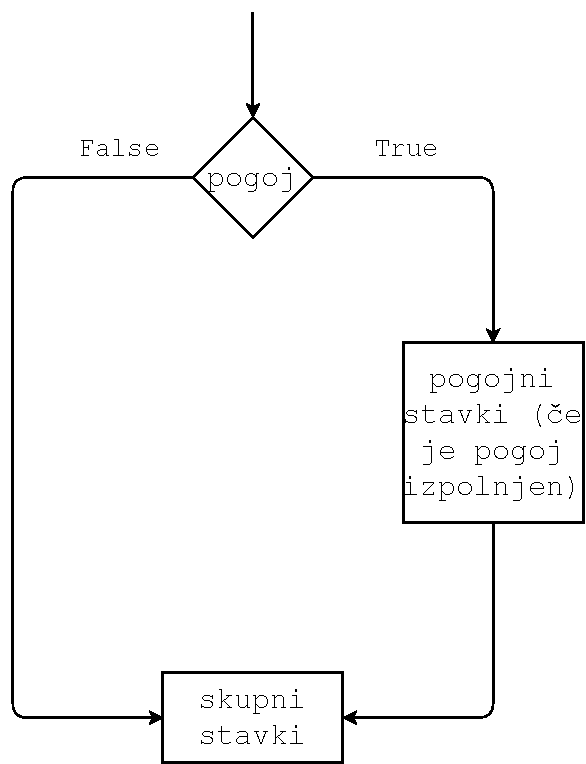
\includegraphics[width=0.5\linewidth]{img/if1.pdf}
    \caption{Diagram poteka osnovne oblike stavka \texttt{if}. V primeru, če je pogoj izpolnjen, se izvede pogojni del.}
    \label{img:if1}
\end{figure}

\section{Kaj je pogoj?}

Kaj pravzaprav predstavlja pogoj za izvedbo pogojnega dela stavka? Kot je razvido iz slike \ref{img:if1} je pogoj nekaj, kar je lahko resnično \angl{true} ali neresnično \angl{false}. Pogoj moramo torej zastaviti kot vprašanje, na katerega lahko odgovorimo bodisi z odgovorom \emph{da} ali z odgovorom \emph{ne}. Pri formiranju vprašanja oziroma pogoja bomo torej večinoma uporabljali operatorje, ki vračajo take odgovore. Tem operatorjem pravimo \emph{pogojni operatorji} pa si poglejmo nekaj njihovih primerov.

\subsection{Primerjalni operatorji in podatkovni tip \texttt{bool}}

Prva skupina operatorjev, ki jih bomo uporabljali pri pisanju pogojev so t.i. \emph{primerjalni operatorji}, ki jih poznamo že iz matematike. To so npr. operator enakosti \texttt{==} (ker je enojni enačaj uporabljen za prirejanje, moramo za primerjanje uporabiti dvojni enačaj), operator neenakosti \texttt{!=}, večji \texttt{>}, večji ali enak \texttt{>=} itd. Poskusimo:
\begin{lstlisting}[language=Python, showstringspaces=false]
>>> 1 == 1
True
>>> 1 == 2
False
>>> 1 != 2
True
>>> 1 > 2
False
>>> 1 <= 2
True
>>> 1 == 2.5
False
>>> 1 == 1.0
True
\end{lstlisting}
S primerjalnimi operatorji torej lahko primerjamo med seboj dva podatka, rezultat primerjanja pa je bodisi vrednost \texttt{True} ali \texttt{False}. Rezultat primerjanja je podatek, ki lahko zavzame samo te dve vrednosti. Kakšen je podatkovni tip tega podatka?
\begin{lstlisting}[language=Python, showstringspaces=false]
>>> type(True)
<class 'bool'>
>>> type(False)
<class 'bool'>
\end{lstlisting}
Za oblikovanje pogojev imamo torej na voljo poseben podatkovni tip, tj. \texttt{bool}, oziroma po angleško \emph{boolean}, ki lahko zavzame samo dve vrednosti, tj. \texttt{True} ali \texttt{False}. 

Poskusimo uporaba primerjalnih operatorjev uporabiti na zgledu iz začetka poglavja.
\begin{zgled}
Napiši program, ki od uporabnika prebere telesno maso in višino in izpiše uporabnikov indeks telesne mase (ITM). Poleg tega program uporabniku pove, v katero skupino spada. 
\end{zgled}
\begin{resitev}
Program od prej bomo dopolnili s pogojnim stavkom. Če je ITM manjši od 17.5, lahko program izpiše, da je uporabnikova telesna masa premajhna. Če je ITM večji od 25, lahko program izpiše, da je uporabnikova telesna masa prevelika. Kaj pa vmes? Tega pa zaenkrat še ne znamo. 
\begin{lstlisting}[language=Python, showstringspaces=false,numbers=left]
masa = float(input("Vpiši svojo telesno maso [kg]: "))
visina = float(input("Vpiši svojo višino [m]: "))
itm = masa/visina**2
print("Tvoj ITM je", itm)
if ITM < 17.5:
    print("Tvoja telesna masa je premajhna")
if ITM > 25:
    print("Tvoja telesna masa je prevelika")
\end{lstlisting}
\end{resitev}

Primerjalne operatorje lahko uporabimo tudi nad podatki, ki niso števila
\begin{lstlisting}[language=Python, showstringspaces=false]
>>> "abc" == "abc"
True
>>> "abc" == "ABC"
False
>>> "abc" < "b"
True
>>> "abc" < "abc"
False
>>> "abc" < "abd"
True
\end{lstlisting}
Iz zgornjih zgledov vidimo tudi to, da Python loči med velikimi in malimi črkami in da so določeni nizi manjši od drugih. Kako pa primerjanje dveh nizov poteka? Na enak način, kot primerjamo nize, ko poskušamo besede sortirati po abecedi (npr. v slovarju ali telefonskem imeniku). Dve besedi primerjamo znak po znaku od začetka do konca, dokler ne pridemo do dveh znakov, ki se razlikujeta ali do konca ene izmed besed. Če se besedi ujemata po vseh znakih in je ena beseda krajša, je krajša beseda zagotovo manjša. Npr., beseda "Beda" je manjša od besede "Bedarija" (v slovarju bo verjetno Beda nastopala pred Bedarijo):
\begin{lstlisting}[language=Python, showstringspaces=false]
>>> "Beda" < "Bedarija"
True
\end{lstlisting}
Beseda "Bedno" pa ni manjša od besede "Bedarija", čeprav je od nje krajša. Zakaj ne? Zato, ker se besedi razlikujeta v četrtem primerjanju na znakih "n" in "a" in ker "n" pač ni manjši od znaka "a".
\begin{lstlisting}[language=Python, showstringspaces=false]
>>> "Bedno" < "Bedarija"
False
\end{lstlisting}
Takemu primerjanju pravimo \emph{leksikografsko} primerjanje. 

\subsection{Operatorja vsebovanosti}

Ko smo ravno pri nizih, lahko nad njimi definiramo še \emph{operatorja vsebovanosti}, ki preverjata ali nekaj je (\texttt{in}) oziroma ni (\texttt{not in}) v posameznem nizu vsebovano. Operatorja bomo uporabljali tudi na drugih podatkovnih tipih, ki podobno kot nizi, vsebujejo druge podatke -- nizi so sestavljeni iz več znakov oziroma podnizov. Če je nek niz \texttt{podniz} vsebovan v nekem nizu \texttt{niz}, lahko preverim takole:
\begin{lstlisting}[language=Python, showstringspaces=false]
>>> podniz in niz
\end{lstlisting}
Povadimo:
\begin{lstlisting}[language=Python, showstringspaces=false]
>>> "Beda" in "Bedarija"
True
>>> "beda" in "Bedarija"
False
>>> "ana" in "anakonda"
True
>>> "a" in "abeceda"
True
\end{lstlisting}
Spet vidimo, da je znak \texttt{"b"} nekaj drugega kot znak \texttt{"B"} in da Python loči med malimi in velikimi črkami.

\subsection{Združevanje rezultatov primerjanja}

Pri reševanju naloge z izpisovanjem podatkov o ITM imamo še vedno težave s primerom, kjer morata biti izpolnjena dva pogoja hkrati (\texttt{ITM >= 18.5} in \texttt{ITM <= 25}). Končen pogoj za izvedbo izpisa \texttt{Tvoja telesna masa je ustrezna}, moramo torej sestaviti iz dveh pogojev. Za ta namen lahko uporabimo t.i. \emph{logične operatorje}, ki omogočajo medsebojno združevanje več spremenljivk tipa \texttt{bool}. Osnovna logična operatorja, ki ju bomo uporabljali v takem primeru sta operator \texttt{and} in operator \texttt{or}. Njuno delovanje lahko ponazorimo s spodnjo tabelo:

\begin{tabular}{cc|cc}
     \texttt{pogoj1} & \texttt{pogoj2}  & \texttt{pogoj1 and pogoj2} & \texttt{pogoj1 or pogoj2}\\
     \hline
     \texttt{False} & \texttt{False} & \texttt{False} & \texttt{False} \\
     \texttt{False} & \texttt{True} & \texttt{False} & \texttt{True} \\
     \texttt{True} & \texttt{False} & \texttt{False} & \texttt{True} \\
     \texttt{True} & \texttt{True} & \texttt{True} & \texttt{True} \\
\end{tabular}

V primeru, da morata biti izpolnjena oba vhodna pogoja, torej uporabimo operator \texttt{and}. Če je dovolj, da je izpolnjen samo eden izmed vhodnih pogojev, uporabimo operator \texttt{or}. Pogosto uporabljen logični operator je še operator \texttt{not}, ki \texttt{True} spremeni v \texttt{False} in obratno:
\begin{lstlisting}[language=Python, showstringspaces=false]
>>> not True
False
>>> not False
True
\end{lstlisting}

Zdaj lahko dokončamo zgled z izpisovanjem podatkov o ITM.
\begin{zgled}
Napiši program, ki od uporabnika prebere telesno maso in višino in izpiše uporabnikov indeks telesne mase (ITM). Poleg tega program uporabniku pove, v katero skupino spada. 
\end{zgled}
\begin{resitev}
Zdaj lahko dodamo še pogojni stavek, pri katerem bo pogoj sestavljen iz dveh delov. V tem primeru mora biti vrednost spremenljivke \texttt{ITM} večja ali enaka od 17.5 in manjša ali enaka od 25, kar lahko zapišemo s pogojem \texttt{17.5 <= ITM and ITM <= 25}.
\begin{lstlisting}[language=Python, showstringspaces=false,numbers=left]
masa = float(input("Vpiši svojo telesno maso [kg]: "))
visina = float(input("Vpiši svojo višino [m]: "))
itm = masa/visina**2
print("Tvoj ITM je", itm)
if ITM < 17.5:
    print("Tvoja telesna masa je premajhna")
if ITM > 25:
    print("Tvoja telesna masa je prevelika")
if 17.5 <= ITM and ITM <= 25:
    print("Tvoja telesna masa je ustrezna")
\end{lstlisting}
\end{resitev}

Programiranja se učimo v jeziku Python med drugim tudi zato, ker omogoča kar nekaj uporabnih sladkorčkov (funkcionalnosti), ki jih drugi jeziki ne podpirajo. Sestavljen pogoj \texttt{17.5 <= ITM and ITM <= 25} lahko v tem jeziku zapišemo tudi malo krajše, in sicer takole: \texttt{17.5 <= ITM <= 25}.

\section{Veja \texttt{else}}

Zgornji program je sicer pravilen, ni pa najlepši. V primeru, da je npr. izpolnjen prvi pogoj, tj. \texttt{ITM < 17.5}, ni nobene potrebe po tem, da preverjamo še izpolnjenost drugega in tretjega pogoja. To sicer v tem primeru ni narobe (lahko bi bilo), je pa nepotrebno in po eni strani naredi našo kodo manj pregledno, po drugi strani pa trati dragocen procesorski čas, saj preverja, če je določen pogoj izpolnjen, kljub temu, da vemo, da zagotovo ne more biti. Potek programa, ki smo ga napisali zgoraj, ponazarja slika \ref{img:if21}.

\begin{figure}
    \centering
    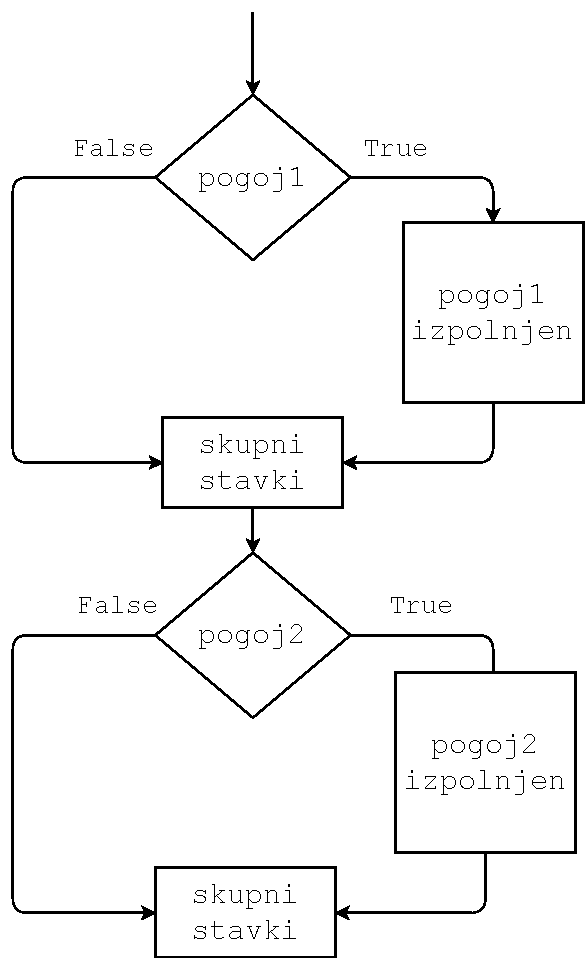
\includegraphics[width=0.5\linewidth]{img/if21.pdf}
    \caption{Izpolnjenost pogoja \texttt{pogoj2} se preverja ne glede na izpolnjenost pogoja \texttt{pogoj1}.}
    \label{img:if21}
\end{figure}

Do sedaj smo v primeru neizpolnjenosti pogoja vedno skočili na del \texttt{skupni stavki}, torej na del, ki se izvede neodvisno od izpolnjenost pogoja. V splošnem pa stavek \texttt{if} omogoča, da del kode izvedemo samo takrat, ko pogoj \textbf{ni} izpolnjen. To kodo podamo v veji \texttt{else} stavka \texttt{if}:
\begin{lstlisting}[language=Python, showstringspaces=false]
if pogoj:
    # pogojni stavki
    # če je pogoj izpolnjen
    ...
else:
    # pogojni stavki
    # če pogoj ni izpolnjen
    ...
# skupni stavki
...
\end{lstlisting}
Potek izvajanja zgornje kode prikazuje slika \ref{img:if2}. 

\begin{figure}
    \centering
    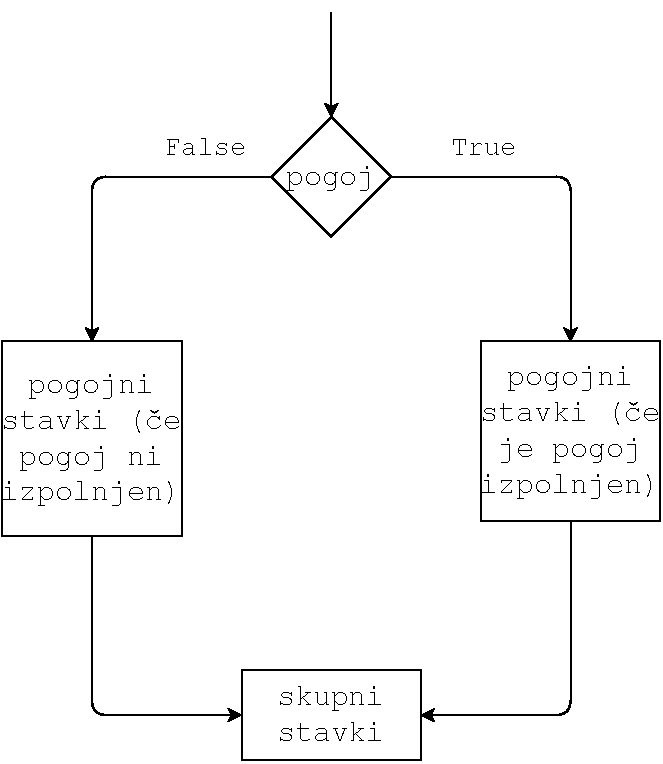
\includegraphics[width=0.5\linewidth]{img/if2.pdf}
    \caption{Dopolnitev stavka \texttt{if} z vejo \texttt{else}. Veja \texttt{else} se izvede samo v primeru, ko pogoj ni izpolnjen.}
    \label{img:if2}
\end{figure}

Uporabimo zgornji stavek za poenostavljeno rešitev naloge z izpisovanjem podatkov o ITM.
\begin{zgled}
Napiši program, ki od uporabnika prebere telesno maso in višino in izpiše uporabnikov indeks telesne mase (ITM). Poleg tega program uporabniku pove, če je njegova telesna masa ustrezna ali ne. 
\end{zgled}
\begin{resitev}
Tokrat bomo preverjali le pogoj o ustreznosti uporabnikove teže. 
\begin{lstlisting}[language=Python, showstringspaces=false,numbers=left]
masa = float(input("Vpiši svojo telesno maso [kg]: "))
visina = float(input("Vpiši svojo višino [m]: "))
itm = masa/visina**2
print("Tvoj ITM je", itm)
if 17.5 <= ITM and ITM <= 25:
    print("Tvoja telesna masa je ustrezna")
else:
    print("Tvoja telesna masa ni ustrezna")
\end{lstlisting}
\end{resitev}

\section{Veja \texttt{elif} in gnezdenje stavkov \texttt{if}}

Uporabnik zdaj ve, če je njegova telesna masa ustrezna. Če njegova telesna masa ni ustrezna, informacije o tem ali je pretežak ali prelahek nima (verjetno se mu to sicer dozdeva). Zgornji primer bi torej radi dopolnili tako, da znotraj veje \texttt{else} izvedemo dodatno primerjanje, na podlagi katerega bomo lahko ugotovili ali je ITM prevelik ali premajhen.

To lahko naredimo na dva načina. Elegantnejši način je uporaba stavka \texttt{elif}, ki omogoča preverjanje dodatnega pogoja znotraj veje \texttt{else}. Celoten stavek \texttt{if} z vejo \texttt{elif} zapišemo takole:
\begin{lstlisting}[language=Python, showstringspaces=false]
if pogoj1:
    # pogojni stavki
    # pogoj1 izpolnjen
    ...
elif pogoj2:
    # pogojni stavki
    # pogoj1 ni izpolnjen
    # pogoj2 izpolnjen
    ...
else:
    # nobeden izmed pogojev
    # ni izpolnjen
# skupni stavki
...
\end{lstlisting}
V tem primeru se izpolnjenost pogoja \texttt{pogoj2} preverja samo, če pogoj \texttt{pogoj1} ni izpolnjen, veja \texttt{else} pa se izvede samo v primeru, ko ni bil izpolnjen nobeden izmed prejšnjih pogojev. Potek programa prikazuje slika \ref{img:if3}.

\begin{figure}
    \centering
    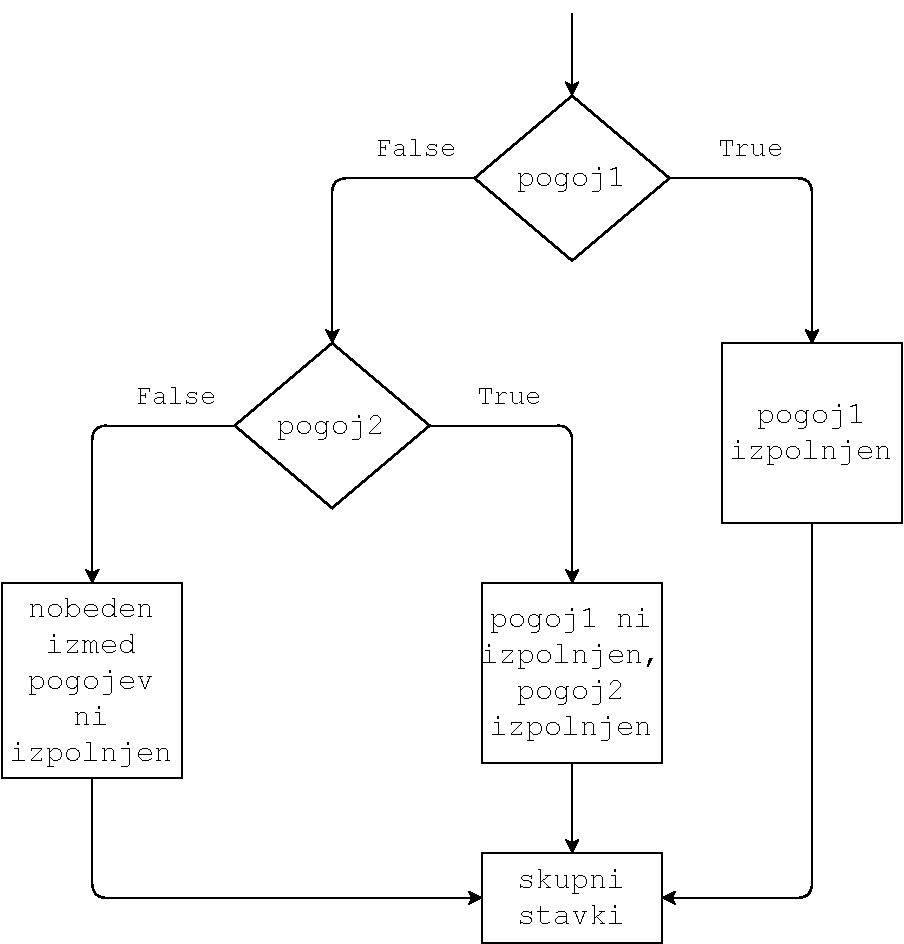
\includegraphics[width=0.65\linewidth]{img/if3.pdf}
    \caption{Dopolnitev stavka \texttt{if} z vejama \texttt{elif} in \texttt{else}. Veja \texttt{elif} se izvede samo v primeru, ko pogoj \texttt{pogoj1} ni izpolnjen, pogoj \texttt{pogoj2} pa je.}
    \label{img:if3}
\end{figure}

Zdaj lahko končno podamo lepšo rešitev zgleda z izpisovanjem podatkov o ITM.
\begin{zgled}
Napiši program, ki od uporabnika prebere telesno maso in višino in izpiše uporabnikov indeks telesne mase (ITM). Poleg tega program uporabniku pove, v katero skupino spada. 
\end{zgled}
\begin{resitev}
Najprej bomo preverili enega izmed pogojev, npr. če je ITM manjši od 17.5. V primeru, da je izpolnjen, izpišemo, da je telesna masa premajhna. V veji \texttt{elif} lahko preverimo naslednji pogoj, npr. če je ITM večji od 25. V primeru, da je izpolnjen, izpišemo, da je telesna masa prevelika. Če ni izpolnjen nobeden izmed obeh pogojev, lahko izpišemo, da je telesna masa ustrezna.
\begin{lstlisting}[language=Python, showstringspaces=false,numbers=left]
masa = float(input("Vpiši svojo telesna masa [kg]: "))
visina = float(input("Vpiši svojo višino [m]: "))
itm = masa/visina**2
print("Tvoj ITM je", itm)
if ITM < 17.5:
    print("Tvoja telesna masa je premajhna")
elif ITM > 25:
    print("Tvoja telesna masa je prevelika")
else:
    print("Tvoja telesna masa je ustrezna")
\end{lstlisting}
\end{resitev}

Drug pristop k reševanju enakega problema je uporaba dodatnega stavka \texttt{if} znotraj veje \texttt{else}. Temu rečemo tudi \emph{gnezdenje} ali \emph{ugnezdeni stavek} \texttt{if}. Kodo bi napisali takole: \begin{lstlisting}[language=Python, showstringspaces=false]
if pogoj1:
    # pogojni stavki
    # pogoj1 izpolnjen
    ...
else
    if pogoj2:
        # tukaj so uporabljeni dvojni zamiki
        # pogojni stavki
        # pogoj1 ni izpolnjen
        # pogoj2 izpolnjen
        ...
    else:
        # tukaj so uporabljeni dvojni zamiki
        # nobeden izmed pogojev
        # ni izpolnjen
# skupni stavki
...
\end{lstlisting}
Začetek ugnezdenega stavka \texttt{if} je zamaknjen enkrat, s čimer povemo, da naj se izvede samo v primeru, ko pogoj \texttt{pogoj1} ni izpolnjen. Vsebino ugnezdenega stavka moramo zamakniti dvakrat. Izvedba zgornje kode bo enaka kot v primeru z uporabo veje \texttt{elif} in jo prikazuje slika \ref{img:if3}. 

Uporabimo ugnezden stavek \texttt{if} še pri reševanju naše naloge.
\begin{zgled}
Napiši program, ki od uporabnika prebere telesno maso in višino in izpiše uporabnikov indeks telesne mase (ITM). Poleg tega program uporabniku pove, v katero skupino spada. Uporabi ugnezden stavek \texttt{if}
\end{zgled}
\begin{resitev}
Potek programa bo podoben kot prej za razliko od gnezdenje stavka \texttt{if}.
\begin{lstlisting}[language=Python, showstringspaces=false,numbers=left]
masa = float(input("Vpiši svojo telesno maso [kg]: "))
visina = float(input("Vpiši svojo višino [m]: "))
itm = masa/visina**2
print("Tvoj ITM je", itm)
if ITM < 17.5:
    print("Tvoja telesna masa je premajhna")
else
    if ITM > 25:
        print("Tvoja telesna masa je prevelika")
    else:
        print("Tvoja telesna masa je ustrezna")
\end{lstlisting}
\end{resitev}

\chapter{Zanka \texttt{while}}

\section{Kaj so zanke?}

Z uporabo stavka \texttt{if} lahko torej izbrane stavke izvedemo samo v primeru, ko je nek pogoj izpolnjen. Včasih pa bi želeli izbrane stavke izvajati vse \textbf{dokler} \angl{while} je nek pogoj izpolnjen. To omogočajo \textbf{zanke}. V sledečem poglavju si bomo podrobneje pogledali zanko \texttt{while}. 

\section{Zanka \texttt{while}}

Razliko med izvedbo pogojnega stavka \texttt{if} in zanko \texttt{while} prikazuje slika \ref{img:while_vs_if}.

\begin{figure}
    \centering
    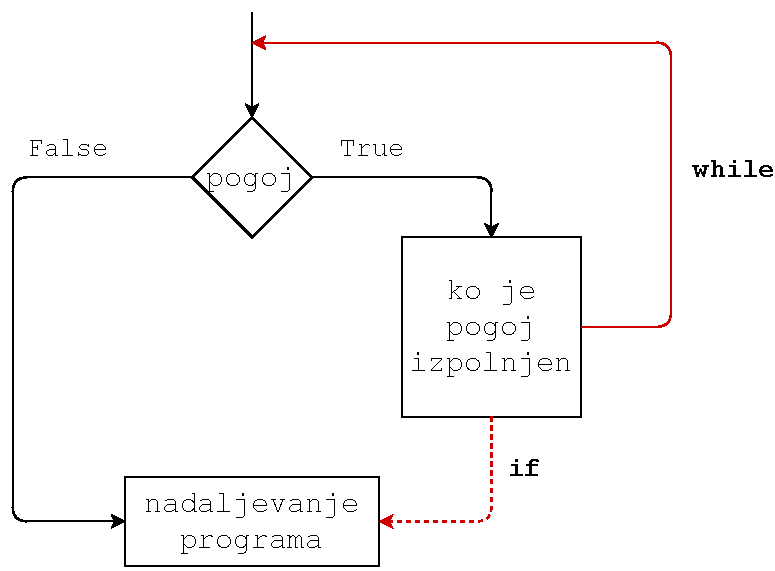
\includegraphics[width=0.5\linewidth]{img/while_vs_if.pdf}
    \caption{Razlika med izvedbo pogojnega stavka \texttt{if} (črtkana linija rdeče barve) in zanko \texttt{while} (polna linija rdeče barve). }
    \label{img:while_vs_if}
\end{figure}
Po izvedbi pogojnega dela stavka \texttt{if} se izvajanje programa nadaljuje v delu, ki sledi pogojnim stavkom. Po drugi strani se po izvedbi pogojnega dela zanke \texttt{while}, recimo tem stavkom raje \emph{telo zanke}, izpolnjenost pogoja v \emph{glavi zanke} ponovno preveri. Telo (vsebina) zanke se bo torej izvajalo vse dokler bo pogoj izpolnjen. Zanko \texttt{while} lahko zapišemo takole:
\begin{lstlisting}[language=Python, showstringspaces=false]
while pogoj: # glava zanke
    # telo zanke
    ...
# nadaljevanje programa
...
\end{lstlisting}
Zapis zanke \texttt{while} je torej zelo podoben zapisu stavka \texttt{if}. Glavi zanke sledi telo zanke oziroma njena vsebina, ki se izvaja vse dokler je pogoj izpolnjen. Enemu obhodu zanke pravimo tudi \texttt{iteracija} zanke. Pogoje za izvedbo nove iteracije zanke lahko zapisujemo na popolnoma enak način kot pri stavku \texttt{if}. Prav tako kot pri stavku \texttt{if} vsebino zanke definiramo tako, da stavke znotraj telesa zanke zamikamo. Izvajanje zanke \texttt{while} ponazarja diagram poteka na sliki \ref{img:while1}.

\begin{figure}
    \centering
    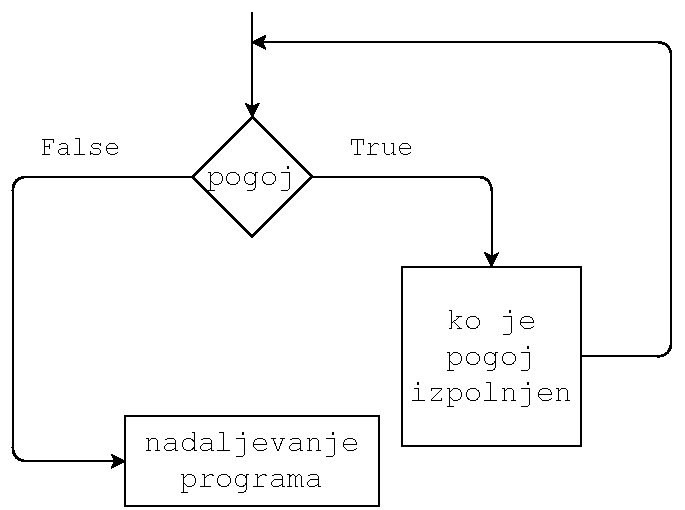
\includegraphics[width=0.5\linewidth]{img/while1.pdf}
    \caption{Potek izvajanja zanke \texttt{while}.}
    \label{img:while1}
\end{figure}

Zanke torej lahko uporabljamo takrat, ko želimo nekaj ponavljati, dokler je določen pogoj izpolnjen. Npr., dokler uporabnik ne poda veljavnega vnosa, dokler ni števec dosegel določene vrednosti ali pa dokler sta števili različni. Končno lahko rešimo program, ki išče največji skupni delitelj dveh števil.
\begin{zgled}
Napiši program, ki od uporabnika prebere dve celi števili in poišče največji skupni delitelj teh dveh števil z uporabo Evklidovega algoritma.
\end{zgled}
\begin{resitev}
Program bo manjše število odšteval od večjega, dokler sta števili različni. Uporabili bomo torej zanko \texttt{while} (dokler sta števili različni).  Znotraj zanke bomo uporabili še stavek \texttt{if}, s pomočjo katerega bomo ugotovili, katero število je manjše. 
\begin{lstlisting}[language=Python, showstringspaces=false,numbers=left]
st1 = int(input("Vnesi prvo število: "))
st2 = int(input("Vnesi drugo število: "))

while st1 != st2: # dokler sta števili različni
    if st1 < st2: # drugo število je večje
        st2 = st2 - st1
    else: # prvo število je večje
        st1 = st1 - st2

# konec vsebine zanke 
print(st1) # števili sta tu enaki, zato je vseeno katero izpišem
\end{lstlisting}
Opomba: vsebina stavka \texttt{if} je zamaknjena dvakrat, saj je zapisana tako znotraj stavka \texttt{if} kot tudi znotraj zanke \texttt{while}!
\end{resitev}

\section{Štetje z zanko \texttt{while}}

Zanko \texttt{while} bi lahko uporabili tudi za štetje. Za ta namen je sicer boljša zanka \texttt{for}, ki jo bomo spoznali malo kasneje. Poglejmo si zgled.
\begin{zgled}
Napiši program, ki šteje od 0 do števila, ki ga je vnesel uporabnik. Vsa števila naj program tudi izpiše
\end{zgled}
\begin{resitev}
Število, do katerega smo prešteli, si bomo morali nekam zabeležiti, npr. v spremenljivko z imenom \texttt{i}. Šteti bomo glede na navodila začeli s številom 0. Torej bomo spremenljivko \texttt{i} na začetku postavili na 0. Končali bomo s številom, ki ga je vnesel uporabnik, recimo \texttt{n}. Pogoj za štetje naprej bo torej \texttt{i <= n}. Znotraj zanke \texttt{while} bomo trenutno število (\texttt{i}) izpisali, poleg tega moramo trenutno število tudi povečati, saj bo sicer pogoj za vedno izpolnjen. 
\begin{lstlisting}[language=Python, showstringspaces=false,numbers=left]
n = int(input("Vpiši število do katerega želiš šteti: "))
i = 0 # števec s katerim bomo šteli
while i <= n: # smo ze prešteli do konca?
    print(i)
    i = i + 1 # povečanje števca za 1
\end{lstlisting}
\end{resitev}

\section{Stavek \texttt{+=}}
Znotraj zanke smo števec povečali za 1 z izvedbo prireditvenega stavka
\begin{lstlisting}[language=Python, showstringspaces=false]
i = i + 1 # povečanje števca za 1
\end{lstlisting}
Ker je tak način povečevanja vrednosti zelo pogost, v jeziku Python obstaja bližnjica
\begin{lstlisting}[language=Python, showstringspaces=false]
i += 1 # povečanje števca za 1
\end{lstlisting}
Bistvo zgornjega stavka je, da izvedemo aritmetično operacijo seštevanja in rezultat priredimo spremenljivki, nad katero smo operacijo izvedli. Na podoben način lahko operator prirejanja \texttt{=} kombiniramo z drugimi aritmetičnimi operatorji in števili:
\begin{lstlisting}[language=Python, showstringspaces=false]
>>> x = 10
>>> x += 1 # povečaj za 1
>>> x
11
>>> x -= 2 # zmanjšaj za 2
>>> x
9
>>> x *= 5 # pomnoži s 5
>>> x
45
>>> x /= 9 # deli z 9
>>> x
5.0
>>> x **= 2 # potenciraj na 2
>>> x
25.0
\end{lstlisting}

\section{Mrtva zanka}

Kaj pa bi se zgodilo, če bi števec v prejšnjem zgledu znotraj zanke pozabili povečati? Spremenljivka \texttt{i} (oziroma števec) bi ostala na vrednosti 0 ne glede na to koliko iteracij zanke bi se izvedlo. To pomeni, da bi bil pogoj za vedno izpolnjen (\texttt{True}). Kdaj bi se taka zanka končala? Ker je pogoj vedno resničen, se taka zanka nikoli ne konča in tak program je potrebno končati na silo (v okolju Python je temu namenjena kombinacija tipk \texttt{ctrl + c}). Na take stvari moramo torej pri programiranju z zanko \texttt{while} paziti. Zanki, ki se nikoli ne konča, pravimo \emph{mrtva zanka} \angl{deadlock}.

\section{Stavek \texttt{break}}
Zanko pa lahko prekinemo tudi drugače kot z neizpolnjenostjo pogoja v glavi zanke. Uporabimo lahko namreč stavek \texttt{break}, ki prekine izvajanje zanke brez preverjanja pogoja v glavi zanke. Primer uporabe stavka \texttt{break} ponazarja spodnja koda
\begin{lstlisting}[language=Python, showstringspaces=false]
while pogoj:
    # telo zanke
    ...
    if dodaten_pogoj: 
        break # prekine izvajanje zanke
# nadaljevanje programa
...
\end{lstlisting}
Izvedbo primera prikazuje slika \ref{img:while2}. 
\begin{figure}
    \centering
    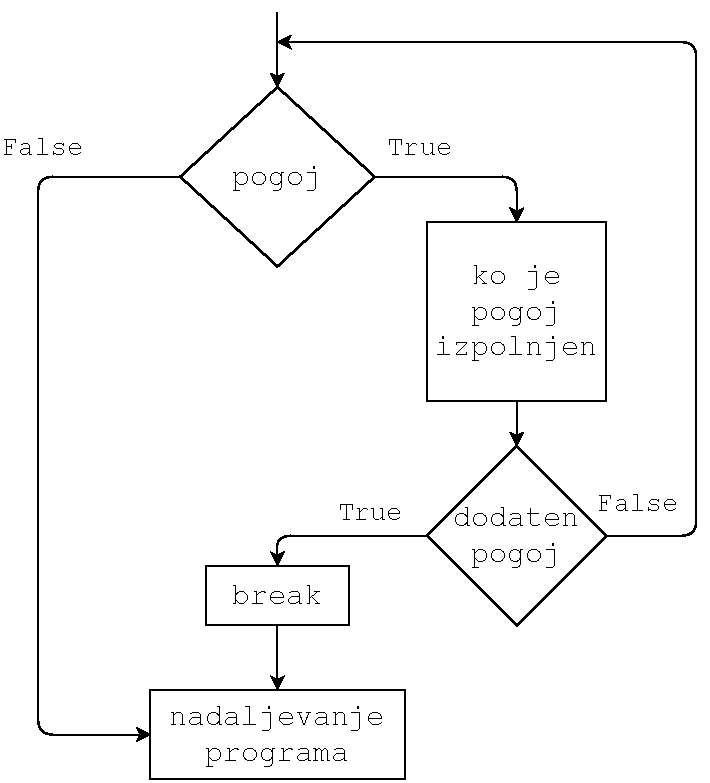
\includegraphics[width=0.5\linewidth]{img/while2.pdf}
    \caption{Primer uporabe stavka \texttt{break} znotraj zanke \texttt{while}.}
    \label{img:while2}
\end{figure}

Stavek \texttt{break} ponavadi uporabljamo v kombinaciji z dodatnim pogojem. V primeru, da je slednji izpolnjen, se izvajanje zanke prekine predčasno. Poglejmo si še en zgled, na katerem bomo potrenirali uporabo stavka \texttt{break}. 

\begin{zgled}
Napiši program, ki od uporabnika prebere dve celi števili in izpiše, če sta števili tuji. Števili sta tuji, če nimata nobenega skupnega delitelja, ki je večji od 1.
\end{zgled}
\begin{resitev}
Nalogo bi lahko rešili tako, da bi poiskali največji skupni delitelj podanih števil (naj bosta to števili \texttt{st1} in \texttt{st2}) in pogledali, če je ta večji od 1. Tokrat se bomo rešitve lotili na malo drugačen način. Preverili bomo, če med kandidati za skupne delitelje obstaja kakšno število, ki deli obe števili, pri čemer bodo kandidati v razponu od števila 2 do manjšega števila, torej do vrednosti \texttt{min(st1, st2)}. V primeru, da med kandidati najdemo eno število, ki deli obe podani števili (ostanek po deljenju posameznega števila s kandidatom je enak 0 (\texttt{st \% delitelj == 0}), lahko takoj izpišemo, da števili nista tuji.
\begin{lstlisting}[language=Python, showstringspaces=false,numbers=left]
st1 = int(input("Vnesi prvo število: "))
st2 = int(input("Vnesi drugo število: "))

delitelj = 2 # začetna vrednost kandidata

while delitelj <= min(st1, st2): # kandidat gre do manjšega
    # ali kandidat deli obe števili?
    if st1 % delitelj == 0 and st2 % delitelj == 0:
        print("Števili nista tuji")
    delitelj += 1
\end{lstlisting}
Rešitev je še nepopolna, saj izpis poda samo v primeru, ko števili nista tuji. Kako bi lahko program dopolnili, tako da bi izpis podal tudi v primeru, ko sta števili tuji. Tak izpis lahko podamo samo v primeru, ko smo pregledali vse kandidate in nismo našli nobenega, ki deli obe števili. Pomagamo si lahko s pomožno spremenljivko tipa \texttt{bool}, v katero bomo shranili informacijo o tem, ali smo že našli kašnega delitelja. Pri tem bomo na začetku predpostavljali, da delitelja ni. Če ga bomo našli, bomo predpostavko popravili. Na koncu bomo preverili, če smo kakšnega delitelja našli. Če bo odgovor ne (\texttt{nasli == False}), bomo izpisali, da sta si števili tuji.
\begin{lstlisting}[language=Python, showstringspaces=false,numbers=left]
st1 = int(input("Vnesi prvo število: "))
st2 = int(input("Vnesi drugo število: "))

delitelj = 2 # začetna vrednost kandidata
# predspostavljamo, da skupnega delitelja še nismo našli:
nasli = False 

while delitelj <= min(st1, st2): # kandidat gre do manjšega
    # ali kandidat deli obe števili?
    if st1 % delitelj == 0 and st2 % delitelj == 0:
        print("Števili nista tuji")
        nasli = True # popravimo predpostavko
    delitelj += 1

# če do tu skupnega delitelja nismo našli, potem ga ni        
if nasli == False: 
    print("Števili sta tuji")
\end{lstlisting}
Program sicer deluje pravilno, je pa njegov izpis moteč, v primeru, da najdemo več skupnih deliteljev dveh števil. Vsakič, ko najdemo skupnega delitelja, namreč izpišemo, da smo ga našli. Poleg tega bi lahko izvajanje zanke \texttt{while} prekinili takoj, ko smo našli enega skupnega delitelja, saj je to zadosten pogoj, da si števili nista tuji. Uporabimo lahko torej stavek \texttt{break}. Končna rešitev bo sledeča.
\begin{lstlisting}[language=Python, showstringspaces=false,numbers=left]
st1 = int(input("Vnesi prvo število: "))
st2 = int(input("Vnesi drugo število: "))

delitelj = 2 # začetna vrednost kandidata
# predpostavljamo, da skupnega delitelja še nismo našli:
nasli = False 

while delitelj <= min(st1, st2): # kandidat gre do manjsega
    # ali kandidat deli obe števili?
    if st1 % delitelj == 0 and st2 % delitelj == 0:
        print("Števili nista tuji")
        nasli = True # popravimo predpostavko
        break # lahko prenehamo z iskanjem
    delitelj += 1 

# če do tu skupnega delitelja nismo našli, potem ga ni        
if nasli == False: 
    print("Števili sta tuji")
\end{lstlisting}
\end{resitev}

\section{Veja \texttt{else}}
Ena izmed posebnosti jezika Python je tudi to, da lahko vejo \texttt{else} uporabljamo tudi v kombinaciji z zanko \texttt{while}. Takole:
\begin{lstlisting}[language=Python, showstringspaces=false]
while pogoj:
    # telo zanke
    ...
else:
    # ko pogoj ni več izpolnjen
    ...
# nadaljevanje programa
...
\end{lstlisting}
Veja \texttt{else} se torej izvede, ko pogoj ni več izpolnjen. Vprašanje pa je ali se veja \texttt{else} izvede vsakič, ko se izvajanje zanke zaključi? Kakšna je razlika med stavki, ki sledijo zanki \texttt{while}, in stavki znotraj veje \texttt{else} zanke \texttt{while}? 

Do bistvene razlike med vejo \texttt{else} in običajnimi stavki, ki sledijo zanki \texttt{while}, pride, kadar zanko prekinemo s stavkom \texttt{break}. V tem primeru namreč skočimo iz zanke, s čimer preskočimo tudi njeno \texttt{else} vejo. Slednja se izvede samo v primeru, ko smo zanko prekinili po \emph{običajni} poti, tj. z neizpolnjenostjo pogoja v glavi zanke.  
\begin{lstlisting}[language=Python, showstringspaces=false]
while pogoj:
    # telo zanke
    ...
    if dodaten_pogoj:
        break # prekini izvajanje zanke
else: # samo v primeru, ko zanka ni bila prekinjena z break
    # ko pogoj ni več izpolnjen
    ...
# nadaljevanje programa
...
\end{lstlisting}
Delovanje zgornjega programa ponazarja slika \ref{img:while3}.
\begin{figure}
    \centering
    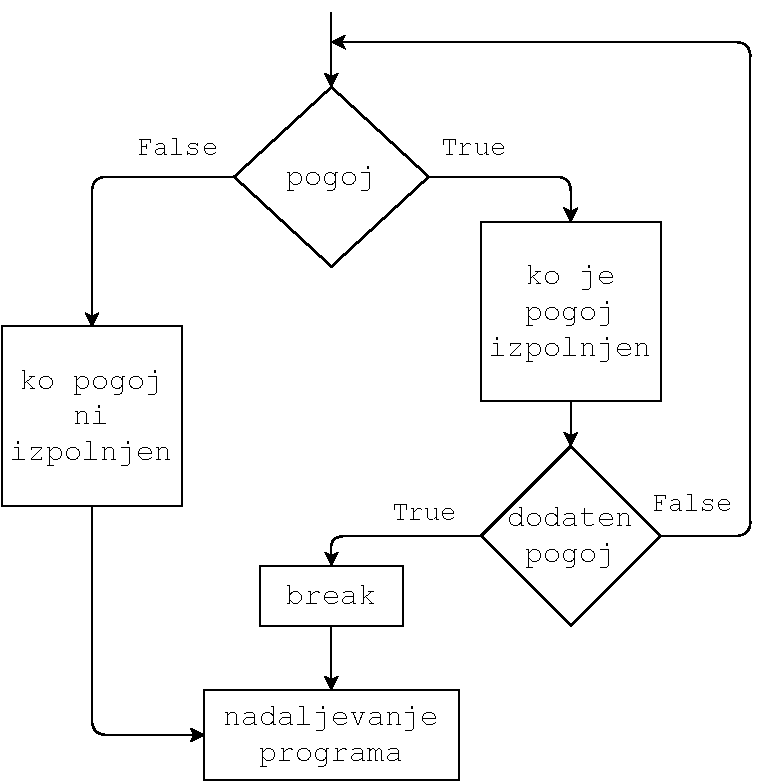
\includegraphics[width=0.5\linewidth]{img/while3.pdf}
    \caption{Primer uporabe stavka \texttt{break} v kombinaciji z vejo \texttt{else} za zanko \texttt{while}.}
    \label{img:while3}
\end{figure}
Z vejo \texttt{else} lahko določene stavke po zaključku zanke \texttt{while} izvedemo samo v primeru, ko zanka ni bila prekinjena s stavkom \texttt{break}. Povadimo na prejšnjem zgledu še tole.

\begin{zgled}
Napiši program, ki od uporabnika prebere dve celi števili in izpiše, če sta števili tuji. Števili sta tuji, če nimata nobenega skupnega delitelja, ki je večji od 1.
\end{zgled}
\begin{resitev}
Del programa, kjer izpisujemo, da si števili nista tuji, bo ostal bolj ali manj nespremenjen. Skrajšamo pa lahko tiste dela programa, ki jih potrebujemo za izpis, da sta si števili tuji. Števili sta si tuji, ko nismo našli nobenega skupnega delitelja. To se zgodi takrat, ko se je zanka \texttt{while} \emph{odvrtela} do konca in nismo našli nobenega skupnega delitelja, torej je posledično nismo prekinili s stavkom \texttt{break}. Če zanko \texttt{while} dopolnimo z vejo \texttt{else}, se bo ta izvedla natanko takrat, ko zanka ni bila prekinjena s stavkom \texttt{break}, torej takrat, ko nismo našli nobenega skupnega delitelja. Znotraj veje \texttt{else} lahko torej zapišemo, da sta si števili tuji. Na tak način se lahko znebimo spremenljivke \texttt{nasli} in naredimo program krajši in bistveno bolj pregleden.
\begin{lstlisting}[language=Python, showstringspaces=false,numbers=left]
st1 = int(input("Vnesi prvo število: "))
st2 = int(input("Vnesi drugo število: "))

delitelj = 2 # začetna vrednost kandidata

while delitelj <= min(st1, st2): # kandidat gre do manjšega
    # ali kandidat deli obe števili?
    if st1 % delitelj == 0 and st2 % delitelj == 0:
        print("Števili nista tuji")
        break # lahko prenehamo z iskanjem
    delitelj += 1 
else: # ali se je zanka odvrtela do konca
    # zanke nismo prekinili s stavkom break
    print("Števili sta tuji")
\end{lstlisting}
\end{resitev}
\chapter{Seznami in metode}

\section{Sekvenčni podatkovni tipi}

Podatkovni tipi, ki smo jih srečali do sedaj, so bili večinoma namenjeni temu, da vanje shranimo posamezen (en) podatek. V spremenljivko, ki je pripadala podatkovnemu tipu \texttt{int}, smo npr. lahko shranili eno število. V določenih primerih pa se srečamo z veliko količino med seboj podobnih podatkov, nad katerimi želimo izvajati enake ali podobne operacije. V praksi bi to lahko pomenilo, da izvajamo ponavljajoče meritve enake količine, npr. dolžine skoka smučarjev skakalcev. Kaj narediti v takem primeru? Na podlagi našega dosedanjega znanja bi lahko za vsakega skakalca definirali svojo spremenljivko, kar pa ne bi bila ravno najboljša rešitev. Prvi problem tega pristopa bi bil, da je lahko skakalcev zelo veliko. V primeru skakalcev bi bila stvar mogoče še lahko obvladljiva, kaj pa če npr. merimo prisotnost transkriptov genov v celici, ki ima par tisoč genov? Drugi problem je ta, da moramo vsako izmed spremenljivk obravnati ločeno, kar nas bo pripeljalo do ogrome količine nepregledne \emph{copy--paste} kode. Tretji problem tega pristopa je, da včasih ne vemo čisto točno koliko meritev bomo imeli in koliko spremenljivk bomo imeli (koliko bo skakalcev, koliko je genov v opazovani celici) in zato težko povemo koliko spremenljivk moramo posebej obravnati. K sreči pa obstajajo t.i. \emph{sekvenčni podatkovni tipi}, v katere lahko shranjujemo večjo količino podatkov oziroma več kot en podatek. Dodatna prednost sekvenčnih podatkovnih tipov je ta, da lahko podatke sproti dodajamo in ne potrebujemo vnaprej definirati števila podatkov, ki jih bomo na koncu imeli. Mimogrede, tudi nizi so sekvenčni podatkovni tipi, saj lahko vanje shranjujemo večjo količino podatkov, ki v tem primeru predstavljajo znake oziroma enočrkovne nize. 

\section{Kaj so seznami?}

Drug predstavnik sekvenčnih podatkovnih tipov je seznam oziroma \texttt{list}. Za razliko od nizov lahko vanj shranimo poljubne podatke, kot so npr. števila, nizi in tudi drugi seznami. Dodatna prednost uporabe seznamov je ta, da lahko elemente v seznamu dodajamo sproti, zato dolžine seznama ni treba vnaprej definirati. Lahko torej začnemo s praznim seznamom in vsakič, ko dobimo podatek o novi meritvi, tega v seznam dodamo. 

Sezname definiramo z oglatimi oklepaji \texttt{[} in \texttt{]}, znotraj katerih naštejemo elemente. Prazen seznam bi naredili takole
\begin{lstlisting}[language=Python, showstringspaces=false]
>>> prazen_seznam = []
\end{lstlisting}
Seznam, ki vsebuje približno naključne dolžine skokov smučarjev skakalcev pa takole
\begin{lstlisting}[language=Python, showstringspaces=false]
>>> dolzine = [121.4, 143.1, 105.2, 99.3]
\end{lstlisting}
V isti seznam bi lahko zapisali tudi različne podatkovne tipe, npr. 3 cela števila, 1 decimalko, 5 nizov itd., čeprav v praksi tega ne srečamo pogosto. Ponavadi v sezname shranjujejmo podatke, ki pripadajo istemu podatkovnemu tipu, saj se ti podatke nanašajo na ponavljajoče izvajanje npr. določene meritve. Na koncu lahko zato z uporabo seznamov izvedemo določene statistike, npr. kdo je skočil najdlje, kakšna je povprečna dolžina skoka, koliko ljudi je skočilo itd.

\section{Indeksiranje seznamov}
Seznami so urejeni. To pomeni, da je vrstni red, v katerem naštejemo elemente seznama, pomemben. Vsak element v seznamu ima namreč svoj \emph{indeks}. Pri tem se indeksiranje začne z najmanjšim pozitivnim številom, ki v računalništvu ni 1, ampak 0. Indeksi bodo torej šli od števila 0 do dolžine seznama -- 1. V primeru zgoraj definiranega seznama \texttt{dolzine} gredo torej indeksi od 0 do 3, saj seznam vsebuje 4 elemente:

\begin{tabular}{cccccc}
\textbf{indeksi} & & 0 & 1 & 2 & 3\\
%\hline
\texttt{dolzine} & = & \texttt{[121.4,}& \texttt{143.1,} & \texttt{105.2,} & \texttt{99.3]}
\end{tabular}

Do elementa na določenem indeksu lahko pridemo z indeksiranjem, ki ga izvedemo tako, da za imenom spremenljivke indeks zapišemo v oglatih oklepajih:
\begin{lstlisting}[language=Python, showstringspaces=false]
ime_seznama[indeks]
\end{lstlisting}
Do dolžine skoka 0-tega skakalca bi torej prišli takole:
\begin{lstlisting}[language=Python, showstringspaces=false]
>>> dolzine[0]
121.4
\end{lstlisting}

Kaj pa do zadnjega skakalca? Do dolžine seznama lahko pridemo preko vgrajene funkcije \texttt{len}:
\begin{lstlisting}[language=Python, showstringspaces=false]
>>> len(dolzine)
4
\end{lstlisting}
Funkcijo lahko torej uporabimo pri indeksiranju, kadar ne vemo točno, koliko elementov ima seznam. Do zadnjega elementa torej pridemo takole:
\begin{lstlisting}[language=Python, showstringspaces=false]
>>> dolzine[len(dolzine)-1]
99.3
\end{lstlisting}
Zakaj moramo od dolžine seznama odšteti 1? Ker smo začeli šteti s številom 0, bo zadnji indeks enak dolžini seznama -- 1. Kaj pa če vseeno poskusimo indeksirati po indeksu, ki ga v seznamu ni? V tem primeru seveda dobimo napako:
\begin{lstlisting}[language=Python, showstringspaces=false]
>>> dolzine[len(dolzine)]
Traceback (most recent call last):
  File "<pyshell#16>", line 1, in <module>
    dolzine[len(dolzine)]
IndexError: list index out of range
\end{lstlisting}
Kot smo do zdaj že večkrat videli ima Python veliko lepih lastnosti. Ena izmed njih je tudi ta, da lahko uporabljamo negativno indeksiranje, pri čemer indeks -1 predstavlja zadnji element, indeks -2 predzadnji in tako naprej. Dolžine skokov imajo torej tudi negativne indekse:

\begin{tabular}{cccccc}
\textbf{indeksi} & & -4 & -3 & -2 & -1\\
%\hline
\texttt{dolzine} & = & \texttt{[121.4,}& \texttt{143.1,} & \texttt{105.2,} & \texttt{99.3]}
\end{tabular}

Prednost takega načina indeksiranja je v tem, da lahko na zelo enostaven način pridemo do zadnjega elementa seznama (brez funkcije \texttt{len}):
\begin{lstlisting}[language=Python, showstringspaces=false]
>>> dolzine[-1]
99.3
\end{lstlisting}

Mimogrede, podobno kot lahko indeksiramo elemente seznamov, lahko indeksiramo tudi elemente nizov. Prav tako lahko dolžino niza preverimo s funkcijo \texttt{len}.
\begin{lstlisting}[language=Python, showstringspaces=false]
>>> niz = "banana"
>>> niz[0]
"b"
>>> niz[-1]
"a"
>>> len(niz)
6
\end{lstlisting}

\section{Operatorji nad seznami}

Nad seznami lahko uporabimo različne operatorje, ki smo jih do zdaj uporabljali že npr. nad nizi. Nize smo npr. lahko med seboj seštevali (temu smo sicer rekli konkatenacija oziroma lepljenje). Med seboj lahko seštevamo tudi sezname:
\begin{lstlisting}[language=Python, showstringspaces=false]
>>> [1,2,3] + [4,5,6]
[1,2,3,4,5,6]
\end{lstlisting}
Ne moremo pa seznamom prišteti nečesa, kar ni seznam, npr. števila:
\begin{lstlisting}[language=Python, showstringspaces=false]
>>> [1,2,3]+4
Traceback (most recent call last):
  File "<pyshell#20>", line 1, in <module>
    [1,2,3]+4
TypeError: can only concatenate list (not "int") to list
\end{lstlisting}
Lahko pa sezname množimo s celimi števili:
\begin{lstlisting}[language=Python, showstringspaces=false]
>>> [1,2,3]*4
[1, 2, 3, 1, 2, 3, 1, 2, 3, 1, 2, 3]
\end{lstlisting}
S čim drugim jih ni smiselno množiti, zato Python tega ne podpira:
\begin{lstlisting}[language=Python, showstringspaces=false]
>>> [1,2,3]*[4,5,6]
Traceback (most recent call last):
  File "<pyshell#22>", line 1, in <module>
    [1,2,3]*[4,5,6]
TypeError: can't multiply sequence by non-int of type 'list'
\end{lstlisting}

Nad seznami lahko uporabimo tudi operatorja vsebovanosti \texttt{in} in \texttt{not in}, ki vrneta \texttt{True} ali \texttt{False} v odvisnosti od tega ali je nekaj v seznamu vsebovano ali ne:
\begin{lstlisting}[language=Python, showstringspaces=false]
>>> 1 in [1,2,3]
True
>>> 1 not in [1,2,3]
False
\end{lstlisting}

Sezname lahko primerjamo z drugimi seznami z uporabo primerjalnih operatorjev. Takole preverjamo enakost oziroma neenakost dveh seznamov:
\begin{lstlisting}[language=Python, showstringspaces=false]
>>> [1,2,3] == [1,2,3]
True
>>> [1,2,3] != [1,2,3]
False
\end{lstlisting}
Lahko tudi ugotavljamo, če je prvi seznam manjši od drugega (besedico manjši bi lahko zamenjali tudi z večji, manjši ali enak ter večji ali enak):
\begin{lstlisting}[language=Python, showstringspaces=false]
>>> [1,2,3] < [1,2,3,4]
True
>>> [1,3,3] < [1,2,3]
False
\end{lstlisting}
Primerjalni operatorji nad seznami delujejo podobno kot nad nizi, in sicer se gre za leksikografsko primerjanje. Leksikografsko primerjanje je npr. uporabljeno pri sortiranju besed v slovarju. Deluje tako, da med seboj primerjamo istoležne elemente seznama, dokler ne pridemo do neenakosti oziroma do konca enega izmed obeh seznamov. V zgornjem primeru smo prišli do konca prvega seznama. Ker je nekaj kar ne obstaja načeloma manjše kot nekaj kar obstaja, je Python vrnil, da je prvi seznam manjši od drugega. V drugem primeru se je primerjanje ustavilo pri elementih na indeksu 1, saj sta elementa na tem indeksu različna. Ker 3 ni manjše od 2, je Python ugotovil, da prvi seznam ni manjši od drugega in vrnil rezultat \texttt{False}.

\section{Spreminjanje in brisanje elementov seznama}

Videli smo že, da lahko do elementov seznama dostopamo preko indeksiranja. Preko indeksiranja pa lahko vrednosti v seznamih tudi spreminjamo. Kako? Tako, da indeksiranje seznama dopolnimo s prireditvenim stavkom:
\begin{lstlisting}[language=Python, showstringspaces=false]
seznam[indeks] = nova_vrednost
\end{lstlisting}

Tudi brisanje elementov iz seznama lahko izvajamo s pomočjo indeksiranje, le da tokrat pred indeksiranjem uporabimo besedico \textbf{\texttt{del}}:
\begin{lstlisting}[language=Python, showstringspaces=false]
del seznam[indeks]
\end{lstlisting}

\section{Vgrajene funkcije nad seznami}
Srečali smo že funkcijo \texttt{len}, s pomočjo katere lahko ugotovimo kakšna je dolžina seznama. Nad seznami pogosto uporabljamo še druge vgrajene funkcije, izmed katerih so pogosto uporabljene \texttt{min}, \texttt{max} in \texttt{sum}.

Funkcija \texttt{min} vrne najmanjši, funkcija \texttt{max} pa največji element v seznamu glede na relacijo \texttt{<}. Zdaj lahko končno ugotovimo kakšna je bila dolžina najdaljšega skoka:
\begin{lstlisting}[language=Python, showstringspaces=false]
>>> max(dolzine)
143.1
\end{lstlisting}

Izračunamo lahko tudi povprečno dožino skoka
\begin{lstlisting}[language=Python, showstringspaces=false]
>>> sum(dolzine)/len(dolzine)
117.25
\end{lstlisting}
Nad seznami lahko uporabimo še druge vgrajene funkcije. Nekatere izmed njih bomo srečali kasneje, druge pa boste zagotovo našli, če se bo takšna potreba pokazala. 

\section{Metode}

Nad seznami lahko torej uporabljamo vgrajene funkcije, ki so pač v Pythonu na voljo. Te funkcije lahko sicer uporabimo na poljubnem podatku, ki ni nujno seznam. Obstaja poseben nabor funkcij, ki pa jih lahko uporabljamo samo nad seznami. 

Tem funkcijam pravimo \emph{metode seznamov}. V splošnem se izraz \emph{metode} uporablja za posebno družino funkcij, ki pripadajo določenemu \emph{objektu}. Kaj je objekt zaenkrat ne bomo podrobneje razlagali. Lahko pa povemo, da so seznami objekti (pravzaprav je skoraj vse v Pythonu objekt). Kakorkoli že metode so tiste funkcije, ki pripadajo določenemu objektu. Do posamezne metode seznama lahko pridemo s spodnjim klicem:
\begin{lstlisting}[language=Python, showstringspaces=false]
ime_seznama.ime_metode(argumenti)
\end{lstlisting}
Klic metode je torej podoben klicu običajne funkcije, le da moramo pred imenom metode podati ime objekta, preko katerega oziroma nad katerim metodo kličemo, imeni pa ločimo s piko (\texttt{.}).

Če delamo v okolju IDLE ali v kakšnem še pametnejšem okolju, nam bo to po izpisu imena seznama in pikice podalo nabor metod, ki jih imamo na razpolago. Ko v okolju IDLE npr. napišemo
\begin{lstlisting}[language=Python, showstringspaces=false]
>>> dolzine.
\end{lstlisting}
se po nekaj sekundah pojavijo imena metod, ki jih lahko nad seznamom uporabimo: \texttt{append}, \texttt{copy}, \texttt{clear} itd.

Metode torej razširjajo vgrajene funkcije okolja Python in so vezane na točko določen podatkovni tip. Če bi npr. enako stvar kot zgoraj poskusili z nizom, bi dobili drug seznam metod, ki jih lahko poženemo nad nizom. Metodam kot argument za razliko od vgrajenih funkcij ni potrebno podati seznama (ali pa niza) nad katerim jih želimo izvesti, saj smo seznam (ali pa niz) podali že pred piko -- že s samim klicom smo povedali nad čim želimo metodo pognati. Metode vseeno velikokrat vsebujejo določene argumente, ki pač določijo kaj in kako naj metoda nad objektom naredi. 

Prav tako kot obstaja kar veliko vgrajenih funkcij, obstaja tudi veliko metod nad seznami. Natančneje si bomo v nadaljevanju tega poglavja pogledali tiste, ki jih uporabljamo pogosteje.

\section{Dodajanje elementov}

Dodajanje elementov v seznam je pogosta operacija, zato jo lahko izvedemo na več načinov. Enega smo pravzaprav že srečali, saj lahko za dodajanje elementov v seznam uporabimo kar operator \texttt{+}, ki omogoča lepljenje seznamov. Če želimo element seznamu dodati, bomo obstoječemu seznamu prišteli seznam, ki vsebuje ta element. Takole:
\begin{lstlisting}[language=Python, showstringspaces=false]
seznam = seznam + [element]
\end{lstlisting}
oziroma malo lepše:
\begin{lstlisting}[language=Python, showstringspaces=false]
seznam += [element]
\end{lstlisting}
Tole dvoje sicer ni popolnoma enako, ampak zaenkrat recimo, da je bolje uporabiti spodnjo različico. 

Elemente lahko v sezname dodajamo tudi preko metode \texttt{append} in metode \texttt{extend}. Obe metodi bosta dodajali na koncu seznama. Razlika je v tem, da v primeru metode \texttt{append} dodajamo en element, zato ta metoda kot argument prejme element, ki ga bomo v seznam dodali. Dodajanje bi torej izvedli takole:
\begin{lstlisting}[language=Python, showstringspaces=false]
seznam.append(element)
\end{lstlisting}
Metoda sicer ne bo ničesar vrnila, bo pa naš seznam spremenila. Primer uporabe je sledeč:
\begin{lstlisting}[language=Python, showstringspaces=false]
>>> seznam = [1,2,3]
>>> seznam.append(4)
>>> seznam
[1,2,3,4]
\end{lstlisting}
Podobno lahko uporabimo metodo \texttt{extend}, ki v seznam dodaja drug seznam. Kot argument moramo torej metodi \texttt{extend} podati seznam, ki ga želimo v obstoječ seznam dodati. Takole:
\begin{lstlisting}[language=Python, showstringspaces=false]
seznam.extend(seznam2)
\end{lstlisting}
Oziroma na prejšnjem zgledu takole:
\begin{lstlisting}[language=Python, showstringspaces=false]
>>> seznam = [1,2,3]
>>> seznam.extend([4])
>>> seznam
[1,2,3,4]
\end{lstlisting}

Povadimo dodajanje elementov v seznam na praktičnem zgledu.
\begin{zgled}
Napiši program, ki ga bo lahko uporabil sodnik smučarskih skokov. Program naj sodnika sprašuje po dolžini skoka. V primeru, da sodnik vnese število večje od 0, naj program to število doda v seznam in sodnika vpraša po novi dolžini. Če sodnik vpiše številko 0, naj program izpiše dolžino najdaljšega skoka in povprečno dolžino skoka.
\end{zgled}
\begin{resitev}
Sodnikova števila lahko beremo preko funkcije \texttt{input}, katere rezultat moramo pretvoriti v podatkovni tip \texttt{float}, saj so dolžine decimalna števila. Beremo dokler sodnik ne vnese števila 0, medtem pa dolžine dodajamo v seznam. Na koncu izračunamo povprečno dolžino skoka, poleg tega pa izpišemo tudi najdaljši skok. Program je sledeč:
\begin{lstlisting}[language=Python, showstringspaces=false,numbers=left]
dolzine = [] # na zacetku ni nobene dolzine
d = float(input("Vpisi dolzino: ")) # prvo branje
while d > 0: # dokler je dolzina veljavna
    dolzine.append(d) # dodaj dolzino
    d = float(input("Vpisi dolzino: ")) # ponovno branje
print("Najdaljsi skok:", max(dolzine))
print("Povprecna dolzina:", sum(dolzine)/len(dolzine))
\end{lstlisting}
\end{resitev}
Prednost zgornjega programa je v tem, da deluje ne glede na to koliko skokov je v seznamu. Vse dokler sodnik ne vnese kakšne neumnosti.

\section{Branje seznamov iz ukazne vrstice}
Včasih pa bi si želeli celoten seznam prebrati z enim samim uporabnikovim vnosom. Torej bomo spet uporabili funkcijo \texttt{input}. Spomnimo se, da funkcija \texttt{input} uporabnikov vnos vedno zapiše v niz oziroma v podatkovni tip \texttt{str}, ne glede na to kaj je uporabnik vnesel. Tak niz smo v prejšnjih primerih s funkcijo \texttt{int} pretvorili v celo število ali pa s funkcijo \texttt{float} v decimalno, če smo želeli podan vnos v nadaljevanju obravnavati kot število. Kaj pa če bi želeli niz, ki ga je vnesel uporabnik, pretvoriti v seznam? Na prvo žogo bi lahko rekli, da pač uporabimo funkcijo \texttt{list}. Poskusimo:
\begin{lstlisting}[language=Python, showstringspaces=false]
>>> seznam = list(input("Vnesi seznam: "))
Vnesi seznam: [1,2,3]
>>> seznam
['[', '1', ',', '2', ',', '3', ']']
\end{lstlisting}
To torej ni tisto, kar smo želeli. Dobili smo namreč seznam vseh znakov, ki v podanem nizu nastopajo (vključno z vejicami in oklepaji).

Kaj bi pravzaprav radi dosegli? To, da se niz, ki ga uporabnik poda funkciji \texttt{input} obravnava na enak način, kot če bi isti niz vpisal v ukazno vrstico. Temu je namenjena funkcija \texttt{eval}, ki kot argument sprejme niz in ga izvede kot Python kodo. Poskusimo še to:
\begin{lstlisting}[language=Python, showstringspaces=false]
>>> seznam = eval(input("Vnesi seznam: "))
Vnesi seznam: [1,2,3]
>>> seznam
[1,2,3]
\end{lstlisting}
V tem primeru stvar deluje, kot bi si želeli. Povadimo še na zgledu.

\begin{zgled}
Napiši program, ki ga bo lahko uporabil sodnik smučarskih skokov. Programu naj sodnik vnese seznam dolžin smučarskih skokov, program pa naj izpiše dolžino najdaljšega skoka in povprečno dolžino skoka.
\end{zgled}
\begin{resitev}
Rešitev bo podobna kot prej, le da tokrat ne potrebujemo zanke.
\begin{lstlisting}[language=Python, showstringspaces=false,numbers=left]
dolzine = eval(input("Vnesi dolzine: "))
print("Najdaljsi skok:", max(dolzine))
print("Povprecna dolzina:", sum(dolzine)/len(dolzine))
\end{lstlisting}
Slabost programa je ta, da mora sodnik zdaj vse dolžine vnesti naenkrat. 
\end{resitev}

Uporaba funkcije \texttt{eval} je sicer lahko v določenih primerih nevarna (če imamo zlobne uporabnike), saj bo slepo izvedla kodo, ki jo bo uporabnik preko vnosa podal.

\section{Sortiranje seznamov}

Zaenkrat znamo določiti najdaljši skok, ne znamo pa določiti najdaljših treh skokov. Najdaljše tri skoke bi lahko poiskali tako, da seznam uredimo (posortiramo), tako da vsebuje skoke od najdaljšega do najkrajšega. Potem izpišemo skoke na indeksih 0, 1 in 2. 

Sortiranje seznamov lahko izvedemo z metodo \texttt{sort}:
\begin{lstlisting}[language=Python, showstringspaces=false]
>>> dolzine.sort()
>>> dolzine
[99.3, 105.2, 121.4, 143.1]
\end{lstlisting}
Metoda \texttt{sort} torej sortira seznam, nad katerim smo jo poklicali, in ničesar ne vrača. Opazimo tudi, da je seznam sortirala od najmanjše vrednosti do največje. Najboljše skoke bi torej lahko izpisali tako, da bi izpisali zadnje tri dolžine iz seznama. Lahko pa seznam sortiramo v obratnem vrstnem redu, tako da metodi \texttt{sort} nastavimo opcijski (izbirni) argument \texttt{reverse} na vrednost \texttt{True}. Do dokumentacije metode \texttt{sort} lahko pridemo preko funkcije \texttt{help}:
\begin{lstlisting}[language=Python, showstringspaces=false]
>>> help(list.sort)
Help on method_descriptor:

sort(self, /, *, key=None, reverse=False)
    Stable sort *IN PLACE*.
\end{lstlisting}
Dokumentacija ni nič kaj preveč izčrpna, vidimo pa lahko, da metoda sort sprejema tudi dva opcijska argumenta, in sicer \texttt{key}, ki je privzeto enak vrednosti \texttt{None} in \texttt{reverse}, ki je privzeto enak vrednosti \texttt{False}. Opcijski argumenti so tisti argumenti, ki imajo nastavljene privzete vrednosti. Če ob klicu ne specificiramo drugačnih vrednosti, bodo pač uporabljene privzete vrednosti. Privzete vrednosti pa lahko \emph{povozimo}, tako da specificiramo drugačne vrednosti. Vrstni red urejanja bi lahko spremenili tako, da bi argument \texttt{reverse} nastavili na vrednost \texttt{True}. V našem primeru takole:
\begin{lstlisting}[language=Python, showstringspaces=false]
>>> dolzine.sort(reverse=True)
>>> dolzine
[143.1, 121.4, 105.2, 99.3]]
\end{lstlisting}

Rešimo zdaj celoten zgled od začetka do konca.
\begin{zgled}
Napiši program, ki ga bo lahko uporabil sodnik smučarskih skokov. Programu naj sodnik poda seznam dolžin smučarskih skokov, program pa naj izpiše najdaljše tri skoke.
\end{zgled}

\begin{resitev}
Zdaj bo branju seznama sledilo sortiranje in izpis zmagovalnih dolžin.
\begin{lstlisting}[language=Python, showstringspaces=false,numbers=left]
dolzine = eval(input("Vnesi dolzine: "))
dolzine.sort(reverse=True)
print("1. mesto", dolzine[0])
print("2. mesto", dolzine[1])
print("3. mesto", dolzine[2])
\end{lstlisting}
\end{resitev}

Prej smo videli, da metoda \texttt{sort} sprejema tudi izbirni argument \texttt{key}, s katerim lahko določimo, preko katerega naj funkcija sortira. Če bi želeli npr. sortirati seznam po absolutnih vrednostih, bi argumentu \texttt{key} priredili funkcijo \texttt{abs}. Takole:
\begin{lstlisting}[language=Python, showstringspaces=false]
>>> seznam = [-100, 10, -1, -5, 50]
>>> seznam.sort(key=abs)
>>> seznam
[-1, -5, 10, 50, -100]
\end{lstlisting}

Sezname (in še kaj drugega) pa bi lahko sortirali tudi preko vgrajene funkcije \texttt{sorted}. Ta funkcija deluje na enak način kot metoda \texttt{sort}, le da podanega seznama ne sortira, ampak vrne sortiran seznam. Poglejmo si na zgledu:
\begin{lstlisting}[language=Python, showstringspaces=false]
>>> seznam = [-100, 10, -1, -5, 50]
>>> # funkciji kot argument podamo tisto kar zelimo posortirati
>>> sorted(seznam) 
[-1, -5, 10, 50, -100]
>>> seznam # podan seznam je ostal nespremenjen
[-100, 10, -1, -5, 50]
\end{lstlisting}
Funkcija torej vrne sortiran seznam, izhodiščni seznam pa je ostal nespremenjen. Kako bi dosegli, da se ime spremenljivke, preko katerega smo funkcijo poklicali, spremeni, tako da vsebuje sortiran seznam? Tako, da bi rezultat funkcije \texttt{sorted} priredili spremenljivki:
\begin{lstlisting}[language=Python, showstringspaces=false]
>>> seznam = [-100, 10, -1, -5, 50]
>>> seznam = sorted(seznam)
>>> seznam
[-1, -5, 10, 50, -100]
\end{lstlisting}

\section{Seznami seznamov}

Vemo že veliko več kot prej, še vedno pa ne vemo kdo je skočil največ in komu moramo podeliti medalje. Poleg dolžin bi si namreč v ta namen morali beležiti tudi imena tekmovalcev skakalcev. To lahko rešimo tako, da imamo pač dva seznama, tj. seznam dolžin in seznam tekmovalcev. Na istoležnem indeksu imamo v obeh seznamih podatke o istem skakalcu. Takole:
\begin{lstlisting}[language=Python, showstringspaces=false]
>>> dolzine = [121.4, 143.1, 105.2, 99.3]
>>> skakalci = ["Andrej", "Bojan", "Cene", "Dejan"]
\end{lstlisting}
Andrej je torej skočil 121.4 metra, Dejan pa zgolj 99.3 metra. Zmagovalne tri skoke še vedno lahko dobimo tako, da sortiramo seznam dolžin:
\begin{lstlisting}[language=Python, showstringspaces=false]
>>> dolzine.sort(reverse=True)
>>> dolzine
[143.1, 121.4, 105.2, 99.3]
\end{lstlisting}
Do problema pa pride, ker zdaj ne vemo več kateremu imenu pripada posamezna dolžina, saj smo indekse v seznamu dolžin s sortiranjem premešali. Kaj lahko naredimo? 

Alternativen pristop bi bil, da za beleženje podatkov o dolžinah in imenih uporabimo nov, vgnezden seznam. Torej naredimo seznam seznamov. Takole:
\begin{lstlisting}[language=Python, showstringspaces=false]
>>> skoki = [[121.4, "Andrej"], 
            [143.1, "Bojan"], 
            [105.2, "Cene"], 
            [99.3, "Dejan"]]
\end{lstlisting}
Kasneje bomo za take primere sicer uporabljali malo drugačno strukturo, ampak zaenkrat te še ne poznamo. Naredili smo torej seznam seznamov. Kaj se nahaja v tem primeru na indeksu 0?
\begin{lstlisting}[language=Python, showstringspaces=false]
>>> skoki[0]
[121.4, "Andrej"]
\end{lstlisting}
Seznam, ki vsebuje podatke o ničtem skakalcu. Kako pa bi prišlo do njegovega imena? Z uporabo verižnega indeksiranja oziroma tako, da po indeksiranju zunanjega seznama pač še enkrat indeksiramo notranji seznam:
\begin{lstlisting}[language=Python, showstringspaces=false]
>>> skoki[0][1]
"Andrej"
\end{lstlisting}
Kaj se bo zgodilo, če tak seznam sortiramo? Nad vgnezdenimi seznami bo za sortiranje uporabljena relacija \texttt{<}, ki smo jo v tem poglavju v povezavi s primerjanjem seznamov že srečali. Rekli smo, da relacija manjše sezname med seboj primerja leksikografsko. Najprej primerja ničti element prvega seznam z ničtim drugega. Če sta enaka, primerja prvi element prvega seznama s prvim elementom drugega seznama in tako naprej. Če bomo torej v vgnezdene sezname na ničto mesto dali dolžine na prvo mesto pa imena, bo sortiranje izvedeno po dolžinah. Po imenih bo sortiranje potekalo samo v primeru, če bosta dolžini pri dveh podseznamih enaki. Poskusimo:
\begin{lstlisting}[language=Python, showstringspaces=false]
>>> skoki.sort(reverse=True)
>>> skoki
[[143.1, 'Bojan'], [121.4, 'Andrej'], [105.2, 'Cene'],
[99.3, 'Dejan']]
\end{lstlisting}
Ker smo zdaj sortirali dolžine skokov skupaj z imeni tekmovalcev, informacije o tem kdo je skočil koliko nismo izgubili in lahko izpišemo zmagovalce, ki se nahajajo v prvih treh podseznamih na indeksu 1:
\begin{lstlisting}[language=Python, showstringspaces=false]
>>> skoki[0,1]
'Bojan'
>>> skoki[1,1]
'Andrej'
>>> skoki[2,1]
'Cene'
\end{lstlisting}
To so zmagovalci. Zapišimo celoten zgled.
\begin{zgled}
Napiši program, ki ga bo lahko uporabil sodnik smučarskih skokov. Program naj sodnika sprašuje po dolžini skoka in imenu tekmovalca. V primeru, da sodnik za dolžino vnese število večje od 0, naj program dolžino in ime doda v seznam. Če sodnik vpiše številko 0, naj program izpiše zmagovalce in dolžine njihovih skokov.
\end{zgled}
\begin{resitev}
Ponovno bomo brali dolžino po dolžino, le da bomo tokrat v primeru, da bo vnesena dolžina večja kot 0, prebrali še ime tekmovalca. Potem bomo oboje dodali v seznam skokov. Pomembno je, da na ničto mesto v podseznam shranimo dolžino skoka, saj želimo podsezname sortirati po dolžini skokov. Na koncu skoke sortiramo in izpišemo zmagovalce in dolžine zmagovalnih skokov.
\begin{lstlisting}[language=Python, showstringspaces=false,numbers=left]
skoki = [] # na zacetku ni nobenega skoka
d = float(input("Vpisi dolzino: ")) # prvo branje
while d > 0: # dokler je dolzina veljavna
    ime = input("Vpisi ime tekmovalca: ") # branje imena
    skoki.append([d,ime]) # dodajanje podseznama
    d = float(input("Vpisi dolzino: ")) # ponovno branje
skoki.sort(reverse=True)
print("1. mesto:", skoki[0][1], ", dolzina skoka:", skoki[0][0])
print("2. mesto:", skoki[1][1], ", dolzina skoka:",  skoki[1][0])
print("3. mesto:", skoki[2][1], ", dolzina skoka:", skoki[2][0])
\end{lstlisting}
\end{resitev}

\section{Generiranje seznamov s funkcijo \texttt{range}}

Do zdaj smo sezname generirali oziroma dopolnjevali na podlagi vrednosti, ki jih je podal uporabnik. Taki seznami so lahko vsebovali poljubne elemente -- pač tisto, kar je uporabnik vnesel.

V določenih primerih želimo imeti sezname s števili v podanem razponu. Praktično uporabo takih seznamov bomo podrobneje spoznali v naslednjem poglavju, zaenkrat pa si poglejmo, kako jih lahko generiramo.

Generiranje seznamov v podanem razponu omogoča vgrajena funkcija \texttt{range}. Funkcijo \texttt{range} lahko uporabljamo na tri različne načine, in sicer preko podajanja sledečih argumentov:
\begin{itemize}
\item \texttt{start}: določa začetek seznama (celo število),
\item \texttt{stop}: določa konec seznama (celo število),
\item \texttt{step}: določa korak (celo število).
\end{itemize}

Pri prvem načinu uporabe funkciji \texttt{range} podamo zgolj argument \texttt{stop}. V tem primeru bomo dobili seznam vrednosti do argumenta \texttt{stop}--1 s korakom 1. Poskusimo:
\begin{lstlisting}[language=Python, showstringspaces=false]
>>> razpon = range(10)
>>> razpon
range(0, 10)
\end{lstlisting}
Tale izpis je malo čuden. Poklicali smo funkcijo \texttt{range} in dobili \texttt{range}. Poglejmo si kakšen je podatkovni tip rezultata:
\begin{lstlisting}[language=Python, showstringspaces=false]
>>> type(razpon)
<class 'range'>
\end{lstlisting}
Rezultat funkcije \texttt{range} torej pripada \texttt{razredu} \texttt{range}, ki nam vrednosti iz razpona vrača sproti, ko jih pač potrebujemo. Zakaj tako? Funkcija \texttt{range} je varčna in ponavadi ni nobene potrebe po tem, da bi morali celoten razpon ustvariti naenkrat, ampak naenkrat potrebujemo samo en element iz razpona. S tem, ko funkcija \texttt{range} ustvari objekt, ki nam po potrebi vrne željeni element, varčuje tako s procesorjevim časom (hitrost), saj je generiranje dolgih seznamov zamudno, kot tudi s pomnlniškim prostorom, saj dolgi seznami zasedejo veliko prostora. Še vedno pa lahko nad rezultatom funkcije \texttt{range} delamo podobne stvari, kot nad seznami. Lahko jih npr. indeksiramo:
\begin{lstlisting}[language=Python, showstringspaces=false]
>>> razpon[2]
2
\end{lstlisting}
Ne moremo pa nad njimi klicati metod, ki so definirane nad običajnimi seznami:
\begin{lstlisting}[language=Python, showstringspaces=false]
>>> razpon.sort()
Traceback (most recent call last):
  File "<pyshell#98>", line 1, in <module>
    razpon.sort()
AttributeError: 'range' object has no attribute 'sort'
\end{lstlisting}
Poleg tega funkcija \texttt{print}, kot smo videli že zgoraj, ne izpiše vrednosti elementov v razponu. Če bi želeli preko funkcije \texttt{range} dobiti običajen seznam, lahko uporabimo pretvorbo v seznam preko funkcije \texttt{list}:
\begin{lstlisting}[language=Python, showstringspaces=false]
>>> razpon = range(10)
>>> seznam = list(razpon)
>>> seznam
[0, 1, 2, 3, 4, 5, 6, 7, 8, 9]
>>> type(seznam)
<class 'list'>
\end{lstlisting}
Za to pa ponavadi ni potrebe. Primerjajmo ekonomičnost funkcije \texttt{range} in generiranja običajnega seznama. To lahko poskusimo tako, da s funkcijo \texttt{range} naredimo nek relativno velik razpon števil. Npr. od 0 do $10^8$-1:
\begin{lstlisting}[language=Python, showstringspaces=false]
>>> razpon = range(10**8)
\end{lstlisting}
Tudi če imate počasen računalnik, bo generiranje razpona narejeno v trenutku. Zdaj pa poskusimo iz tega razpona narediti klasičen seznam:
\begin{lstlisting}[language=Python, showstringspaces=false]
>>> seznam = list(razpon)
\end{lstlisting}
Če vam Python ni javil napake \texttt{MemoryError}, je tole verjetno nekaj časa trajalo. Če ni in vas nisem prepričal, poskusite stvar ponoviti z večjim številom, npr. $10^{10}$. 

Vrnimo se k osnovni uporabi funkcije \texttt{range}. Mogoče se sprašujetete zakaj razpon ne vključuje vrednosti \texttt{stop}. Razlogov za to je več. Zaenkrat podajmo najbolj očitnega. Ker funkcija \texttt{range} začne šteti z vrednostjo 0 (in ne z 1), bo razpon, ki ga bo vračala, vseboval točno \texttt{stop} elementov. Če bi funkciji \texttt{range} za argument \texttt{stop} podali dolžino nekega seznama, bi razpon vseboval vse indekse tega seznama (ena izmed možnih uporab funkcije \texttt{range} se že počasi odkriva). 

S funkcijo \texttt{range} lahko generiramo razpon elementov, ki se ne začne s številom 0. V tem primeru bomo funkciji poleg argumenta \texttt{stop} podali še argument \texttt{start}. Najprej seveda navedemo \texttt{start}, potem pa \texttt{stop}:
\begin{lstlisting}[language=Python, showstringspaces=false]
>>> range(start, stop)
\end{lstlisting}
Če bi npr. želeli generirati seznam v razponu od 5 do 10, bi napisali takole
\begin{lstlisting}[language=Python, showstringspaces=false]
>>> razpon = range(5, 10)
\end{lstlisting}
Poglejmo si seznam, ki ga s takim razponom dobimo:
\begin{lstlisting}[language=Python, showstringspaces=false]
>>> list(razpon)
[5, 6, 7, 8, 9]
\end{lstlisting}
Seznam torej vsebuje argument \texttt{start}, argumenta \texttt{stop} pa ne. Podobno kot prej. Razpon od 0 do 10 (brez števila 10) bi torej lahko dobili tudi takole:
\begin{lstlisting}[language=Python, showstringspaces=false]
>>>  razpon = range(0, 10)
>>> list(razpon)
[0, 1, 2, 3, 4, 5, 6, 7, 8, 9]
\end{lstlisting}

Do zdaj je bil korak med sosednjima elementoma v razponu vedno enak. To lahko spremenimo tako, da podamo še argument \texttt{step}. V tem primeru bomo funkcijo poklicali takole:
\begin{lstlisting}[language=Python, showstringspaces=false]
>>> range(start, stop, step)
\end{lstlisting}
Argument \texttt{step} je opcijski, njegova privzeta vrednost pa je 1. Lahko ga nastavimo na kaj drugega, npr. na 2. Če bi hoteli zgenerirati seznam lihih števil v razponu od 0 do 100, bi to lahko narediili takole:
\begin{lstlisting}[language=Python, showstringspaces=false]
>>>  razpon = range(1, 101, 2)
>>> list(razpon)
[1, 3, 5, ..., 97, 99]
\end{lstlisting}
Zakaj smo argument \texttt{start} postavili na 1? Če bi začeli šteti z 0, bi dobili seznam sodih števil.
\begin{lstlisting}[language=Python, showstringspaces=false]
>>>  razpon = range(0, 101, 2)
>>> list(razpon)
[0, 2, 4, ..., 98, 100]
\end{lstlisting}
Korak lahko nastavimo tudi na negativno vrednost:
\begin{lstlisting}[language=Python, showstringspaces=false]
>>> razpon = range(0, 101, -2)
>>> list(razpon)
[]
\end{lstlisting}
Tokrat smo dobili prazen seznam. Zakaj? Negativen korak pomeni, da štejemo navzdol. Torej mora imeti argument \texttt{start} večjo vrednost kot argument \texttt{stop}:
\begin{lstlisting}[language=Python, showstringspaces=false]
>>> razpon = range(101, 0, -2)
>>> list(razpon)
[101, 99, 97,..., 3, 1]
\end{lstlisting}
Spet smo dobili seznam lihih števil. Zakaj? Zato ker smo začeli šteti z lihim številom. Poleg tega razpon zdaj vklučuje število 101, ker je argument \texttt{start} v razponu vključen. Razpon sodih števil bi dobili takole
\begin{lstlisting}[language=Python, showstringspaces=false]
>>> razpon = range(100, 0, -2)
>>> list(razpon)
[100, 98, 96,..., 4, 2]
\end{lstlisting}
Število 0 tokrat v razponu ni vključeno, ker razpon argumenta \texttt{stop} ne vključuje. 

\section{Rezine}

V določenih primerih želimo namesto indeksiranja enega samega elementa izvesti indeksiranje razpona elementov v seznamu. Dobimo torej kos oziroma \emph{rezino} \angl{slice} seznama. Razpon seznama podamo na zelo podoben način, kot smo ga uporabljali pri funkciji \texttt{range}, in sicer preko začetka (\texttt{start}) rezine, konca (\texttt{stop}) rezine in koraka \emph{rezinjenja} (\texttt{step}).

Podamo lahko samo začetek rezine: \texttt{seznam[start:]}.  V tem primeru bo rezina odrezana do konca seznama. Če bi npr. radi dobili vse elemente seznama od vkjučno petega indeksa naprej, bi napisali takole:
\begin{lstlisting}[language=Python, showstringspaces=false]
>>> seznam = list(range(10))
>>> seznam[5:]
[5, 6, 7, 8, 9]
\end{lstlisting}
Izhodiščni seznam je kot pri običajnem indeksiranju ostal nespremenjen:
\begin{lstlisting}[language=Python, showstringspaces=false]
>>> seznam
[0, 1, 2, 3, 4, 5, 6, 7, 8, 9]
\end{lstlisting}

Podamo lahko samo konec rezine: \texttt{seznam[:stop]}.  V tem primeru se bo začela na začetku seznama in zaključila na indeksu \texttt{stop -- 1}. Podobno kot pri funkciji \texttt{range} tudi pri rezinah \texttt{stop} ni vključen v razpon. Če bi npr. radi dobili vse elemente seznama od začetka do petega indeksa (pri tem peti indeks ne bo vključen), bi napisali takole:
\begin{lstlisting}[language=Python, showstringspaces=false]
>>> seznam = list(range(10))
>>> seznam[:5]
[0, 1, 2, 3, 4]
\end{lstlisting}
Z nevključenostjo indeksa \texttt{stop} smo zopet prišli do točno \texttt{stop} vrednosti, saj se štetje začne z indeksom 0. 

Pri rezinjenju lahko podajamo tudi zgolj korak: \texttt{seznam[::step]}. V tem primeru bo rezina odrezana od začetka do konca seznama, pri čemer bo uporabljen podan korak. Če bi npr. hoteli dobiti vsak drugi element seznama, bi napisali takole:
\begin{lstlisting}[language=Python, showstringspaces=false]
>>> seznam = list(range(10))
>>> seznam[::2]
[0, 2, 4, 6, 8]
\end{lstlisting}
Korak je lahko tudi negativen. Če bi kot korak npr. napisali vrednost --1, bi s tem seznam obrnili. S tem smo namreč povedali, da gremo čez cel seznam s korakom --1, torej od konca do začetka:
\begin{lstlisting}[language=Python, showstringspaces=false]
>>> seznam = list(range(10))
>>> seznam[::-1]
[9, 8, 7, 6, 5, 4, 3, 2, 1, 0]
\end{lstlisting}

Vse zgoraj naštete kombinacije lahko seveda po mili volji kombiniramo. Če bi npr. hoteli vzeti vsak tretji element seznama v razponu od 2 do 9, bi napisali takole:
\begin{lstlisting}[language=Python, showstringspaces=false]
>>> seznam = list(range(10))
>>> seznam[2:9:3]
[2, 5, 8]
\end{lstlisting}
Če je korak negativen, moramo zopet paziti na to, da ima začetek (\texttt{start}) večjo vrednost od konca (\texttt{stop})
\begin{lstlisting}[language=Python, showstringspaces=false]
>>> seznam = list(range(10))
>>> seznam[2:9:-1]
[]
>>> seznam[9:2:-1]
[9, 8, 7, 6, 5, 4, 3]
\end{lstlisting}
Če bi želeli iti od konca, do nekega indeksa proti začetku, bi to lahko podali kot \texttt{seznam[:stop:-1]}, npr.
\begin{lstlisting}[language=Python, showstringspaces=false]
>>> seznam = list(range(10))
>>> seznam[:1:-1]
[9, 8, 7, 6, 5, 4, 3, 2]
\end{lstlisting}
\texttt{stop} tudi tokrat ni vključen.

Povadimo rezine še na enem zgledu.
\begin{zgled}
Napiši program, ki ga bo lahko uporabil sodnik smučarskih skokov. Programu naj sodnik poda seznam dolžin smučarskih skokov, program pa naj izpiše najdaljše tri skoke.
\end{zgled}

\begin{resitev}
Podobno kot prej bomo seznam prebrali in uredili. Zmagovalce lahko zdaj izpišemo v eni vrstici. Tokrat bo program za razliko od prej deloval tudi v primeru, če bo sodnik vnesel manj kot 3 skoke. Rezine pač režejo dokler gre in primeru da je razpon preseže indekse seznama, napake ne javljajo.
\begin{lstlisting}[language=Python, showstringspaces=false,numbers=left]
dolzine = eval(input("Vnesi dolzine: "))
dolzine.sort(reverse=True)
print(dolzine[:3])
\end{lstlisting}
\end{resitev}

\section{Indeksiranje nizov}
Kot smo že omenili lahko podobno kot sezname indeksiramo tudi nize. Prav tako lahko nad nizi izvajamo rezine. Povadimo najprej rezinjenje.

\begin{zgled}
Napiši program, ki bo od uporabnika prebral dve zaporedji baz (zapisani kot niza) in med njima na sredini izvedel križanje, tako da bo sestavil dve novi zaporedji baz in jih izpisal
\end{zgled}

\begin{resitev}
Program bo torej od uporabnika prejel dva niza. Najprej bomo določili indeksa, kjer bomo križanje naredili. To bo na polovici posameznega zaporedja. Dolžino posameznega zaporedja bomo delili z 2, pri čemer bomo uporabili celoštevilsko deljenje (\texttt{//}), saj morajo biti indeksi cela števila. Potem bomo odrezali rezine in jih med seboj sestavili (z operatorjem lepljenja \texttt{+}) ter izpisali.
\begin{lstlisting}[language=Python, showstringspaces=false,numbers=left]
gen1 = input("Vpisi prvo zaporedje baz: ")
gen2 = input("Vpisi drugo zaporedje baz: ")

# kje prerezemo gen 1
i1 = len(gen1)//2 # celostevilsko deljenje z 2
# kje prerezemo gen 2
i2 = len(gen2)//2 # celostevilsko deljenje z 2

gen11 = gen1[:i1] # prva polovica gena 1
gen12 = gen1[i1:] # druga polovica gena 1
gen21 = gen2[:i2] # prva polovica gena 2
gen22 = gen2[i2:] # druga polovica gena 2

# lepljenje iz izpis
print(gen11 + gen22) 
print(gen21 + gen12)
\end{lstlisting}
\end{resitev}
Iz zgornjega zgleda vidimo še eno prednost tega, da \texttt{stop} v rezino ni vključen. Če prvo rezino režemo do indeksa \texttt{stop}, drugo pa od istega indeksa naprej, bosta rezini nepresečni, kar pomeni, da element na indeksu \texttt{stop} ne bo podvojen.

Povadimo zdaj še običajno indeksiranje, ki ga bomo potem pohitrili z rezinami.

\begin{zgled}
Palindrom je niz, ki se na enak način bere naprej kot nazaj. Napiši program, ki od uporabnika prebere niz in izpiše, če podani niz je oziroma ni palindrom.
\end{zgled}

\begin{resitev}
Prva rešitev bo temeljila na zanki \texttt{while}, s katero se bomo sprehajali od začetka proti koncu niza. Zanko \texttt{while} lahko torej ponavljamo, dokler z nekim števcem (npr. \texttt{i}) ne preštejemo do konca niza. Začeli bomo pa seveda na začetku, torej pri vrednosti 0 (\texttt{i=0}). V zanki \texttt{while} bomo primerjali enakost znaka na indeksu \texttt{i} z znakom na indeksu \texttt{-i-1}. Če se bodo ti pari ujemali \textbf{povsod}, bomo lahko sklepali, da je niz palindrom. Takoj, ko bomo našli \textbf{en} primer, kjer se par ne ujema (protiprimer), pa bomo lahko sklepali, da niz ni palindrom.
\begin{lstlisting}[language=Python, showstringspaces=false,numbers=left]
niz = input("Vpisi niz: ")
i = 0 # zaceli bomo na zacetku niza
while i < len(niz): # do konca niza
    if niz[i] != niz[-i-1]: # protiprimer
        print("Niz ni palindrom")
        break
    i += 1 # gremo na naslednji par
else: # ce smo prisli do konca brez break-a
    print("Niz je palindrom")
\end{lstlisting}
Program bi sicer lahko nekoliko pohitrili, saj se nam ni treba premikati do konca niza, ampak je dovolj, da končamo, ko števec \texttt{i} pride do polovice niza. Pogoj v zanki \texttt{while} bi torej lahko spremenili v \texttt{i < len(niz)//2}.

Do bistveno lepše rešitve pa pridemo, če uporabimo rezine. Niz je palindrom, če se bere naprej enako kot nazaj. Torej mora biti naprej prebran niz (\texttt{niz}) enak nazaj prebranemu niz (\texttt{niz[::-1]}). Program je torej sledeč:
\begin{lstlisting}[language=Python, showstringspaces=false,numbers=left]
niz = input("Vpisi niz: ")
if niz == niz[::-1]:
    print("Niz je palindrom")
else:
    print("Niz ni palindrom")
\end{lstlisting}
\end{resitev}

\section{Sprehajanje čez sezname}
Do zdaj smo se temu sicer izogibali, ampak pri delu s seznami je ena izmed najpogostejši operacij sprehajanje nad seznami. Kako narediti tak sprehod? Zgoraj smo se z zanko \texttt{while} sprehajali nad indeksi niza. Podoben sprehod bi lahko naredili tudi nad seznami. Posamezen element seznama bi lahko izpisali npr. takole:
\begin{lstlisting}[language=Python, showstringspaces=false]
i = 0
while i < len(seznam):
    print(seznam[i])
    i += 1
\end{lstlisting}
Sprehajamo se torej po indeksih od začetka (0) do konca seznama (len(seznam)-1). Zgornja koda je sicer popolnoma pravilna, ni pa najlepša, saj je sprehajanju nad seznami in seznamu podobnimi podatki v Pythonu namenjena posebna zanka, zanka \texttt{for}.
\chapter{Zanka \texttt{for}}

\section{Sprehajanje čez sezname z zanko \texttt{for}}
Kot smo videli na koncu prejšnjega poglavja, se lahko čez seznam (ali niz) sprehodimo z uporabo zanke \texttt{while}, pri čemer sprehod vršimo preko indeksov seznama (ali niza). Preko indeksov lahko potem posredno pridemo tudi do vrednosti elementov seznama (ali niza). Veliko bolj elegantno pa se čez seznam (ali pač niz) sprehodimo z uporabo zanke \texttt{for}:
\begin{lstlisting}[language=Python]
for element in seznam:
    # telo zanke
    # spremenljivka element vsebuje trenuten element
    ...
# nadaljevanje programa
...
\end{lstlisting}
Potek izvedbe osnovne oblike zanke \texttt{for} ponazarja slika \ref{img:for1}
\begin{figure}
    \centering
    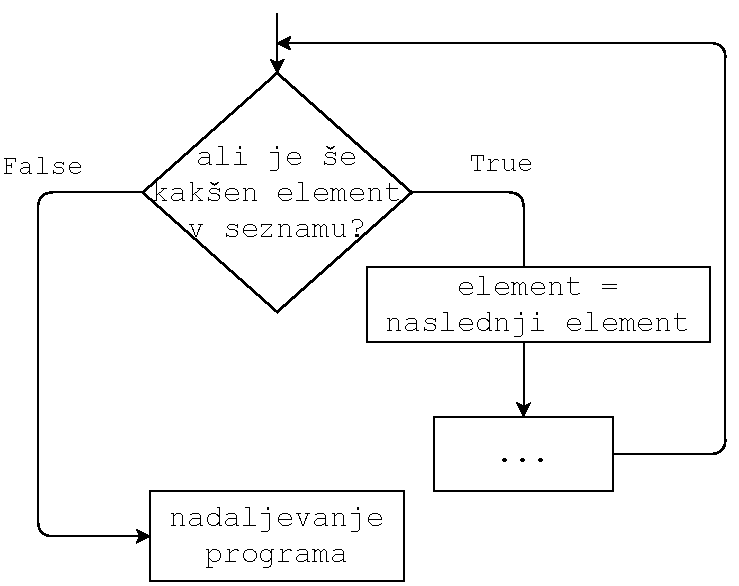
\includegraphics[width=0.5\linewidth]{img/for1.pdf}
    \caption{Potek izvedbe osnovne oblike zanke \texttt{for}.}
    \label{img:for1}
\end{figure}
Izvajanje zanke torej ponavljamo vse dokler je v seznamu (ali nizu) še kakšen element, pri čemer se spremenljivka \texttt{element} pomika od začetka proti koncu seznama (ali niza). Če bi npr. želeli izpisati vse elemente v seznamu, pri čemer bi vsak element izpisali v svoji vrstici, bi to lahko naredili takole:
\begin{lstlisting}[language=Python]
>>> seznam = [1,2,3]
>>> for element in seznam:
	print(element)
1
2
3
\end{lstlisting}
Na podoben način bi se lahko sprehodili tudi čez niz:
\begin{lstlisting}[language=Python]
>>> niz = "ABC"
>>> for znak in niz:
	print(znak)
A
B
C
\end{lstlisting}
V tem primeru se zanka \texttt{for} torej sprehaja čez znake niza.

Povadimo sprehajanje še na zgledu.
\begin{zgled}
Napiši program, ki od uporabnika preko funkcije \texttt{eval} prebere seznam in izpiše najmanjši element seznama (brez uporabe funkcije \texttt{min}). 
\end{zgled}
\begin{resitev}
Najmanjši element bomo našli tako, da se bomo z zanko \texttt{for} sprehodili čez seznam in si zapomnili element, ki je pač najmanjši. Kako pa vemo, da je nek element najmanjši, če ostalih še nismo pregledali? Težko. Vemo pa, če je nek element manjši od vseh elementov, ki smo jih pregledali preden smo do njega prišli. Nalogo lahko rešimo tako, da naredimo predpostavko, da je najmanjši ničti element v seznamu. Potem naredimo sprehod čez celoten seznam. Če bomo našli kakšen element, ki je manjši od trenutno najmanjšega, bomo trenutno najmanjši element postavili na tega, ki je očitno manjši. To bomo nadaljevali, dokler ne pridemo do konca seznama.
\begin{lstlisting}[language=Python,numbers=left]
seznam = eval(input("Vnesi seznam: "))

najmanjsi = seznam[0] # trenutno najmanjši

for element in seznam: # sprehod čez elemente
    if element < najmanjsi: # našli manjšega?
        najmanjsi = element # popravimo vrednost

print(najmanjsi)
\end{lstlisting}
Program sicer deluje pravilno, ampak bi ga lahko še nekoliko optimizirali. Trenutno namreč ničti element v seznamu pregledamo dvakrat. Sprehoda z zanko \texttt{for} nam torej ne bi bilo potrebno delati čez cel seznam, ampak bi ga lahko naredili čez rezino seznama, ki se začne na indeksu 1. Torej bi zanko \texttt{for} lahko delali čez rezino \texttt{seznam[1:]}.
\end{resitev}

\section{Sprehajanje s funkcijo \texttt{range} in sprehajanje čez indekse}

Z zanko \texttt{for} se lahko sprehajamo tudi čez sezname, ki jih generira funkcija \texttt{range}. Na tak način se lahko sprehajamo čez vrednosti elementov v določenem razponu. Vsa števila od 0 do vključno števila, ki ga je vnesel uporabnik, bi torej lahko izpisali tudi takole:
\begin{lstlisting}[language=Python]
n = int(input("Vnesi število: "))
for i in range(n+1):
    print(i)
\end{lstlisting}

Zanko \texttt{for} bi lahko na podoben način uporabili za sprehajanje po indeksih seznama. Indekse in vrednosti v seznamu na posameznih indeksih bi lahko izpisali takole:
\begin{lstlisting}[language=Python]
for i in range(len(seznam)):
    print(i, seznam[i])
\end{lstlisting}
Tokrat funkciji \texttt{range} kot argument \texttt{stop} podamo dolžino seznama, kar pomeni, da bo funkcija zgenerirala razpon elementov v intervalu od 0 do \texttt{len(seznam)-1}, kar je ravno razpon indeksov seznama. Tudi zato torej argument \texttt{stop} v interval ni vključen in zato funkcija \texttt{range} (tudi) deluje kakor deluje.

\section{Sprehajanje čez elemente ali čez indekse?}
Zgornji program bo poleg indeksa izpisal še vrednost elementa, ki se nahaja na posameznem indeksu. Ali bi lahko do indeksa elementov prišli tudi v primeru, ko se sprehajamo neposredno po elementih seznama? Težko. Zato v primeru, ko informacijo o indeksu potrebujemo, izvajamo zanko čez indekse in ne čez elemente.  

Poglejmo si spodnji primer, kjer rešitev zahteva izvedbo sprehoda čez indekse seznama.
\begin{zgled}
Napiši program, ki od uporabnika preko funkcije \texttt{eval} prebere seznam in izpiše najmanjši element seznama ter njegov indeks. 
\end{zgled}
\begin{resitev}
Najmanjši element bomo našli na podoben način kot prej, le da si moramo tokrat zapomniti tudi njegov indeks. Ker preko direktnega sprehoda čez elemente seznama informacije o indeksih elementov nimamo, se bomo morali sprehoditi čez indekse seznama.
\begin{lstlisting}[language=Python,numbers=left]
seznam = eval(input("Vnesi seznam: "))

najmanjsi = seznam[0] # trenutno najmanjši element
najmanjsi_i = 0 # zapomnimo si tudi njegov indeks

for i in range(len(seznam)): # sprehod čez indekse
    element = seznam[i] # preko indeksa do elementa
    if element < najmanjsi: # našli manjšega?
        najmanjsi = element # popravimo vrednost
        najmanjsi_i = i # popravimo indeks

print(najmanjsi)
print(najmanjsi_i)
\end{lstlisting}
Spet bi lahko pri sprehodu prvi element seznama izpustili, tako da bi se sprehajali čez razpon indeksov \texttt{range(1, len(seznam))}.
\end{resitev}

Zgornja rešitev ima manjšo pomanjkljivost, in sicer ne upošteva, da se lahko enako majhen element v seznamu pojavi večkrat. V tem primeru vrne zgolj indeks njegove prve pojavitve. Naprednejšo rešitev prikazuje spodnji zgled.

\begin{zgled}
Napiši program, ki od uporabnika preko funkcije \texttt{eval} prebere seznam in izpiše najmanjši element seznama ter vse indekse njegove pojavitve. 
\end{zgled}
\begin{resitev}
Rešitev bo podobna kot prej, le da si bomo indekse pojavitve najmanjšega elementa zabeležili kar v seznam. V primeru, da bomo našli manjši element od trenutnega, bomo naredili nov seznam, ki bo vseboval samo en indeks (trenutni indeks). V primeru, da bomo našli element, ki bo enak trenutno najmanjšemu, bomo v seznam indeksov dodali trenutni indeks. V prejšnjih dveh zgledih smo na koncu omenili boljšo rešitev, ki pri sprehodu izpusti ničti element seznama, saj smo tega upoštevali že pred zanko. Tokrat bo program brez te "optimizacije" deloval narobe. V primeru, da bo najmanjši element na ničtem mestu, bo njegov indeks v seznamu najmanjših indeksov namreč nastopal dvakrat.
\begin{lstlisting}[language=Python,numbers=left]
seznam = eval(input("Vnesi seznam: "))

najmanjsi = seznam[0] # trenutno najmanjši element
najmanjsi_i = [0] # v seznam shranimo njegov indeks

# sprehod čez indekse (ničti element izpustimo)
for i in range(1, len(seznam)): 
    element = seznam[i] # preko indeksa do elementa
    if element < najmanjsi: # našli manjšega?
        najmanjsi = element # popravimo vrednost
        najmanjsi_i = [i] # resetiramo seznam indeksov
    elif element == najmanjsi: # našli enako majhnega
        najmanjsi_i.append(i) # dodamo indeks

print(najmanjsi)
print(najmanjsi_i)
\end{lstlisting}
\end{resitev}

\section{Spreminjanje elementov seznama z zanko \texttt{for}}
Kaj pa v primeru da želimo seznam v zanki spremeniti, npr. da želimo vse negativne vrednosti seznama spremeniti v pozitivne (izračunati želimo absolutne vrednosti elementov seznama in seznam skladno s tem posodobiti). Žal funkcije \texttt{abs} nad seznamom ne moremo pognati (napaka), zato moramo izračunati absolutno vrednost vsakega elementa posebej, pri čemer lahko to rešimo z uporabo zanke \texttt{for}. Poskusimo z običajnim sprehodom čez elemente seznama.
\begin{lstlisting}[language=Python]
>>> seznam = [-1, 10, -5, 15, 0, -3]
>>> for element in seznam:
	element = abs(element)
	print(element)
1
10
5
15
0
3
>>> print(seznam)
[-1, 10, -5, 15, 0, -3]
\end{lstlisting}
Elemente smo torej uspešno postavili na njihove absolutne vrednosti, na kar nakazujejo izpisi, ki smo jih izvedli v telesu zanke. Kot pa vidimo iz izpisa, ki je sledil zanki, se seznam ni spremenil, saj še vedno vsebuje negativne elemente. V konkretnem primeru torej samega seznama nismo spreminjali. Če bi želeli spreminjati seznam, bi to lahko naredili preko indeksiranja:
\begin{lstlisting}[language=Python]
>>> seznam = [-1, 10, -5, 15, 0, -3]
>>> for i in range(len(seznam)):
	seznam[i] = abs(seznam[i])
	print(seznam[i])
1
10
5
15
0
3
>>> print(seznam)
[1, 10, 5, 15, 0, 3]
\end{lstlisting}
Zdaj se je seznam seveda spremenil, saj smo absolutne vrednosti direktno prirejali seznamu na posameznem indeksu.

\section{Zanka \texttt{for} ali zanka \texttt{while}?}
Vidimo, da so naši programi z uporabo zanke \texttt{for} v določenih veliko krajši in lepši kot v primeru uporabe zanke \texttt{while}. Poleg tega nam pri uporabi zanke \texttt{for} ni potrebno skrbeti, da bo program za vedno obtičal v zanki (mrtva zanka). Zakaj bi torej sploh uporabljali zanko \texttt{while}? Izkaže se, da je zanka \texttt{while} bolj splošna kot zanka \texttt{for} in da lahko z njo rešimo določene probleme, ki jih z zanko \texttt{for} ne moremo. Kako bi npr. z zanko \texttt{for} od sodnika smučarskih skokov brali dolžine skokov, dokler sodnik ne vnese števila 0? Koliko ponovitev bi morali narediti? Kako bi z zanko \texttt{for} odštevali manjše število od večjega, dokler števili ne bi postali enaki? Odgovor je enostaven. Težko.

Vprašajmo se, kaj je skupnega primerom, kjer zanka \texttt{for} odpove. V obeh zgornjih primerih je število ponovitev, ki jih bo morala zanka narediti, vnaprej težko predvidljivo. V splošnem velja, da zanko \texttt{while} uporabljamo, kadar število ponovitev zanke težko podamo vnaprej, lahko pa oblikujemo pogoj, ki bo določil, do kdaj naj se zanka izvaja. V primeru, da je število ponovitev predvidljivo (npr. podan je razpon štetja ali pa seznam s fiksno dolžino, čez katerega se sprehajao) pa je kot nalašč zanka \texttt{for}.

\section{Stavek \texttt{break}}

V kombinaciji z zanko \texttt{for} lahko prav tako kot pri zanki \texttt{while} uporabljamo stavek \texttt{break}. Ta izvajanje zanke prekine, kljub temu, da ta še ni prišla do konca seznama (ali česa drugega). Primer uporabe stavka \texttt{break} znotraj zanke \texttt{for} ponazarja spodnja koda:
\begin{lstlisting}[language=Python]
for element in seznam:
    # telo zanke
    ...
    if dodaten_pogoj: 
        break # prekine izvajanje zanke
# nadaljevanje programa
...
\end{lstlisting}
Potek izvedbe kode iz primera prikazuje slika \ref{img:for2}.
\begin{figure}
    \centering
    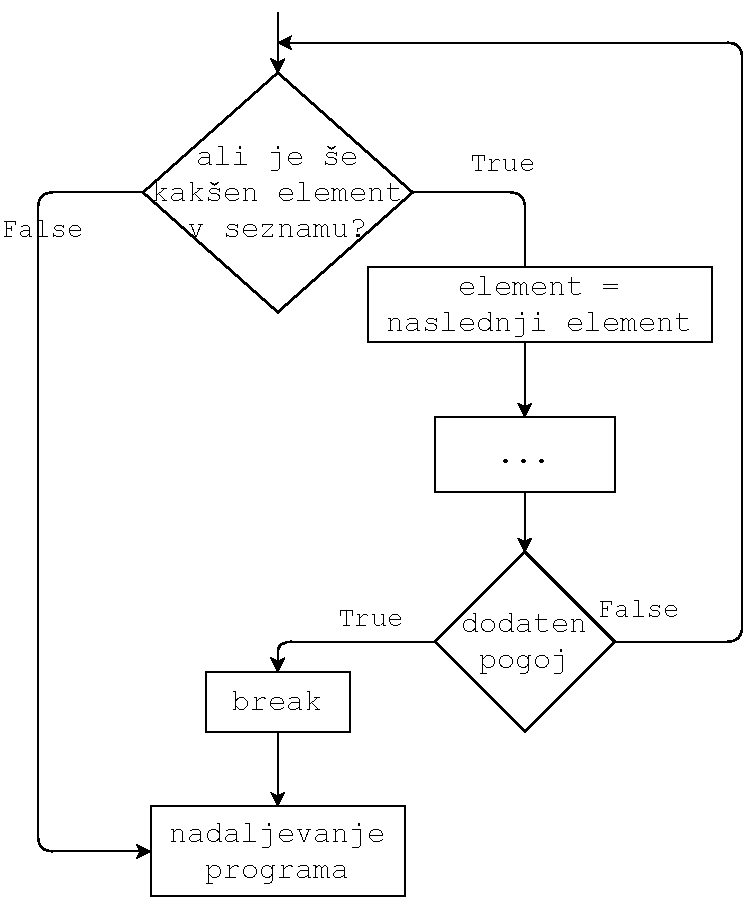
\includegraphics[width=0.5\linewidth]{img/for2.pdf}
    \caption{Potek izvedbe zanke \texttt{for} v kombinaciji s stavkom \texttt{break}.}
    \label{img:for2}
\end{figure}


\section{Veja \texttt{else}}

Podobno kot lahko vejo \texttt{else} kombiniramo z zanko \texttt{while}, jo lahko kombiniramo tudi z zanko \texttt{for}:
\begin{lstlisting}[language=Python]
for element in seznam:
    # telo zanke
    ...
    if dodaten_pogoj:
        break # prekini izvajanje zanke
else: # samo če zanka ni bila prekinjena z break
    # konec seznama
    ...
# nadaljevanje programa
...
\end{lstlisting}

Veja \texttt{else} se bo kot pri zanki \texttt{while} izvedla samo v primeru, ko zanka ni bila prekinjena s stavkom \texttt{break}. Demonstrirajmo uporabo koncepta na zgledu s tujimi števili.

\begin{zgled}
Napiši program, ki od uporabnika prebere dve celi števili in izpiše, če sta števili tuji. Števili sta tuji, če nimata nobenega skupnega delitelja, ki je večji od 1.
\end{zgled}
\begin{resitev}
Program bo strukturiran zelo podobno kot v primeru zanke \texttt{while}, le da bomo tokrat razpon števil, čez katera se sprehaja kandidat, ustvarili z uporabo funkcije \texttt{range}. 

\begin{lstlisting}[language=Python,numbers=left]
st1 = int(input("Vnesi prvo število: "))
st2 = int(input("Vnesi drugo število: "))

# sprehod od 2 do manjšega od obeh števil
# desni del intervala naj bo vključen,
# zato prištejemo 1
for delitelj in range(2,min(st1, st2)+1):
    # ali delitelj deli obe števili?
    if st1 % delitelj == 0 and st2 % delitelj == 0:
        print("Števili nista tuji")
        break # lahko prenehamo z iskanjem
else: # ali se je zanka odvrtela do konca
    # zanke nismo prekinili s stavkom break
    print("Števili sta tuji")
\end{lstlisting}
\end{resitev}


\section{Gnezdenje zank}

Podobno kot smo gnezdili stavke \texttt{if} lahko gnezidmo tudi zanke. To pomeni, da bomo zanko izvajali znotraj druge zanke. Primer gnezdenja zanke \texttt{for} prikazuje spodnji izsek kode:
\begin{lstlisting}[language=Python]
>>> for i in range(5):
        for j in range(5):
            print(i,j)
0 0
0 1
0 2
0 3
0 4
1 0
1 1
...
3 3
3 4
4 0
4 1
4 2
4 3
4 4
\end{lstlisting}
Notraja zanka \texttt{for} torej za vsako iteracijo zunanje zanke izvede enako število ponovitev.

Potrenirajmo na zgledu.

\begin{zgled}
Napiši program, ki od uporabnika prebere celo število in izpiše poštevanko števil od 1 do vključno podanega števila.
\end{zgled}
\begin{resitev}
Števila od 1 do podanega števila \texttt{n} bomo najprej množili z 1, potem z 2, potem s 3 in tako naprej, dokler ne pridemo do števila \texttt{n}. To lahko enostavno rešimo z uporaba ugnezdene zanke.
\begin{lstlisting}[language=Python]
n = int(input("Vnesi število: "))

for i in range(1, n+1): # zunanja zanka
    for j in range(1, n+1): # notranja zanka
        print(i*j) # izpis produkta
    print() #nova vrstica
\end{lstlisting}
V primeru, da uporabnik vpiše število 3, bo izpis sledeč:
\begin{lstlisting}[language=Python]
1
2
3

2
4
6

3
6
9
\end{lstlisting}
\end{resitev}

V zgornjih primerih je bila notranja zanka neodvisna od tega, kako daleč se je že odvila zunanja zanka. Ponavadi pa temu ni tako. Primer ugnezdene zanke, pri kateri je razpon notranje zanke odvisen od števila izvedenih iteracij zunanje zanke, prikazuje spodnji izsek kode:
\begin{lstlisting}[language=Python]
>>> for i in range(5):
        for j in range(i,5):
            print(i,j)
0 0
0 1
0 2
0 3
0 4
1 1
1 2
1 3
1 4
2 2
2 3
2 4
3 3
3 4
4 4
\end{lstlisting}
V prvi iteraciji zunanje zanke, se torej notranja zanka izvede petkrat, v drugi štirikrat, v tretji trikrat, v četrti dvakrat, v peti pa zgolj enkrat. Kasnejša kot je iteracija zunanje zanke, manjše je število ponovitev ugnezdene zanke. 

Povadimo tako gnezdenje še na primeru s tujimi števili.
\begin{zgled}
Napiši program, ki od uporabnika prebere celo število in izpiše vsa števila, ki so podanemu številu tuja in so od njega manjša. 
\end{zgled}
\begin{resitev}
Kandidati, ki jih moramo torej obravnavati, se gibljejo v razponu od števila 1 (ki je vsem številom tuje število) do števila \texttt{n-1}, pri čemer je \texttt{n} število, ki ga je vnesel uporabnik. Kako za posameznega kandidata preverimo, če je tuj številu \texttt{n}? Podobno kot prej -- tako da se sprehodimo od števila 2, do manjšega od obeh števil. Če smo našli kakšnega delitelja, si števili očitno nista tuji.
\begin{lstlisting}[language=Python,numbers=left]
n = int(input("Vnesi število: "))

for kandidat in range(1, n): # razpon cez kandidate
    # kandidat ne sme imeti nobenega skupnega delitelja
    # ugnezdimo kodo iz prejšnjih zgledov
    st1 = n
    st2 = kandidat
    
    # sprehod od 2 do manjšega od obeh števil
    # desni del intervala naj bo vključen, zato prištejemo 1
    for delitelj in range(2,min(st1, st2)+1):
        # ali delitelj deli obe števili?
        if st1 % delitelj == 0 and st2 % delitelj == 0:
            break # lahko prekinemo ugnezdeno zanko
    else: # ali se je ugnezdena zanka odvrtela do konca
        # ugnezdene zanke nismo prekinili s stavkom break
        print(kandidat)
\end{lstlisting}
\end{resitev}
Ugnezdena zanka je v tem primeru odvisna od tega kako daleč je naš program prišel z zunanjo zanko. Mimogrede, na podoben način bi lahko gnezdili tudi zanko \texttt{while}. 


\section{Izbirni argumenti funkcij in izbirni argumenti funkcije \texttt{print}}

Tole sicer ni neposredno povezano z zanko \texttt{for}, bo pa služilo kot osnova za dopolnitev zgleda s poštevanko. 

Povedali smo že, da funkcije sprejemajo argumente, ki jih ob klicu pač podamo. V določenih primerih pa imajo funkcije tudi t.i. \emph{izbirne} ali \emph{opcijske} argumente, za katere velja da imajo (pred)nastavljeno \emph{privzeto} vrednost. V primeru, da vrednosti teh argumentov eksplicitno ne podamo, bodo ti nastavljeni na njihove privzete vrednosti. V primeru, da vrednosti tem argumentom podamo, bomo s tem \emph{povozili} privzete vrednosti in uporabljene bodo podane (naše) vrednosti.

Poglejmo si dva izbirna argumenta funkcije \texttt{print} in primer njune uporabe. Do dokumentacije funkcije \texttt{print} lahko pridemo preko funkcije \texttt{help}:
\begin{lstlisting}[language=Python]
>>> help(print)
Help on built-in function print in module builtins:

print(...)
    print(value, ..., sep=' ', end='\n', file=sys.stdout, 
    flush=False)
    
    Prints the values to a stream, or to sys.stdout by default.
    Optional keyword arguments:
    file:  a file-like object (stream); defaults to the current 
    sys.stdout.
    sep:   string inserted between values, default a space.
    end:   string appended after the last value, default a newline.
    flush: whether to forcibly flush the stream.
\end{lstlisting}
Zaenkrat nas bosta zanimala predvsem argumenta \texttt{sep} in \texttt{end}. Funkcija \texttt{print} deluje tako, da sprejme poljubno število številk, nizov in še česa drugega, to med seboj združi in izpiše na zaslon. Pri tem argument \texttt{sep} določa, s čim naj podane številke, nize in še kaj drugega med seboj združi. Privzeto je ta argument postavljen na vrednost \texttt{' '}, kar vidimo iz zgleda klica funkcije (\texttt{sep=' '}). To pomeni, da bo izpis narejen tako, da bodo med podanimi argumenti za izpis vstavljeni presledki. Povadimo:
\begin{lstlisting}[language=Python]
>>> print(1,2,3) # privzeta vrednost argumenta
1 2 3
>>> print(1,2,3, sep='') # brez presledka
123
>>>print(1,2,3, sep='+++') # poljuben niz kot ločilo
1+++2+++3
\end{lstlisting}
Izbirni argument \texttt{end} podaja niz, ki naj se vstavi na koncu izpisa. Privzeto je argument \texttt{end} nastavljen na znak \texttt{'$\backslash$n'} (\texttt{end='$\backslash$n'}), ki predstavlja znak za novo vrstico \angl{line feed}. Tudi tega lahko postavimo na kakšno drugo vrednost. 

Povadimo nastavljanje opcijskih argumentov na zgledu v kombinaciji z ugnezdeno zanko \texttt{for}.

\begin{zgled}
Napiši program, ki od uporabnika prebere celo število in izpiše poštevanko števil od 1 do vključno podanega števila. Pri tem naj bo poštevanka s posameznim številom podana v svoji vrstici, števila pa naj bodo ločena s presledki.
\end{zgled}
\begin{resitev}
Rešitev bo podobna kot prej, le da se tokrat ne bomo pomikali v novo vrstico po vsakem izpisu. To lahko naredimo tako, da opcijski argument  \texttt{end} nastavimo na znak \texttt{' '}.

\begin{lstlisting}[language=Python]
n = int(input("Vnesi število: "))

for i in range(1, n+1): # zunanja zanka
    for j in range(1, n+1): # notranja zanka
        print(i*j, end = ' ') # izpis produkta brez nove vrstice
    print() #nova vrstica
\end{lstlisting}
V primeru, da uporabnik vpiše število 3, bo tokrat izpis sledeč:
\begin{lstlisting}[language=Python]
1 2 3
2 4 6
3 6 9
\end{lstlisting}
\end{resitev}

\chapter{Uporaba in pisanje funkcij}
\section{Kaj so funkcije in zakaj so uporabne?}
Kot že vemo, funkcije predstavljajo del kode, ki jo lahko izvedemo tako, da funkcijo preprosto pokličemo. 

Uporaba funkcij ima veliko prednosti. Govorili smo že o tem, da je glavno vodilo programiranja razdelitev problemov na obvladljive podprobleme. Določanje algoritma, ki ga potem samo še prenesemo v programsko kodo, je podobno določanju recepta, ki ga potem prenesemo v okusno jed. Prav tako, kot se moramo pri kuhanju zavedati sestavin, ki jih imamo na razpolago, se moramo tudi pri programiranju zavedati gradnikov programskega jezika, ki jih lahko pri pisanju algoritma uporabimo. 

Funkcije nam omogočajo, da osnovne korake za reševanje programa vgradimo v enostavnejše funkcije, enostavnejše funkcije v kompleksnejše in tako naprej. Podobno, kot če bi pri peki torte lahko uporabili že vnparej pripravljeno testo, preliv in kar se pri torti še uporabi, namesto da moramo torto sestaviti iz enostavnejših (nižjenivojskih) sestavin, kot so jajca, mleko in sladkor. Tako, kot bi lahko tudi pri peki seveda šli v drug ekstrem in se lotili reje kokoši, bi na veliko nižji nivo lahko šli tudi pri programiranju, ampak pustimo to za kdaj drugič. S pisanjem svojih funkcij se lahko torej najprej lotimo enostavnejših korakov, ki predstavljajo del rešitve izbranega problema. Potem lahko vmesne rešitve (velikokrat na enostaven način) združimo v končno rešitev. Če bi npr. želeli najti vsa praštevila v določenem razponu števil, bi lahko najprej napisali funkcijo, ki za podano število preveri, če je praštevilo. Vse kar bi morali narediti potem bi bil zgolj klic te funkcije za vsako število z intervala.

Zgled s praštevili pa nam je posredno razodel še eno veliko prednost uporabe funkcij. Isto kodo, tj. preverjanje ali je neko število praštevilo, bomo poklicali večkrat, vsakič seveda z drugim argumentom, tj. številom, ki je kandidat za praštevilo. Funkcije nam torej omogočajo tudi to, da lahko isti kos kode večkrat pokličemo brez tega, da bi jo vključevali v zanke ali pa kopirali v vse dele programa, kjer jo potrebujemo. 

To kodo bi lahko delili tudi z drugimi programerji. Če smo npr. napisali zelo dobro funkcijo za iskanje praštevil in smo nad njo nadvse navdušeni, hkrati pa vemo, da bi bila lahko koristna tudi za druge iskalce praštevil, lahko funkcijo enostavno zapakiramo v t.~i. modul, ki ga objavimo na internetu. 

\section{Kako definiramo funkcijo?}

Vsaki funkciji, ki jo želimo v naših programih ponovno uporabiti, moramo dati seveda neko ime, preko katerega jo bomo lahko po potrebi poklicali. Skupaj s seznamom argumentov, ki jih bo naša funkcija sprejela, to podamo v definiciji funkcije. Definicijo funkcije začnemo z rezervirano besedo \texttt{def} in končamo z dvopičjem:

\begin{lstlisting}[language=Python]
def ime_funkcije(argument_1, argument_2,..., argument_n):
\end{lstlisting}

Definiciji funkcije sledi njena vsebina. Stavke, ki so v funkciji vsebovani tudi tokrat določimo z zamikanjem na začetku vrstice (podobno kot pri pogojnemu stavku in zankah). Ko želimo Pythonu sporočiti, da koda ni več del funkcije, enostavno nehamo zamikati.

Spodnji primer predstavlja definicijo enostavne funkcije, ki sešteje vrednosti dveh spremenljivk (\texttt{a} in \texttt{b}) v novo spremenljivko (\texttt{c}) in rezultat seštevanja izpiše.
\begin{lstlisting}[language=Python,numbers=left]
def sestej(a, b):
    c = a + b
    print(c)
    # tale komentar je še del funkcije
# tale komentar ni več del funkcije
\end{lstlisting}

Kaj pa se zgodi, ko program s tole definicijo poženemo. Navidez se ne zgodi nič, če pa v ukazno vrstico napišemo ime pravkar definirane funkcije, bi moral Python izpisati nekaj podobnega temu:
\begin{lstlisting}[language=Python]
<function sestej at 0x000001C24E1481E0>
\end{lstlisting}
Kaj to pomeni? To pomeni, da se je v našem \emph{imenskem prostoru} (pojem bomo razložili v kratkem) pojavilo ime \texttt{sestej}, ki ima v ozadju funkcijo, ta pa je shranjena nekje v pommnilniku (natančneje na pomnilniškem naslovu \texttt{0x000001C24E1481E0}). Ko smo izvedli zgornjo kodo, smo torej dobili definicijo funkcije \texttt{sestej}, ki jo zdaj lahko pokličemo.

Do zdaj smo funkcije vedno klicali tako, da so imenu funkcije sledili oklepaji, znotraj katerih smo našteli vrednosti argumentov, nad katerimi smo želeli funkcijo poklicati. In seveda je tako tudi v primeru funkcij, ki jih definiramo sami. Če bi torej želeli izpisati vsoto števil 5 in 7, bi lahko izvedli klic
\begin{lstlisting}[language=Python]
>>>sestej(5,7)
12
\end{lstlisting}

Ko smo funkcijo definirali se torej koda znotraj funkcije sploh ni izvedla. Izvedla se je zgolj njena definicija, ki nam je njeno ime umestila v imenski prostor (podobno, kot če smo nekemu imenu -- sprememnljivki, priredili neko vrednost). Dejanska izvedba stavkov znotraj funkcije pa se je izvršila šele, ko smo funkcijo poklicali. Mimogrede, če bi v funkciji imeli napako, kot je npr. uporaba nedefinirane spremenljivke, bi jo Python našel šele ob klicu funkcije.

\section{Globalni imenski prostor}
Vsakič, ko v Pythonu definiramo novo spremenljivko, se ime, preko katerega bomo dostopali do vrednosti te spremenljivke, shrani v t.~i. \emph{imenski prostor}. Podobno se zgodi ob definiciji funkcije, le da se v tem primeru za imenom funkcije skriva vsebina funkcije, ki se bo izvedla, ko jo bomo poklicali. Ko npr. definiramo spremenljivki \texttt{x} in \texttt{y} z uporabo kode
\begin{lstlisting}[language=Python]
>>> x = 5
>>> y = 7
\end{lstlisting}
se v imenskem prostoru pojavita imeni \texttt{x} in \texttt{y}, za katerimi se skrivata podani vrednosti, kot prikazuje slika \ref{img:imenski_prostor_1}.
\begin{figure}
    
\includegraphics[width=\linewidth]{img/imenski_prostor.pdf}
    \caption{Imena v imenskem prostoru kažejo na konkretne vrednosti v pomnilniku.}
    \label{img:imenski_prostor_1}
\end{figure}
Preko imen \texttt{x} in \texttt{y} lahko zdaj dostopamo do vrednosti, ki se skrivajo v ozadju, ne da bi se morali zavedati kje konkretno v pomnilniku so te vrednosti shranjene, kar nam bistveno olajša življenje.

Definicije novih imen, pa naj gre za imena spremenljivk ali funkcij, ki jih ustvarimo izven funkcij, se shranijo v t.~i. \emph{globalni imenski prostor}. Zato tem imenom pogosto rečemo kar globalna imena, spremenljivkam pa \emph{globalne spremenljivke}. Če obstaja globalni imenski prostor pa bo verjetno obstajal tudi lokalni. Poglejmo si, kaj se zgodi, ko funkcijo pokličemo.

\section{Kaj se zgodi ob klicu funkcije in lokalni imenski prostor}
Kot smo že omenili, se ob definiciji funkcije v globalnem imenskem prostoru ustvari novo ime, ki je enako imenu funkcije. To kaže na samo funkcijo, tako da bomo lahko le-to kasneje preko imena tudi poklicali. Situacijo po definiciji funkcije \texttt{sestej} prikazuje slika \ref{img:imenski_prostor_2}. \begin{figure}
    
\includegraphics[width=\linewidth]{img/imenski_prostor_2.pdf}
    \caption{Ob definiciji funkcije v imenskem prostoru dobimo novo ime, ki je enako imenu funkcije. Za tem imenom se skriva naša funkcija.}
    \label{img:imenski_prostor_2}
\end{figure}

Dopolnimo program, v katerem smo napisali funkcijo \texttt{sestej}, še z njenim klicem.
\begin{lstlisting}[language=Python,numbers=left]
def sestej(a, b): # definicija funkcije
    c = a + b
    print(c)
x = 5
y = 7
sestej(x,y) # klic funkcije
\end{lstlisting}
Vrstice programa od 1, 4 in 5 bi morale biti zdaj že popolnoma jasne. Kaj pa se zgodi, ko program pride do vrstice 6? Ustvari se lokalni imenski prostor funkcije \texttt{sestej}, znotraj katerega bo funkcija ustvarila svoje lokalne spremenljivke. V lokalnem imenskem prostoru se najprej ustvarita lokalni spremenljivki z imeni \texttt{a} in \texttt{b}, katerima se priredita vrednosti spremenljivk \texttt{x} in {y}, tj. spremenljivk, s katerimi smo funkcijo poklicali. Enako posledico bi imela prireditev
\begin{lstlisting}[language=Python]
>>> a = x
>>> b = y
\end{lstlisting}
s to razliko, da bi se imeni \texttt{a} in \texttt{b} ustvarili v globalnem imenskem prostoru.

Prirejanje vrednosti ene spremenljivki drugi pa je v jeziku Python nekoliko poenostavljeno. Vrednost, ki je že shranjena v pomnilniku v tem primeru namreč zgolj dobi dodatno ime, brez da bi se dejansko kopirala, s čimer smo s pomnilniškim prostorom veliko bolj varčni. Imeni si torej delita isti objekt v pomnilniku. O tem bomo še govorili, zaenkrat pa se vrnimo k naši funkciji in njenem lokalnem imenskem prostoru. Situacijo ob klicu funkcije prikazuje slika \ref{img:imenski_prostor_3}.
\begin{figure}
    \centering
    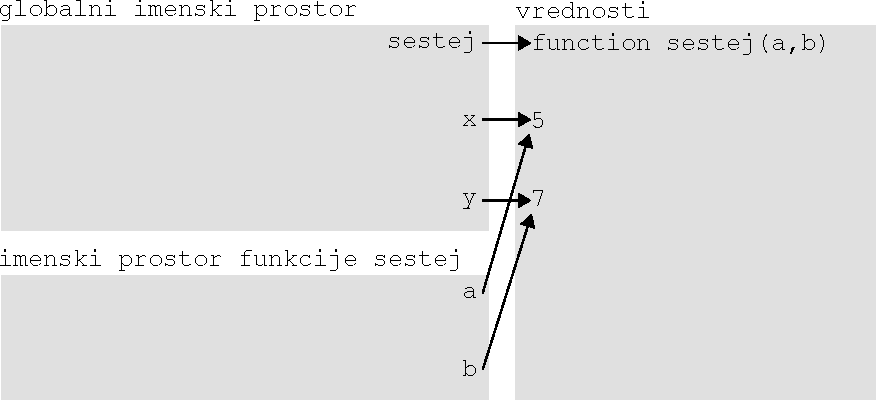
\includegraphics[width=\linewidth]{img/imenski_prostor_3.pdf}
    \caption{Ob klicu funkcije se ustvari njen lokalni imenski prostor znotraj katerega se ustvarijo lokalna imena, ki kažejo na vrednosti, s katerimi smo funkcijo poklicali.}
    \label{img:imenski_prostor_3}
\end{figure}

Vsa imena, ki jih bomo v nadaljevanju definirali znotraj funkcije, bodo ustvarjena v lokalnem imenskem prostoru funkcije. Ko naš program na primer izvede vrstico 2 (ta se je ob definiciji funkcije preskočila in se izvede šele ob njenem klicu), bo prišlo do situacije, kot jo prikazuje slika \ref{img:imenski_prostor_4}
\begin{figure}
    \centering
    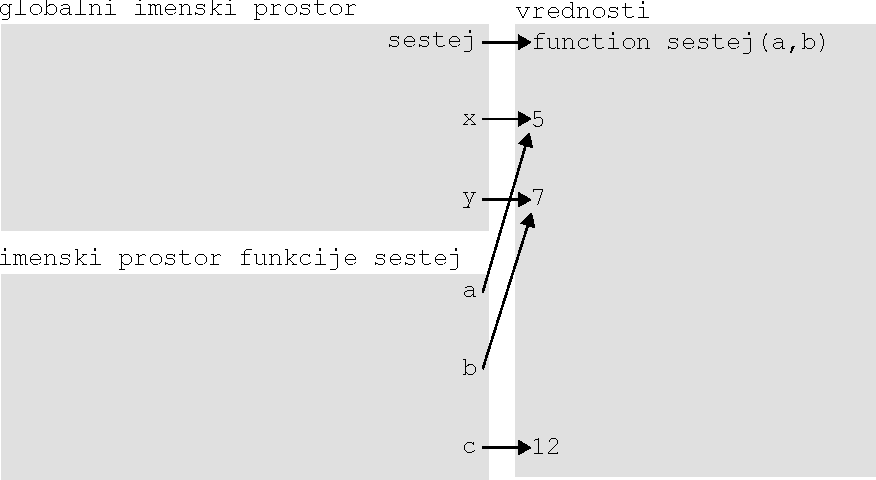
\includegraphics[width=\linewidth]{img/imenski_prostor_4.pdf}
    \caption{Vsa imena, ki jih definiramo znotraj funkcije, se ustvarijo zgolj v lokalnem imenskem prostoru te funkcije.}
    \label{img:imenski_prostor_4}
\end{figure}

Kaj pa bi se zgodilo, če bi znotraj funkcije definirali ime, ki obstaja že v globalnem imenskem prostoru. Nič posebnega. Spremenljivka s tem imenom bi se ustvarila v lokalnem imenskem prostoru funkcije in to na globalno spremenljivko ne bi vplivalo. Zgodilo bi se nekaj takega kot prikazuje slika \ref{img:imenski_prostor_5}.
\begin{figure}
    \centering
    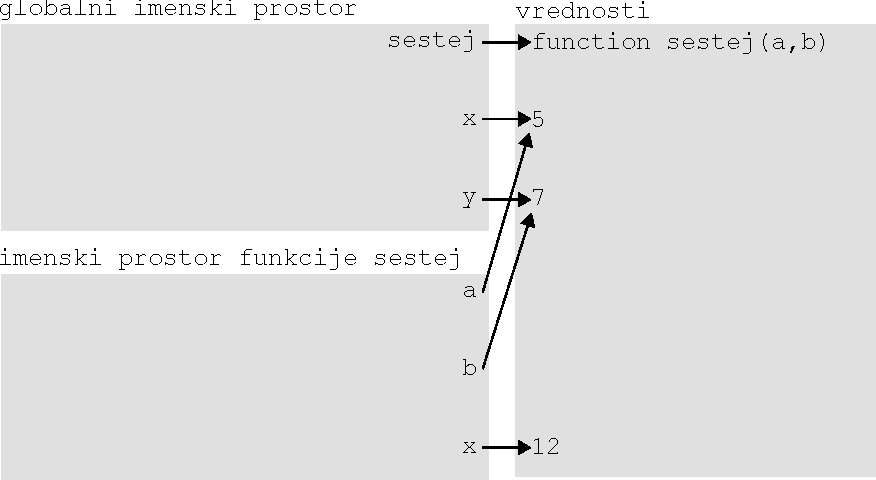
\includegraphics[width=\linewidth]{img/imenski_prostor_5.pdf}
    \caption{Znotraj funkcije lahko uporabljamo enaka imena spremenljivk kot izven funkcije in s tem ne vplivamo na globalne spremenljivke.}
    \label{img:imenski_prostor_5}
\end{figure}

Zakaj je tak način delovanja dober? Če bi morali znotraj funkcij paziti, da ne uporabljamo enakih imen, kot so že definirana izven funkcij, potem bi morali že vnaprej predvideti kakšna imena bodo pri programiranju uporabljali vsi bodoči uporabniki naših funkcij. Prav tako bi morali biti zelo pazljivi, ko bi obstoječe funkcije uporabljali mi. Vedeti bi morali katere spremenljivke za izpis nečesa na zaslon na primer uporablja funkcija \texttt{print}. Tem imenom bi se morali izogibati, kar pa bi bilo skrajno nerodno in nesmiselno.

Vprašanje, na katerega moramo še odgovoriti je, kaj se zgodi, ko se funkcija izvede do konca. V našem primeru se funkcija konča po izpisu vrednosti spremenljivke \texttt{c} (vrstica 3). Ko se funkcija konča, njenega lokalnega imenskega prostora ne potrebujemo več. Če bomo funkcijo še enkrat poklicali, bo Python ustvaril nov lokalen imenski prostor. Iz tega razloga po končanju izvedbe funkcije lokalni imenski prostor funkcije izgine. V našem konkretnem primeru torej imena \texttt{a}, \texttt{b} in \texttt{c} izginejo. Kaj pa vrednosti? Do vrednosti 12 ne moremo več dostopati preko nobene spremenljivke, zato se lahko izbriše tudi ta. Vrednosti 5 in 7 po drugi strani ostaneta, saj nanju še vedno kažeta imeni \texttt{x} in \texttt{y}. To prikazuje slika \ref{img:imenski_prostor_6}.
\begin{figure}
    \centering
    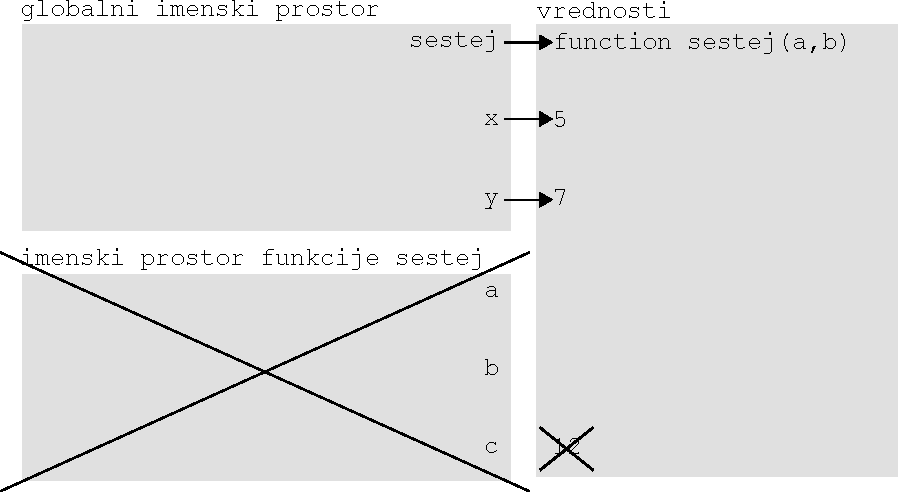
\includegraphics[width=\linewidth]{img/imenski_prostor_6.pdf}
    \caption{Po izvedbi klica funkcije, se njen imenski prostor izbriše.}
    \label{img:imenski_prostor_6}
\end{figure}

Iz globalnega imenskega prostora do lokalnih imenskih prostorov uporabljenih funkcij torej ne moremo dostopati, saj se po zaključku izvajanja funkcij (ko izvedba programa preide spet v globalni imenski prostor), lokalni imenski prostori izbrišejo. Kaj pa obratno? Iz lokalnega imenskega prostora funkcije, lahko dostopamo do globalnega (tudi zato se mu reče globalni), kar pomeni, da lahko dostopamo do vrednosti globalnih spremenljivk. Še pomembneje pa je to, da lahko iz lokalnega imenskega prostora funkcij, dostopamo do imen globalno definiranih funkcij. To pomeni, da lahko iz posamezne funkcije pokličemo druge funkcije (gnezdenje funkcij) ali pa tudi samo sebe. Slednjemu se reče \emph{rekurzija}, ampak pustimo to za kdaj drugič. 

Napišimo malo razširjen program, ki bo seštel vrednosti dveh seznamov. Pri tem si bomo pomagali z definicijo dveh funkcij.
\begin{lstlisting}[language=Python,numbers=left]
def sestej(a, b): # seštej in izpiši
    c = a + b
    print(c)

def sestej_seznama(a,b): # seštej istoležne elemente
    for i in range(len(a)):
        sestej(a[i], b[i])

sestej_seznama([1,2,3],[4,5,6]) # klic funkcije
\end{lstlisting}
Iz funkcije \texttt{sestej\_seznama} torej kličemo funkcijo \texttt{sestej}. Ali je to dovoljeno? Seveda. Imeni \texttt{sestej} in \texttt{sestej\_seznama} bomo po izvedbi vrstic 1 in 5 imeli v globalnem imenskem prostoru, kot prikazuje slika  \ref{img:imenski_prostor_7}.
\begin{figure}
    \centering
    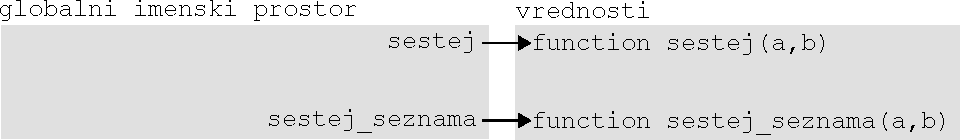
\includegraphics[width=\linewidth]{img/imenski_prostor_7.pdf}
    \caption{Imeni definiranih funkcij sta shranjeni v globalnem imenskem prostoru, zato jih lahko pokličemo od kjerkoli.}
    \label{img:imenski_prostor_7}
\end{figure}

Ker je globalni imenski prostor viden tudi iz lokalnih imenskih prostorov posameznih funkcij, jih lahko od tam tudi pokličemo. V sled temu je zgornji program popolnoma pravilen. 

Če program pogledamo podrobneje, lahko vidimo, da obe funkciji uporabljata enaka imena spremenljivk. Tudi to ne bo povzročalo nobenih težav, saj bo vsaka funkcija dobila svoj lasten lokalni imenski prostor. Ko bomo poklicali funkcijo \texttt{sestej\_seznama}, bo ta dobila lokalen imenski prostor. Ko bomo iz te funkcije poklicali funkcijo \texttt{sestej}, bo ta dobila svoj imenski prostor, ki se s prostorom funkcije \texttt{sestej\_seznama} ne bo prekrival. Lokalne imenske prostore si torej lahko predstavljamo kot ločene mehurčke, ki se med seboj ne prekrivajo. Stanje našega programa ob prvi izvedbi funkcije \texttt{sestej} do vključno vrstice 2 prikazuje slika \ref{img:imenski_prostor_8}.
\begin{figure}
    \centering
    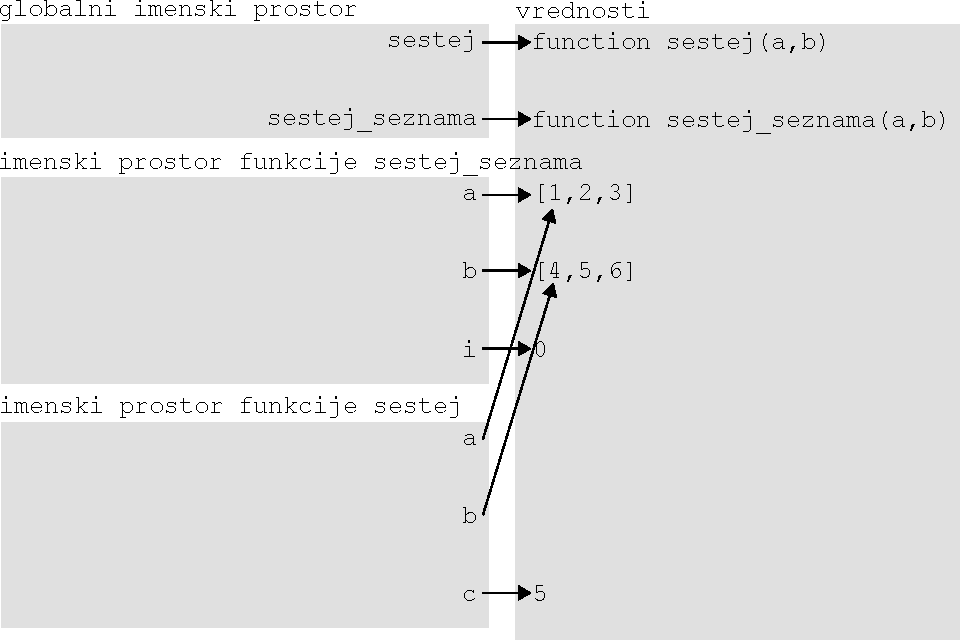
\includegraphics[width=\linewidth]{img/imenski_prostor_8.pdf}
    \caption{Lokalni imenski prostori funkcij so med seboj ločeni.}
    \label{img:imenski_prostor_8}
\end{figure}

Vprašanje za razmislek -- zakaj se znotraj funkcije \texttt{sestej} ne ustvarita novi vrednosti, na kateri bosta kazali imeni \texttt{a} in \texttt{b}?

\section{Vsaka funkcija vrača rezultat}
V splošnem pri programiranju ločimo dva tipa funkcij, in sicer tiste, ki nekaj uporabnega vrnejo in tiste, ki nekaj uporabnega naredijo (vrnejo pa nič). V določenih programskih jezikih ti dve skupini nosijo celo posebna imena in sta tudi drugače definirani. Kaj pa v jeziku Python? V skupino funkcij, ki nekaj uporabnega vračajo bi lahko uvrstili npr. funkcijo \texttt{input}, ki prebere uporabnikov vnos in tega vrne kot podatkovni tip \texttt{str}. V skupino funkcijo, ki ne vračajo nič kaj preveč uporabnega, je pa uporabno tisto, kar naredijo, pa spada funkcija \texttt{print}. Dejstvo je, da v Pythonu vsaka funkcija nekaj vrne pa tudi, če to ni čisto nič uporabnega. Poglejmo si kaj vrne funkcija \texttt{print}. Kako? Rezultat funkcije \texttt{print} bomo shranili v spremenljivko in vrednost te spremenljivke izpisali.
\begin{lstlisting}[language=Python]
>>>a = print("testni izpis")
testni izpis
>>>print(a)
None
\end{lstlisting}
Kaj se torej skriva v rezultatu funkcije \texttt{print}? Dobesedno nič oziroma \texttt{None}. Funkcija nekaj vrne, in sicer vrne nič. Preverimo lahko tudi njegov podatkovni tip.
\begin{lstlisting}[language=Python]
>>>print(type(a))
<class 'NoneType'>
\end{lstlisting}
Nič oziroma \texttt{None} je torej poseben podatek, ki pripada podatkovnemu tipu nič oziroma \texttt{NoneType}. Ni sicer veliko, ampak nekaj pa je. Enak rezultat vračajo funkcije, ki smo jih definirali v prejšnjem razdelku. Lahko preverite sami.

Kaj pa če bi želeli, da naša funkcija vrne nekaj uporabnega? V tem primeru moramo od nje to eksplicitno zahtevati, in sicer s stavkom \texttt{return}.

Spremenimo funkcijo \texttt{sestej}, tako da bo vsoto dveh števil vračala in ne izpisovala.
\begin{lstlisting}[language=Python,numbers=left]
def sestej(a, b): # seštej in vrni
    c = a + b
    return c
\end{lstlisting}
Z uporabo stavka \texttt{return} smo torej povedali, da želimo, da naša funkcija vrne vrednost spremenljivke \texttt{c}. Ali nismo tega naredili že prej? Ne. V prejšnji različici je funkcija vrednost spremenjivke \texttt{c} zgolj izpisovala. Ko se je funkcija končala, je njen lokalni imenski prostor izginil in z njim tudi vrednost spremenljivke \texttt{c}. Pogosto pa želimo rezultate funkcij uporabiti tudi v drugih delih naših programov (npr. ko uporabljamo funkcijo \texttt{input} želimo z uporabnikovim vnosom ponavadi nekaj uporabnega narediti in ga ne zgolj izpisati na zaslon). To lahko dosežemo s stavkom \texttt{return}. Kaj se zgodi, če funkcijo v našem programu zdaj še pokličemo. Razširimo program na sledeč način.
\begin{lstlisting}[language=Python,numbers=left]
def sestej(a, b): # seštej in vrni
    c = a + b
    return c
sestej(4,5)
\end{lstlisting}
Program tokrat ne izpiše ničesar. Zakaj ne? Ker tega od njega nismo nikjer zahtevali. Kaj torej naredi klic funkcije \texttt{sestej}. V konkretnem primeru nič uporabnega, saj izračuna vsoto števil 4 in 5, rezultat shrani v spremenljivko \texttt{c} in ko se funkcija zaključi, le-ta izgine, saj nanj ne kaže nobeno ime več. Kako pa bi lahko dobljeno vrednost uporabili še kje druge v našem programu? Podobno kot pri uporabi funkcije \texttt{input} -- tako, da bi rezultat funkcije priredili spremenljivki.
\begin{lstlisting}[language=Python,numbers=left]
def sestej(a, b): # seštej in vrni
    c = a + b
    return c
rezultat = sestej(4,5)
print(rezultat)
\end{lstlisting}
V zgornjem primeru bomo rezultat izpisali, lahko pa bi z njim naredili tudi karkoli drugega.

% zgled prastevila

Stavek \texttt{return} ima dvojno vlogo. Ob njegovem klicu funkcija vrne rezultat, poleg tega pa se njeno izvajanje prekine (podobno, kot če uporabimo stavek \texttt{break} v kombinaciji z zanko \texttt{while} ali \texttt{for}).

Povadimo zdaj to na iskanju praštevil. Najprej poskusimo napisati funkcijo, ki uporabniku informacijo o tem, ali število je praštevilo ali ne, zgolj izpiše.

\begin{zgled}
Napiši funkcijo, ki kot argument prejme celo število in izpiše, če je podano število praštevilo ali ne.
\end{zgled}

\begin{resitev}
Število je praštevilo, če tega ne deli nobeno od njega manjše naravno število, ki je večje od 1. Sprehoditi se moramo torej čez interval od 2 do našega števila -- 1 in za vsako število iz intervala preveriti, če deli naše število. Če na intervalu najdemo vsaj enega delitelja, število ni praštevilo in lahko iskanje takoj prekinemo. Če delitelja na celotnem intervalu ne najdemo, lahko sklepamo, da je število praštevilo.
\begin{lstlisting}[language=Python,numbers=left]
def prastevilo(stevilo):
    for i in range(2,stevilo): # razpon preiskovanja
        if stevilo % i == 0: # delitelj?
            print(stevilo, "ni praštevilo")
            break # dovolj je, da najdemo enega delitelja
    else: # če se je zanka odvrtela do konca
        print(stevilo, "je praštevilo")   
\end{lstlisting}
\end{resitev}
Poskusimo zdaj funkcijo spremeniti, tako da ne bo ničesar izpisovala, ampak bo uporabniku podala povratno informacijo o tem, če je število praštevilo ali ne.
\begin{zgled}
Napiši funkcijo, ki kot argument prejme celo število in \textbf{vrne} vrednost \texttt{True}, če je to število praštevilo, sicer pa \textbf{vrne} vrednost \texttt{False}.
\end{zgled}
\begin{resitev} \  
\begin{lstlisting}[language=Python,numbers=left]
def prastevilo(stevilo):
    for i in range(2,stevilo): # razpon preiskovanja
        if stevilo % i == 0:
            return False # prekine funkcijo in vrne False
    return True # for se je odvrtel do konca
\end{lstlisting}
\end{resitev}
Ta rešitev je bistveno lepša in enostavnejša. Iz nje vidimo dodatno prednost stavka \texttt{return}, ki poleg vračanja rezultata prekine izvajanje funkcije. Ko smo v zanki \texttt{for} našli prvega delitelja, smo prekinili izvajanje funkcije in vrnili rezultat \texttt{False}. S prekinitvijo izvajanja funkcije se je prekinila tudi zanka, zato \texttt{break} ni več potreben. Če je program prišel do vrstice številka 5, zagotovo nismo našli nobenega delitelja, saj bi sicer funkcija že vrnila \texttt{False} in se nehala izvajati. Zato lahko v vrstici 5 brezpogojno vrnemo vrednost \texttt{True}. Tako tukaj ne potrebujemo niti stavka \texttt{if}.

Dodatna prednost te rešitve je tudi to, da lahko zdaj rezultat preverjanja uporabimo tudi kje drugje. Lahko na primer napišemo funkcijo, ki izpiše vsa praštevila v določenem razponu.
\begin{zgled}
Napiši funkcijo, ki kot argument prejme celo število in izpiše vsa praštevila do vključno podanega števila.
\end{zgled}
\begin{resitev}
Vse kar je potrebno narediti, je sprehod čez interval števil od 2 do podanega števila, klic in preverjanje rezultata klica funkcije, ki smo jo definirali zgoraj.
\begin{lstlisting}[language=Python,numbers=left]
def prastevila(stevilo):
    for kandidat in range(2,stevilo+1): # kandidati
        if prastevilo(kandidat): # ali je praštevilo
            print(kandidat)
\end{lstlisting}
\end{resitev}
Rešitev je izjemno enostavna. Sprehodili smo se čez vse možne kandidate za praštevila in za vsakega preverili, če je praštevilo. Kako? Tako, da smo poklicali funkcijo, ki vrne \texttt{True}, če je podano število praštevilo. Klic te funkcije smo vstavili v stavek \texttt{if}, ki je izpisal število v primeru izpolnjenosti pogoja.

\section{Izbirni argumenti}
Včasih želimo, da imajo določeni argumenti funkcije svoje vrednosti že vnaprej določene (privzete vrednosti), razen v primeru, da želi uporabnik za te argumente uporabiti druge vrednosti. Če torej uporabnik vrednosti argumentov ne bo podal, bodo uporabljene njihove privzete vrednosti. V nasprotnem primeru bodo uporabljene uporabnikove vrednosti. Tak primer uporabe funkcij smo srečali že pri funkciji \texttt{print}, ki ima kar nekaj izbirnih argumentov. Privzeto gre funkcija \texttt{print} po vsakem klicu v novo vrstico (argument \texttt{end} je privzeto enak znaku za novo vrstico -- \texttt{\textbackslash n}), v primeru več podanih vrednosti pa te izpišejo tako, da se med njih vrine presledke (argument \texttt{sep} je privzeto enak presledku). Njune privzete vrednosti lahko povozimo, tako da jih specificiramo ob klicu, npr. kot
\begin{lstlisting}[language=Python]
>>> print(1,2,3,sep='+',end=' ')
1+2+3
\end{lstlisting}
Podobno lahko specificiramo izbirne argumente in njihove vrednosti pri definiciji svojih funkcij. 
\begin{lstlisting}[language=Python]
def ime_funkcije(arg1, arg2,..., opc1=v1, opc2=v2,...):
\end{lstlisting}
Paziti moramo samo na to, da so tisti argumenti, ki nimajo privzetih vrednosti vedno podani pred tistimi, ki privzete vrednosti imajo.

Povadimo to na malo bolj splošnem Fibonaccijevem zaporedju. Najprej poskusimo brez uporabe opcijskih argumentov.
\begin{zgled}
Napiši funkcijo, ki vrne Fibonaccijevo zaporedje števil, pri čemer naj uporabik poda dolžino zaporedja in prvi dve števili v zaporedju.
\end{zgled}
\begin{resitev}
Fibonaccijevo zaporedje je zaporedje števil, v katerem sta prva dva člena enaka številu 1, vsak nadaljnji člen pa je enak vsoti prejšnjih dveh členov. V funkciji želimo generirati bolj splošno Fibonaccijevo zaporedje, ki se začne s poljubnima številoma, npr. \texttt{a} in \texttt{b}. Znotraj funkcije bomo najprej preverili, če je željena dolžina zaporedja \texttt{n} enaka 1 (v tem primeru vrnemo seznam, ki vsebuje zgolj prvo podano število \texttt{[a]}). Sicer bomo naredili seznam z obema podanima številoma (\texttt{[a,b]}). Potem bomo še \texttt{n-2}-krat izvedli zanko, v kateri bomo v seznam vsakič dodali nov element, ki bo predstavljal vsotot trenutno zadnjih dveh elementov seznama. 
\begin{lstlisting}[language=Python,numbers=left]
def fibonacci(n, a, b):
    if n == 1:
        return [a]
    f = [a,b]
    for i in range(3,n+1):
        f.append(f[-1]+f[-2])
    return f
\end{lstlisting}
\end{resitev}
V primeru, da uporabnik želi imeti zaporedje dolžine 1, funkcija vrne zaporedje z enim elementom, in sicer \texttt{a}. V nasprotnem primeru naredi začetno zaporedje z elementoma \texttt{a} in \texttt{b} in potem v zanki doda ustrezno število dodatnih elementov, ki vsakič predstavljajo vsoto zadnjih dveh elementov zaporedja. S to rešitvijo sicer ni nič narobe, je pa dejstvo to, da si kot Fibonaccijevo zaporedje ponavadi predstavljamo zaporedje števil, ki se začne z vrednostma 1, 1. Smiselno bi torej bilo, da se privzeto naše zaporedje začne s števili 1, 1, razen če uporabnik tega ne specificira drugače. 
\begin{zgled}
Napiši funkcijo, vrne Fibonaccijevo zaporedje števil, pri čemer naj uporabnik poda dolžino zaporedja. Uporabnik lahko poda tudi prvi dve števili v zaporedju, ki sta privzeto enaki 1.
\end{zgled}
\begin{resitev} Funkcijo bomo dopolnili tako, da sta argumenta \texttt{a} in \texttt{b} opcijska in da sta privzeto postavljena na vrednost 1. 
\begin{lstlisting}[language=Python,numbers=left]
def fibonacci(n, a=1, b=1):
    if n == 1:
        return [a]
    f = [a,b]
    for i in range(3,n+1):
        f.append(f[-1]+f[-2])
    return f
\end{lstlisting}
\end{resitev}
Zgornjo funkcijo lahko torej pokličemo tudi tako, da podamo samo dolžino zaporedja. V tem primeru bosta prvi dve števili v zaporedju enaki 1, 1. V primeru, da jo bomo poklicali tako, da podamo še vrednosti za argumenta \texttt{a} in \texttt{b} pa bosta za začetna elementa uporabljeni ti vrednosti.
\chapter{Uporaba in pisanje modulov}

\section{Kaj so moduli?}

Moduli predstavljajo Pythonove datoteke, ki vsebujejo implementacijo določenih funkcij, spremenljivk in razredov \angl{classes}. Module lahko vključimo v svoje programe in na ta način razširimo osnovne funkcionalnosti jezika Python. Primeri že vgrajenih modulov, ki jih ni potrebno posebej namestiti, so modul \texttt{math}, v katerem so definirane določene matematične funkcije in konstante, modul \texttt{time} za vračanje podatkov o času in tvorjenje zakasnitev ter modul \texttt{random} za delo s (psevdo)naključnimi števili.

\section{Uporaba modulov}

Module lahko v svoje programe vključimo na različne načine, v vseh primerih pa uporabljamo rezervirano besedo \texttt{import}. Če želimo npr. v naš program uvoziti celoten modul \texttt{math}, lahko to naredimo s sledečo vrstico:
\begin{lstlisting}[language=Python, showstringspaces=false]
import math
\end{lstlisting}
oziroma v splošnem
\begin{lstlisting}[language=Python, showstringspaces=false]
import ime_modula
\end{lstlisting}
Najprej lahko preverimo kaj uvožen modul dejansko ponuja. Če je pisec modula bil priden in napisal tudi dokumentacijo, bomo za to lahko uporabili funkcijo \texttt{help}
\begin{lstlisting}[language=Python, showstringspaces=false]
help(ime_modula)
\end{lstlisting}
Funkcija nam bo izpisala nekaj osnovnih informacij o modulu, tako da bo uporaba lažja. Seveda pa lahko informacije o modulu poiščemo tudi na internetu, ki pa včasih ni na voljo (npr. v času pisanja kolokvijev in izpitov), zato se je dobro navaditi tudi uporabe zgoraj omenjene funkcije.

Če bi zdaj želeli dostopati do posamezen funkcije, ki je v uvoženem modulu definirana, bi to naredili na sledeč način
\begin{lstlisting}[language=Python, showstringspaces=false]
ime_modula.ime_funkcije(argumenti)
\end{lstlisting}
Če bi npr. želeli izračunati sinus števila shranjenega v spremenljivki \texttt{x} in rezultat shraniti v spremenljivko \texttt{y}, bi za to uporabil funkcijo \texttt{sin}, ki je vsebovana v modulu \texttt{math}. Poklicali bi jo takole
\begin{lstlisting}[language=Python, showstringspaces=false]
y=math.sin(x)
\end{lstlisting}

Včasih imajo moduli zelo dolga in težko berljiva imena. Če želimo modul uvoziti pod drugačnim imenom (lahko bi rekli psevdonimom), uvoz dopolnimo z \texttt{as} stavkom:
\begin{lstlisting}[language=Python, showstringspaces=false]
import dolgo_ime_modula as psevdonim
\end{lstlisting}
Tako lahko pri klicanju funkcij (ali pa česarkoli že) modula podajamo le kratko ime modula. V prejšnjem primeru bi kodo lahko spremenili na sledeč način:
\begin{lstlisting}[language=Python, showstringspaces=false]
import math as m
y=m.sin(x)
\end{lstlisting}

V določenih primerih pa želimo iz modula uvoziti le določeno funkcijo (spremenljivko, razred). Takrat lahko uporabimo rezervirano besedo \texttt{from}, in sicer takole
\begin{lstlisting}[language=Python, showstringspaces=false]
from ime_modula import ime_funkcije
\end{lstlisting}
S takim načinom uvažanja smo uvozili le tisto kar potrebujemo, poleg tega pa zdaj pri klicu funkcije imena modula ni potrebno več podajati. Primer sinusa bi se spremenil v sledečo kodo
\begin{lstlisting}[language=Python, showstringspaces=false]
from math import sin
y=sin(x)
\end{lstlisting}
Zdaj smo iz modula uvozili zgolj funkcijo \texttt{sin} -- če bi želeli imeti še kakšno drugo funkcijo, npr. kosinus, bi jo morali uvoziti ločeno oziroma hkrati s funkcijo \texttt{sin}. To bi naredili takole:
\begin{lstlisting}[language=Python, showstringspaces=false]
from math import sin,cos
\end{lstlisting}
Lahko pa naredimo še nekaj, kar ponavadi ni priporočljivo. Uvozimo lahko vse, kar je v modulu definirano, in sicer namesto imena funkcije podamo \texttt{*}, ki se v računalništvu velikokrat uporablja kot simbol za \emph{vse}. Rekli bomo torej \emph{iz modula uvozi vse}:
\begin{lstlisting}[language=Python, showstringspaces=false]
from ime_modula import *
\end{lstlisting}
V primeru modula \texttt{math} bomo zapisali takole:
\begin{lstlisting}[language=Python, showstringspaces=false]
from math import *
\end{lstlisting}
Zakaj tak način uvažanja ni priporočljiv? Vse funkcije, spremenljivke in razrede modula smo zdaj dobili v naš globalni imenski prostor. Pri tem je velika verjetnost, da smo si s tem povozili kakšno od spremenljivk, ki jo tam že uporabljamo in ima enako ime kot kakšna izmed funkcij ali spremenljivk definiranih v modulu. Zato se takemu način uvažanja modulov izogibamo.

\section{Definicija in uporaba lastnih modulov}
Vsi programi, ki smo jih do zdaj napisali, predstavljajo module, ki jih lahko uvozimo v druge programe. To pomeni, da pri reševanju nekega (bolj kompleksnega) problema ni potrebno vse kode napisati v isti datoteki, ampak lahko datoteko razdelimo po smiselnih modulih, pri čemer lahko funkcije prvega modula uporabljamo v drugem in obratno. Pri tem lahko uporabimo kodo opisano v prejšnjem razdelku. Paziti moramo le na to, da se modul, ki ga uvažamo nahaja v isti mapi kot modul, v katerega kodo uvažamo. V nasprotnem primeru moramo pri uvažanju modula do drugega modula podati še pot do njega. Če se modul, ki ga želimo uvoziti, npr. nahaja v podmapi mapi \texttt{podmapa}, ga bomo uvozili na sledeč način:
\begin{lstlisting}[language=Python, showstringspaces=false]
import podmapa.ime_modula
\end{lstlisting}
Če v tem primeru ne želimo, da modul vsakič posebej kličemo z imenom \texttt{podmapa.ime\_modula}, ga je smiselno uvoziti pod krajšim imenom takole
\begin{lstlisting}[language=Python, showstringspaces=false]
import podmapa.ime_modula as ime_modula
\end{lstlisting}
Mogoče se sprašujete zakaj poti ni bilo potrebno podajati pri uvažanju modula \texttt{math}. Dejstvo je, da so določeni moduli v Python že vgrajeni, sicer pa Python module, poleg v trenutni delovni mapi, išče tudi v mapi \texttt{lib$\backslash$site-packages}, kamor se shranijo namestitve vseh modulov, ki jih bomo v prihodnosti potencialno še namestili.

\section{Nameščanje novih modulov}
Na spletu obstaja veliko modulov, ki so jih razvili programerji pred nami. Te lahko uporabimo, kadar želimo pri reševanju določenega problema uporabiti višjenivojske sestavine. Če želimo npr. narisati graf povprečne mesečne plače v Sloveniji, nam ni potrebno študirati, kako se lotili kakršnegakoli risanja v jeziku Python, ampak enostavno uporabimo paket (paket ni nič drugega kot zbirka modulov) \texttt{matplotlib} in njegove funkcije za risanje grafov. Problem, s katerim se srečamo, je, da tovrstni paketi v osnovni različici Pythona še niso nameščeni (razen, če si nismo namestili distribucije Anaconda \footnote{Anaconda je distribucija Pythona za znanstveno računanje, ki ima nameščenih že večino paketov, ki jih za tako računanje potrebujemo. Dostopna je na povezavi \url{https://www.anaconda.com/}.}) Pred uporabo jih moramo torej namestiti. Problem nameščanja tovrstnih paketov je, poleg včasih mukotrpnega procesa iskanja ustreznih namestitvenih datotek in ročne namestitive, tudi v tem, da za svoje delovanje večina paketov uporablja druge pakete, ti paketi spet druge in tako naprej. Temu rečemo odvisnost med paketi \angl{package dependency}. Da pa se s tem običajnemu uporabniku Pythona ni potrebno ukvarjati, Python okolje vsebuje orodje \texttt{pip} \angl{pip installs packages}, ki preko repozitorija PyPI \angl{Python package index} poišče in namesti ustrezne pakete avtomatsko. Nameščen je že skuppaj z osnovno distribucijo Pythona. Vse kar poleg tega potrebujemo je še internetna povezava in ime paketa, ki ga želimo namestiti. Orodje \texttt{pip} bomo pognali iz sistemske ukazne vrstice (v operacijskem sistemu Widnows jo zaženemo tako, da v start meni vpišemo \texttt{cmd}). V primeru, da smo ob namestitivi Pythona obkljukali opcijo \emph{Add Python to path}, lahko orodje \texttt{pip} poženemo iz poljubne lokacije. V nasprotnem primeru se moramo premakniti v mapo, kjer \texttt{pip} nameščen (podmapa \texttt{Scripts} mape, kjer je nameščen Python). Paket z imenom \texttt{ime\_paketa}  zdaj namestimo s sledečim ukazom
\begin{lstlisting}[language=bash]
>>> pip install ime_paketa
\end{lstlisting}
in \texttt{pip} bo poskrbel za vse ostalo.

%\section{Primeri uporabe modulov}

%\subsection{Modul \texttt{math}}

%\begin{lstlisting}[language=Python, showstringspaces=false]
%help(math)
%\end{lstlisting}




\chapter{Spremenljivost podatkovnih tipov in terke}

\section{Kaj je spremenljivost?}

Določeni podatkovni tipi v Pythonu so spremenljivi \angl{mutable}, določeni pa ne. Kaj to pomeni? Če je nek podatek nespremenljiv \angl{immutable}, to pomeni, da ga po tistem, ko je enkrat ustvarjen, ne moremo več spreminjati. Lahko pa naredimo nov podatek, ki odraža spremembo, ki jo želimo nad podatkom narediti. Primeri nespremenljivih podatkovnih tipov so števila tipa \texttt{int} in \texttt{float}, niz oziroma \texttt{str} in \texttt{bool} (spremenljivost osnovnih podatkovnih tipov v jeziku Python prikazuje tabela \ref{tab:spremenljivost}). To so torej skoraj vsi podatkovni tipi, ki smo jih do sedaj spoznali. Če je določen podatek spremenljiv, potem ga lahko spreminjamo tudi kasneje. Primer spremenljivega podatkovnega tipa je seznam oziroma \texttt{list}. Spremenljivost podatkovnih tipov na videz izgleda kot nekaj, s čimer se nam pri osnovah programiranja niti ne bi bilo potrebno ukvarjati. Žal pa ima veliko posledic, ki jih brez razumevanja spremenljivosti težko razumemo, zato je smiselno, da si celoten koncept podrobneje pogledamo. 
\begin{table}
    \caption{Spremenljivost osnovnih podatkovnih tipov v jeziku Python}
    \label{tab:spremenljivost}
    \centering
    \begin{tabular}{c|c|c}
    podatkovni tip & opis & spremenljiv  \\
    \hline
    \texttt{bool}& \textit{boolean} (\texttt{True, False}) & Ne \\
    \texttt{int}& \textit{integer} (celo število) & Ne \\
    \texttt{float}& \textit{floating-point} (decimalno število) & Ne \\
    \texttt{str}& \textit{string} (niz) & Ne \\
    \texttt{list}& \textit{list} (seznam) & Da \\
    \texttt{tuple}& \textit{tuple} (terka) & Ne \\
    \texttt{dict}& \textit{dictionary} (slovar) & Da \\
    \texttt{set}& \textit{set} (množica) & Da \\
    \texttt{frozenset}& \textit{frozenset} (nespremenljiva množica) & Ne \\
    \end{tabular}
\end{table}

\section{Kaj se zgodi ob prirejanju spremenljivk?}
Kaj se zgodi, ko spremenljivki priredimo neko vrednost že vemo. V imenskem prostoru, kjer spremenljivko definiramo, se pojavijo imena, ki smo jih dodelili spremenljivkam, v pomnilniku pa se ustvarijo vrednosti, na katere ta imena kažejo. Zaporedje prireditvenih stavkov
\begin{lstlisting}[language=Python]
>>> i = 1
>>> niz = 'ABC'
>>> seznam = [1,2,3]
\end{lstlisting}
lahko ponazorimo s sliko \ref{img:spremenljivost}.
\begin{figure}
    \centering
    
\includegraphics[width=\linewidth]{img/spremenljivost.pdf}
    \caption{Ob prireditvi se imenu spremenljivke priredi podana vrednost.}
    \label{img:spremenljivost}
\end{figure}
Kaj pa se zgodi, če spremenljivko priredimo drugi spremenljivki, na primer takole:
\begin{lstlisting}[language=Python]
>>> i = 1
>>> j = i
>>> niz1 = 'ABC'
>>> niz2 = niz1
>>> seznam1 = [1,2,3]
>>> seznam2 = seznam1
\end{lstlisting}
Nekaj podobnega smo srečali že pri klicu funkcije. Spomnimo se, da Python v takem primeru naredi t.i. \textit{plitvo kopijo} spremenljivke. To pomeni, da vrednost v pomnilniku dobi novo ime. Do dejanskega (\textit{globokega}) kopiranja vrednosti v tem primeru ne pride. To lahko ponazorimo s sliko \ref{img:spremenljivost_2}.
\begin{figure}
    \centering
    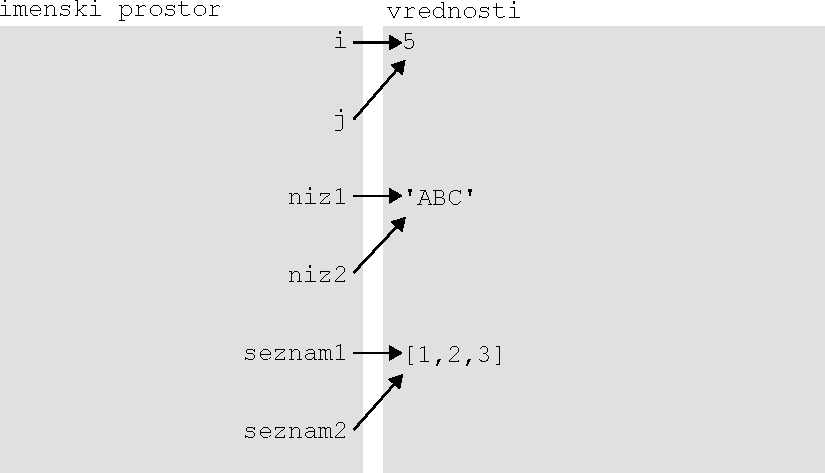
\includegraphics[width=\linewidth]{img/spremenljivost_2.pdf}
    \caption{Ob prireditvi spremenljivke drugi spremenljivki se ustvari plitva kopija spremenljivke.}
    \label{img:spremenljivost_2}
\end{figure}
Na tak način je delovanje tako s časovnega stališča (hitrost) kot tudi s prostorskega stališča (poraba pomnilnika) bolj varčno. 

\section{Kaj se zgodi ob spreminjanju vrednosti spremenljivk?}
Kaj pa se zgodi, če vrednost nove (ali pa stare) spremenljivke spremenimo? Vse skupaj zavisi od tega ali je podatek, ki ga spreminjamo spremenljiv ali ne. Spomnimo se. Spremenljiv podatek lahko spreminjamo, ko pa pokusimo spremeniti nespremenljiv podatek, se ustvari njegova kopija (globoka), ki odraža narejeno spremembo. Če npr. uporabimo operator \texttt{+=}, bo v primeru spremenljivega podatka spremenjen obstoječ podatek, v primeru nespremenljivega podatka pa bo ustvarjen nov podatek, ki bo odražal narejeno spremembo. 

Kaj pa se zgodi v primeru, da na podatek kaže več imen, kot v scenariju zgoraj. Ali se bo po izvedbi spodnje kode sprememba odražala tudi preko drugih imen podatka? Poglejmo si spodnjo kodo.
\begin{lstlisting}[language=Python]
>>> i = 1
>>> j = i
>>> j += 1
>>> niz1 = 'ABC'
>>> niz2 = niz1
>>> niz2 += 'D'
>>> seznam1 = [1,2,3]
>>> seznam2 = seznam1
>>> seznam2 += [4]
\end{lstlisting}
Zanima nas ali se po spreminjanju spremenljivk \texttt{j}, \texttt{niz2} in \texttt{seznam2} spremembe odražajo tudi na spremenljivkah \texttt{i}, \textbf{niz1} in \texttt{seznam1}. Odgovor ni enostaven da ali ne. Odgovor je namreč odvisen od spremenljivosti podatka, ki ga spreminjamo. Situacijo po spreminjanju podatka z operatorjem \texttt{+=} prikazuje slika \ref{img:spremenljivost_3}.
\begin{figure}
    \centering
    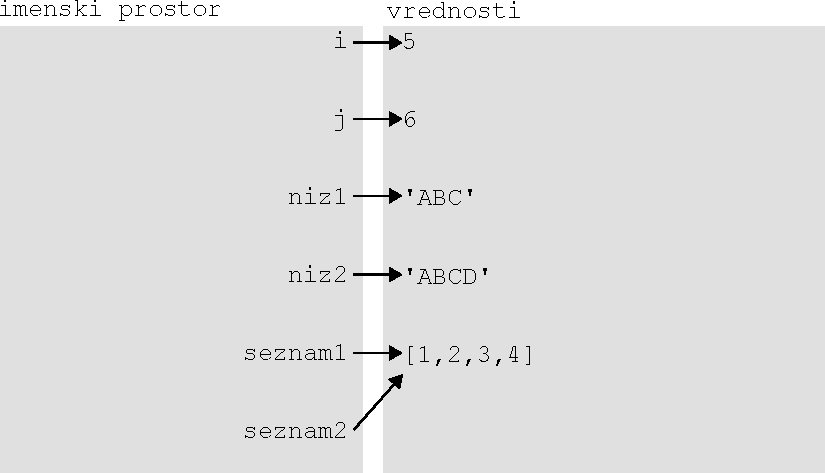
\includegraphics[width=\linewidth]{img/spremenljivost_3.pdf}
    \caption{Ob spreminjanju spremenljivih podatkov se spremenijo vse plitve kopije podatka.}
    \label{img:spremenljivost_3}
\end{figure}
V primeru, da je podatek spremenljiv, se torej sprememba odraža na vseh spremenljivkah, ki predstavljajo plitve kopije tega podatka. S tem ko v zgornjem zgledu spreminjamo spremenljivko \texttt{seznam2}, spreminjamo tudi spremenljivko \texttt{seznam1}. Po drugi strani spreminjanje spremenljivk \texttt{j} in \texttt{niz2} ustvari globoko kopijo spremenljivk \texttt{j} in \texttt{niz2}, ki odraža narejeno spremembo. Globoka kopija predstavlja nov podatek, tj. podatek ki se razlikuje od tistega, na katerega kažeta imeni \texttt{i} in \texttt{niz1}. Posledica tega je, da spreminjanje vrednosti spremenljivk \texttt{j} in \texttt{niz2} na vrednostih spremenljivk \texttt{i} in \texttt{niz1} ne vplivajo, saj pripadajo nespremenljivim podatkovnim tipom.

\section{Ali funkcije spreminjajo vrednosti svojim argumentom?}
Spomnimo se, da se ob klicu funkcije ustvari lokalni imenski prostor funkcije. V lokalnem imenskem prostoru se ob klicu spremenljivkam, ki nastopajo kot argumenti funkcije, priredijo vrednosti, s katerimi smo funkcijo poklicali. V primeru, da smo funkcijo poklicali z globalnimi spremenljivkami, se argumentom funkcije priredi plitva kopija teh spremenljivk. Vprašanje pa je ali se bodo ob spreminjanju argumentov funkcije spremembe odražale tudi izven funkcije, torej po tem, ko se bo funkcija že končala. Vprašanje lahko ponazorimo s spodnjim zgledom.

\begin{zgled}
Kakšna je vrednost spremenljivk \texttt{st1}, \texttt{niz1} in \texttt{seznam1} po izvedbi spodnje kode in kakšen bo izpis programa?
\begin{lstlisting}[language=Python,numbers=left]
def spremeni(a, b):
    a += b

i = 1
j = 2
spremeni(i,j)
print(i)

niz1 = "ABC"
niz2 = "D"
spremeni(niz1,niz2)
print(niz1)

seznam1 = [1,2,3]
seznam2 = [4,5,6]
spremeni(seznam1,seznam2)
print(seznam1)
\end{lstlisting}
\end{zgled}

\begin{resitev}
Ob klicu funkcije spremenljivki, s katerima funkcijo pokličemo, dobita plitvi kopiji z imeni \texttt{a} in \texttt{b} v lokalnem imenskem prostoru funkcije. Znotraj funkcije plitvo kopijo z imenom \texttt{a} spreminjamo. V primeru, da je spremenljivka spremenljivega podatkovnega tipa (npr. seznam) se spreminja obstoječ podatek, na katerega kaže tudi globalna spremenljivka, kar pomeni, da se bo sprememba odražala tudi izven funkcije. V primeru, da je spremenljivka nespremenljivega podatkovnega tipa, se ustvari globoka kopija podatka, ki bo odražala narejeno spremembo. Spremeni se torej zgolj spremenljivka, ki je definirana znotraj funkcije, ta sprememba pa izven funkcije ne bo vidna. 

Spremenljivki \texttt{i} in \texttt{niz1} se torej po klicu funkcije ne bosta spremenili, spremenljivka \texttt{seznam1} pa se bo spremenila. Po izvedbi programa bo izpis sledeč:

\begin{lstlisting}[language=Python]
1 # nespremenjena vrednost
ABC # nespremenjena vrednost
[1,2,3,4,5,6] # spremenjena vrednost
\end{lstlisting}

\end{resitev}

Funkcije torej lahko spreminjajo vrednosti svojim argumentom, tako da so spremembe vidne tudi izven funkcij, ampak samo v primeru, ko so podani argumenti spremenljivega podatkovnega tipa. 



\section{Terke}

Zdaj, ko vemo, kaj je to spremenljivost, lahko razložimo tudi, kaj so terke \angl{tuples}. Terka oziroma \texttt{tuple} predstavlja sekvenčen podatkovni tip, ki je nespremenljiv. Ker terke zelo spominjajo na sezname, bi jim lahko rekli tudi nespremenljivi seznami. Načeloma bi lahko pri programiranju shajali tudi brez njih (tako kot bi lahko shajali tudi brez zanke \texttt{for}), ampak njihova uporaba v veliko primerih naredi naše programe lepše in boljše (tako kot uporaba zanke \texttt{for}).

\section{Uporaba terk}

Terko definiramo z navadnimi oklepaji, tj. \texttt{(} in \texttt{)}, znotraj katerih naštejemo elemente. Terko treh elementov, bi lahko definirali na primer takole:
\begin{lstlisting}[language=Python]
>>> terka=("Janez", 1.8, 75)
\end{lstlisting}
Tudi, če bi elemente našteli brez oklepajev, bi dobili terko. Takole:
\begin{lstlisting}[language=Python]
>>> terka="Janez", 1.8, 75
>>> terka
("Janez", 1.8, 75)
>>> type(terka)
<class 'tuple'>
\end{lstlisting}
Python je ob naštevanju elementov z vejicami ugotovil, da želimo imeti terko in jo naredil. Python ima nekoliko težav, ko želimo narediti terko dolžine 1, saj si v tem primeru oklepaje razlaga kot operator, ki določa prioriteto. V primeru, da znotraj oklepajev damo zgolj eno npr. celo število, bomo torej dobili podatek, ki pripada podatkovnemu tipu \texttt{int} in ne \texttt{tuple}:
\begin{lstlisting}[language=Python]
>>> terka=(1)
>>> terka
1
>>> type(terka)
<class 'int'>
\end{lstlisting}
Ena izmed lastnosti terk je naštevanje elementov, ki jih ločimo z vejicami. Kako v primeru enega elementa povemo, da gre za naštevanje? Tako, da za njim napišemo vejico:
\texttt{tuple}:
\begin{lstlisting}[language=Python]
>>> terka=(1,)
>>> terka
(1,)
>>> type(terka)
<class 'tuple'>
\end{lstlisting}
Gre pa seveda tudi brez oklepajev:
\texttt{tuple}:
\begin{lstlisting}[language=Python]
>>> terka=1,
>>> terka
(1,)
>>> type(terka)
<class 'tuple'>
\end{lstlisting}

Kaj lahko s terkami počnemo? Podobno kot sezname lahko elemente terke indeksiramo, lahko delamo rezine, lahko preverjamo vsebovanost elementov, z zanko \texttt{for} se lahko čez elemente terke sprehajamo itd. Z njimi lahko delamo torej skoraj vse, kar smo delali s seznami. Skoraj vse? Ker so terke nespremenljive, jih seveda ne moremo spreminjati, tako kot lahko spreminjamo sezname. Poskusimo:
\begin{lstlisting}[language=Python]
>>> terka = ("Janez", 1.8, 75)
>>> terka[0] = "Marko"
TypeError: 'tuple' object does not support item assignment
\end{lstlisting}
Očitno res ne gre. Seveda ne, saj so nespremenljive. Zakaj bi terke potem sploh uporabljali? Nekaj primerov, pri katerih je uporaba terk smiselna, je podanih v nadaljevanju poglavja.

\section{Seznami terk in razpakiranje elementov terk}

Nenapisano pravilo (ki ga seveda lahko kršimo) je, da v sezname shranjujemo homogene podatke, torej podatke, ki se nanašajo npr. na isto spremenljivko. To pomeni, da vsak element seznama obravnavamo na enak način, saj se nanaša na isto količino. Terke se pogosto uporabljajo za shranjevanje heterogenih podatkov, tj. podatkov različnih tipov, ki pa pripadajo isti entiteti, kot je npr. oseba ali meritev. Če si torej želimo pri določeni entiteti zabeležiti več podatkov, lahko uporabimo seznam terk. Na primer, če imamo vzorec oseb, pri čemer za vsako osebo beležimo ime, višino in telesno maso, potem lahko uporabimo seznam terk, pri čemer vsaka izmed terk vsebuje ime, višino in telesno maso dotične osebe. Primer takega seznama bi bil
\begin{lstlisting}[language=Python]
meritve = [("Janez", 1.8, 75),
           ("Ana", 1.65, 60), 
           ("Nika", 1.66, 55)]
\end{lstlisting}
Elementi seznama so torej homogeni, kar pomeni, da bomo vsakega obravnavali enako. Elementi seznama so namreč terke, ki imajo vsakič enako obliko. Na 0-tem indeksu je shranjeno ime osebe, na indeksu 1 višina v metrih in na indeksu 2 telesna masa osebe v kilogramih. Elementi posamezne terke pa očitno pripadajo različnim spremenljivkam.

Tak način predstavitve podatkov bomo srečali velikokrat. Kako pa lahko tako shranjene podatke uporabimo pri nadaljnji analizi. Na primer pri izračunu in izpisu indeksa telesnih mas posamezne osebe v seznamu. Tako, da se čez seznam sprehodimo z zanko \texttt{for} in v vsaki iteraciji zanke tekočo terko \emph{razpakiramo} in tako pridemo do konkretnih vrednosti. To lahko naredimo na sledeč način: 
\begin{lstlisting}[language=Python]
for meritev in meritve:
    ime = meritev[0]
    visina = meritev[1]
    masa = meritev[2]
    itm = masa/visina**2
    print("ITM osebe", ime, "je", itm)
\end{lstlisting}
Do posameznih elementov terke smo torej prišli z njihovim indeksiranjem. Terke pa lahko razpakiramo veliko hitreje, in sicer tako, da terko priredimo drugi terki, ki vsebuje imena spremenljivk, v katere želimo vrednosti shraniti oziroma razpakirati. Takole:
\begin{lstlisting}[language=Python]
(spremenljivka1, spremenljivka2,...) = terka
\end{lstlisting}
Paziti moramo le na to, da terka na levi strani vsebuje enako število elementov kot terka na desni strani prireditvenega stavka. Kaj smo v zgornjem stavku pravzaprav naredili? Naredili smo terko spremenljivk, ki smo ji priredili terko na desni strani. Ker terki spremenljivk nismo dali nobenega imena, je v imenski prostor nismo shranili in zato tudi ni shranjena nikjer v pomnilniku. So pa v pomnilniku ostale spremenljivke, v katere smo razpakirali terko na desni. Kot smo videli že zgoraj pa lahko oklepaje pri definiciji tudi izpustimo. Torej lahko napišemo tudi nekaj takega
\begin{lstlisting}[language=Python]
spremenljivka1, spremenljivka2,... = terka
\end{lstlisting}
Mimogrede, tako razpakiranje elementov bi delovalo tudi, če bi imeli na desni strani prireditvenega stavka seznam.

Tak način razpakiranja elementov lahko uporabimo v našem zgledu z računanjem indeksa telesnih mas, s čimer se koda občutna skrajša:
\begin{lstlisting}[language=Python]
for meritev in meritve:
    ime, visina, masa = meritev
    itm = masa/visina**2
    print("ITM osebe", ime, "je", itm)
\end{lstlisting}
Kodo lahko še dodatno skrajšamo, če razpakiranje naredimo kar v glavi zanke \texttt{for}:
\begin{lstlisting}[language=Python]
for ime, visina, masa in meritve:
    itm = masa/visina**2
    print("ITM osebe", ime, "je", itm)
\end{lstlisting}

\section{Pakiranje seznamov v sezname terk}
Seznami terk, kot smo jih srečali zgoraj, torej predstavljajo lep način zapisovanja podatkov, ko želimo pri posamezni entiteti imeti več podatkov. Dejstvo pa je, da velikokrat podatkov ne dobimo v taki obliki, ampak dobimo za vsako količino svoj seznam. Pri tem so seznami med seboj poravnani, kar pomeni, da istoležni elementi v vseh seznamih pripadajo isti entiteti. Elementi na indeksu 0 torej pripadajo entiteti 0, elementi na indeksu 1 entiteti 1 itd. V primeru imen, višin in mas, bi torej imeli tri sezname v obliki 
\begin{lstlisting}[language=Python]
imena = ["Janez", "Ana", "Nika"]
visine = [1.8, 1.65, 1.66]
mase = [75, 60, 55]
\end{lstlisting}
Elementi vseh treh seznamov torej na indeksu 0 pripadajo Janezu, na indeksu 1 Ani in na indeksu 2 Niki. Kaj imajo ti seznami skupnega? Indekse! Čez take podatke bi se torej lahko sprehodili tako, da se sprehajamo po indeksih in ne direktno po elementih. Naredimo torej sprehod z znako \texttt{for} od indeksa 0 do dolžine seznama - 1. Dolžine katerega seznama? Ni važno, saj so vsi enko dolgi (oziroma vsaj smiselno bi bilo, da so). To bi lahko naredili takole:  
\begin{lstlisting}[language=Python]
for i in range(len(imena)):
    ime = imena[i]
    visina = visine[i]
    masa = mase[i]
    itm = masa/visina**2
    print("ITM osebe", ime, "je", itm)
\end{lstlisting}
Kako pa bi lahko iz treh seznamov naredili seznam terk, s katerim smo delali zgoraj. Izkaže se, da se s takim problemom srečamo relativno pogosto, zato nam Python za \emph{zapakiranje} več seznamov v seznam terk ponuja vgrajeno funkcijo \texttt{zip}. Funkcija \texttt{zip} iz zgornjih treh seznamov naredi točno to, kar bi si želeli: 
\begin{lstlisting}[language=Python]
>>> meritve = zip(imena, visine, mase)
>>> meritve
<zip object at 0x0000019A2A865D48>
\end{lstlisting}
Tale izpis je malo čuden, ampak ni z njim nič narobe. Funkcija \texttt{zip} je t.i. \emph{iterator}, ki dejanski element seznama terk vrne, šele ko ga potrebujemo, oziroma posamezne elemente seznama vrača sproti. Če bi želeli imeti lepši izpis, bi lahko do njega prišli tako, da rezultat funkcije \texttt{zip} eksplicitno pretvorimo v seznam s funkcijo \texttt{list}:
\begin{lstlisting}[language=Python]
>>> meritve = list(zip(imena, visine, mase))
>>> meritve
[('Janez', 1.8, 75), ('Ana', 1.65, 60), ('Nika', 1.66, 55)]
\end{lstlisting}
Sprehod čez sezname lahko torej naredimo na podoben način kot v prejšnjem poglavju, le da prej sezname zapakiramo v seznam terk:
\begin{lstlisting}[language=Python]
for ime, visina, masa in zip(imena, visine, mase):
    itm = masa/visina**2
    print("ITM osebe", ime, "je", itm)
\end{lstlisting}

\section{Zahteva po nespremenljivosti}
V določenih primerih Python zahteva uporabo nespremenljivih podatkovnih tipov. Nespremenljive podatkovne tipe moramo uporabiti, kadar želimo podatke shranjevati v množico (\texttt{set}) in kadar želimo nek podatek uporabiti kot ključ (\texttt{key}) slovarja (\texttt{dict}). Če želimo v takem primeru uporabiti več elementov, moramo namesto po seznamu poseči po terki. V teh primerih je torej uporaba terk obvezna. Več o množicah in slovarjih bomo izvedeli prav kmalu.

Drug primer, v katerem bi nespremenljivost bila zaželena (ne pa obvezna), je, ko ne želimo, da funkcija spremeni vrednosti podanega argumenta. Kot smo videli lahko funkcije spreminjajo vrednosti svojih argumentov, tako da bodo spremembe vidne tudi izven funkcij. Če bi radi zagotovilo, da se podan argument izven funkcije zagotovo ne bo spremenil, namesto spremenljivega seznama enostavno uporabimo nespremenljivo terko. V tem kontekstu si poglejmo spodnji zgled.

\begin{zgled}
Kakšna je vrednost spremenljivk \texttt{seznam1} in \texttt{terka1}  po izvedbi spodnje kode in kakšen bo izpis programa?
\begin{lstlisting}[language=Python,numbers=left]
def spremeni(a, b):
    a += b

seznam1 = [1,2,3]
seznam2 = [4,5,6]
spremeni(seznam1,seznam2)
print(seznam1)

terka1 = (1,2,3)
terka2 = (4,5,6)
spremeni(terka1,terka2)
print(terka1)
\end{lstlisting}
\end{zgled}

\begin{resitev}
Kot smo videli že prej, se sprememba, ki smo jo nad plitvo kopijo spremenljivke \texttt{seznam1} naredili znotraj funkcije, odraža tudi izven funkcije, saj je seznam spremenljiv podatkovni tip. Ko torej spreminjamo njegovo plitvo kopijo, s tem spreminjamo vse spremenljivke, ki nanj kažejo. 

Kaj pa se zgodi, ko funkcijo pokličemo s terko. Najprej se ustvari plitva kopija terke v lokalnem imenskem prostoru funkcije (spremenljivka \texttt{a}). Ker je terka nespremenljiv podatkovni tip, je ne moremo spreminjati. Ob njenem spreminjanju se zato ustvari globoka kopija, torej nov podatek v pomnilniku, ki odraža narejeno spremembo. Na ta podatek pa kaže zgolj lokalna spremenljivka \texttt{a}. Ko se funkcija zaključi, njen lokalni imenski prostor skupaj z lokalno spremenljivko \texttt{a} izgine (tako kot tudi spremenjena terka -- globoka kopija terke, s katero smo funkcijo poklicali). V sled temu sprememba, ki smo jo naredili znotraj funkcije, izven funkcije ni vidna.

Po izvedbi funkcije \texttt{spremeni} ima spremenljivka \texttt{seznam1} spremenjeno vrednost (\texttt{[1,2,3,4,5,6]}), spremenljivka \texttt{terka1} pa ostane taka, kot je bila pred klicem funkcije (\texttt{(1,2,3)}). Izpis programa je torej
\begin{lstlisting}[language=Python]
[1,2,3,4,5,6] # spremenjena vrednost
(1,2,3) # nespremenjena vrednost
\end{lstlisting}

\end{resitev}

Funkcijam, ki kot argumente sprejemajo spremenljive podatkovne tipe, spremenjenih vhodnih argumentov ni potrebno vračati, saj se bodo spremembe odražale tudi izven funkcije. Funkcije, ki kot argumente sprejemajo nespremenljive podatkovne tipe, morajo spremenjene vhodne argumente eksplicitno vrniti, saj so spremenjene vrednosti sicer za vedno izgubljene. Oba načina si poglejmo v spodnjih zgledih.

Najprej si poglejmo kako se lotiti pisanja in uporabe funkcije, ki sprejema nespremenljive podatke.
\begin{zgled}
Napiši funkcijo \texttt{dodaj\_AT\_niz}, ki sprejme dve nukleotidini zaporedji zapisani kot niza in v prvo zaporedje doda vse ponovitve baz \texttt{A} in \texttt{T} v enakem zaporedju kot nastopajo v drugem nizu. Funkcijo uporabi na zaporedjih \texttt{'ATCG'} in \texttt{'AATGGAATGG'}, tako da bo prvo zaporedje po njeni izvedbi spremenjeno.
\end{zgled}

\begin{resitev}
Funkcija sprejema in spreminja podatke tipa \texttt{str}, ki je nespremenljiv podatkovni tip. Če bomo vhodne argumente spreminjali znotraj funkcije, se te spremembe izven funkcije ne bodo odražale, kar pomeni, da mora funkcija vračati spremenjen niz. Napišimo jo.
\begin{lstlisting}[language=Python]
def dodaj_AT_niz(zaporedje1, zaporedje2):
    for baza in zaporedje2:
        if baza in 'AT':
            zaporedje1 += baza
    return zaporedje1
\end{lstlisting}
Na koncu torej vrnemo spremenjeno zaporedje1. Kljub temu, da smo znotraj funkcije to spremenljivko spreminjali, spremembe izven funkcije ne bodo vidne.

Klic funkcije moramo izvesti na tak način, da bo spremenila vrednost prve spremenljive, s katero funkcijo kličemo. Kako to doseči? Enostavno tako, da rezultat funkcije priredimo tej spremenljivki. Takole:
\begin{lstlisting}[language=Python]
>>> zaporedje1 = 'ATCG'
>>> zaporedje2 = 'AATGGAATGG'
>>> zaporedje1 = dodaj_AT_niz(zaporedje1, zaporedje2)
\end{lstlisting}
Na tak način smo vrednost spremenljivke \texttt{zaporedje1} spremenili.
\end{resitev}

Poglejmo si še kakšne so razlike pri delu s spremenljivimi podatki.
\begin{zgled}
Napiši funkcijo \texttt{dodaj\_AT\_seznam}, ki sprejme dve nukleotidini zaporedji zapisani kot seznama enoznakovnih nizov (baz) in v prvo zaporedje doda vse ponovitve baz \texttt{A} in \texttt{T} v enakem zaporedju kot nastopajo v drugem nizu. Funkcijo uporabi na zaporedjih \texttt{['A','T','C','G']} in \texttt{'A','A','T','G','G','A','A','T','G','G'}, tako da bo prvo zaporedje po njeni izvedbi spremenjeno.
\end{zgled}
\begin{resitev}
Navodilo naloge je praktično enako kot prej, le da tokrat namesto nespremenljivih podatkovnih tipov uporabljamo spremenljive. To pomeni, da ni potrebe po tem, da funkcija vrača spremenjen rezultat, saj se bodo spremembe odražale že preko podanega argumenta. Koda je torej sledeča:
\begin{lstlisting}[language=Python]
def dodaj_AT_seznam(zaporedje1, zaporedje2):
    for baza in zaporedje2:
        if baza in 'AT':
            zaporedje1.append(baza)
\end{lstlisting}
Tokrat funkcija ne vrača ničesar uporabnega, zato njenega rezultata nima smisla ničemur prirejati. Vse kar potrebujemo je klic funkcije z ustreznimi argumenti:
\begin{lstlisting}[language=Python]
>>> zaporedje1 = ['A','T','C','G']
>>> zaporedje2 = ['A','A','T','G','G','A','A','T','G','G']
>>> dodaj_AT_seznam(zaporedje1, zaporedje2) 
\end{lstlisting}
Prepričajmo se, če je vrednost spremenljivke \texttt{zaporedje1} res spremenjena:
\begin{lstlisting}[language=Python]
>>> zaporedje1
['A', 'T', 'C', 'G', 'A', 'A', 'T', 'A', 'A', 'T']
\end{lstlisting}
\end{resitev}
\chapter{Slovarji}

\section{Zakaj slovarji?}

Zdaj smo se že pobliže spoznali z različnimi sekvenčnimi podatkovnimi tipi, med katere smo uvrstili nize, sezname in terke. V spremenljivke, ki so pripadale tem tipom, smo lahko shranili več podatkov, pri čemer je bil podatek vedno povezan z določenim indeksom. Če se osredotočimo na sezname (kar bomo povedali velja sicer tudi za nize in terke), lahko rečemo, da so podatki v njih na nek način urejeni, ko smo v sezname dodajali nove podatke, smo te ponavadi dodajali na konec seznama, iskanje pa je potekalo tako, da smo se morali z zanko \texttt{for} sprehoditi čez celoten seznam in iskati dokler elementa nismo našli. Sezname smo lahko tudi sortirali po nekem ključu (recimo glede na relacijo <), pri čemer je bil rezultat sortiranja tak, da je manjši ključ imel manjšo vrednost glede na uporabljeno relacijo. 

V določenih primerih pa je bolj priročno, če lahko do vrednosti v spremenljivki dostopamo še preko česa drugega kot njenega indeksa. Pomislimo npr. na telefonski imenik števil, kjer lahko do telefonske številke neke osebe, dostopamo preko imena te osebe. Rekli bi lahko, da je ime osebe \emph{ključ} preko katerega dostopamo do telefonske številke oziroma \emph{vrednosti}. Na podoben način iščemo gesla v Slovarju slovenskega knjižnjega jezika (ali pač kakšnem drugem slovarju), kjer kot ključ nastopa iskana beseda oziroma geslo, kot vrednost pa razlaga iskane besede. Za razlago določene besede nam torej ni potrebno preiskati celotnega slovarja, ampak njeno razlago poiščemo preko gesla, ki ga je v slovarju načeloma enostavno najti.

Takim imenikom in slovarjem ustreza podatkovna struktura \texttt{dict} \angl{dictionary} oziroma po slovensko kar \emph{slovar}. V primeru slovarjev posamezna \emph{vrednost} \angl{value} ni vezana na določen indeks, ampak je povezana na  \emph{ključ} \angl{key}. Elemente slovarja torej vedno podajamo kot pare \emph{ključ:vrednost}. Kakšna je prednost takega načina shranjevanja podatkov? Uporabna je takrat, ko ključe, po katerih shranjujemo in kasneje iščemo vrednosti, poznamo. V tem primeru je iskanje zelo hitro, saj nam ni potrebo preiskati celotnega slovarja, ampak slovarju zgolj podamo ključ in do vrednosti pridemo takoj. Operacija iskanja je torej zelo hitra v primerjavi s seznami ali terkami.

\section{Kako uporabljamo slovarje?}

Slovarje zapisujemo z zavitimi oklepaji, torej \texttt{\{} in \texttt{\}}, pri čemer elemente naštejemo kot pare ključ in vrednost ločene z dvopičjem (\texttt{:}). Prazen slovar bi naredili takole
\begin{lstlisting}[language=Python]
>>> prazen_slovar = {}
\end{lstlisting}
Slovar, ki vsebuje enostaven telefonski imenik bi lahko zapisali kot
\begin{lstlisting}[language=Python]
>>> imenik = {"Janez":"083455544", 
            "Ana":"084566732", 
            "Nika":"099563123"}
\end{lstlisting}
V tem primeru so ključi slovarja nizi, ki predstavljajo imena oseb, preko katerih lahko pridemo vrednosti, ki v tem primeru predstavljajo telefonske številke zapisane kot nizi. 

Mimogrede, slovar je spremenljiv podatkovni tip, kot smo zapisali že v tabeli \ref{tab:spremenljivost}.

\section{Iskanje vrednosti}
Telefonsko številko osebe lahko torej najdemo tako, da podamo njeno ime, kar je smiselno, saj imena svojih prijateljev ponavadi poznamo na pamet, njihovih telefonskih številk pa ne. Telefonsko številko od Janeza lahko npr. dobimo tako, da slovar indeksiramo po ključu \texttt{"Janez"}:
\begin{lstlisting}[language=Python]
>>> imenik["Janez"]
083455544
\end{lstlisting}
Indeksiranje se torej v primeru slovarjev namesto po indeksih izvaja po ključih. Kaj pa če bi želeli poiskati telefonsko številko od Dejana. Potem bi slovar indeksirali po ključu \texttt{"Dejan"}, kar pa nam v konkretnem primeru vrne napako:
\begin{lstlisting}[language=Python]
>>> imenik["Dejan"]
Traceback (most recent call last):
  File "<pyshell#1>", line 1, in <module>
    imenik["Dejan"]
KeyError: 'Dejan'
\end{lstlisting}
Problem je v tem, da ključa \texttt{"Dejan"} v našem slovarju (še) ni, zato preko njega slovarja ne moremo indeksirati (tako kot nismo mogli indeksirati seznam z indeksom, ki ga v seznamu ni bilo). Obstoj ključa v slovarju lahko preverimo z operatorjem \texttt{in}:
\begin{lstlisting}[language=Python]
>>> "Dejan" in imenik
False
>>> "Nika" in imenik
True
\end{lstlisting}
Preden do določenega ključa v slovarju dostopamo je torej smiselno, da preverimo, če ključ v slovarju sploh obstaja.
\begin{zgled}
Napiši funkcijo \texttt{poisci}, ki kot argument sprejme imenik in ime osebe. Če imena ni v imeniku naj funkcija vrne vrednost \texttt{False}, sicer pa njeno telefonsko številko.
\end{zgled}
\begin{resitev} Rešitev mora pred indeksiranjem po podanem ključu, preveriti, če ključ v slovarju obstaja. V nasprotnem primeru vrne vrednost \texttt{False}. 
\begin{lstlisting}[language=Python]
def poisci(imenik, ime):
    if ime in imenik:
        return imenik[ime]
    else:
        return False
\end{lstlisting}
\end{resitev}

\section{Dodajanje in spreminjanje vrednosti}

Indeksiranje po ključih, ki jih v slovarju ni, pa je v določenih primerih dovoljeno, in sicer takrat, ko želimo v slovar dodati nov par ključ, vrednost. Dodajanje novega elementa lahko torej izvedemo tako, da slovar indeksiramo po novem (neobstoječem) ključu in takemu indeksrianju priredimo vrednost, ki jo želimo s tem ključem povezati. Če bi npr. želeli v slovar dodati Dejana in z njim povezati neko telefonsko številko, npr. 089543678, bi to naredili takole:
\begin{lstlisting}[language=Python]
>>> imenik["Dejan"] = "089543678"
\end{lstlisting}
V tem primeru napake nismo dobili, v slovarju pa se je ponavil nov par ključ, vrednost.
\begin{lstlisting}[language=Python]
>>> imenik
{'Janez': '083455544', 'Ana': '084566732', 
'Nika': '099563123', 'Dejan': '089543678'}
\end{lstlisting}

Kaj pa se zgodi, če poskusimo v slovar dodati še enega Dejana? Ker v slovarju do vrednosti dostopamo preko ključev, morajo biti ključi enolični, kar pomeni, da se posamezen ključ lahko v slovarju pojavi največ enkrat. Če torej naredimo prireditev vrednosti preko ključa, ki v slovarju že obstaja, bomo s tem izvedli spreminjanje vrednosti, ki je povezana s tem ključem. Prireditev
\begin{lstlisting}[language=Python]
>>> imenik["Dejan"] = "000000000"
\end{lstlisting}
bo torej spremenila telefonsko številko Dejana na 000000000.
\begin{lstlisting}[language=Python]
>>> imenik
{'Janez': '083455544', 'Ana': '084566732', 
'Nika': '099563123', 'Dejan': '000000000'}
\end{lstlisting}

Če bi se želeli torej omejiti samo na dodajanje elementov, bi lahko prej preverili, če ključ preko katerega dodajamo v slovarju že obstaja in dodajanje izvedli le, če takega ključa še ni.
\begin{zgled}
Napiši funkcijo \texttt{dodaj}, ki kot argumente prejme imenik, ime osebe in telefonsko številko osebe. Osebo in njeno telefonsko številko naj v slovar doda samo v primeru, če te osebe še ni v slovarju. Sicer naj izpiše, da ta oseba že obstaja.
\end{zgled}
\begin{resitev}
V funkciji bomo tokrat izvedli prirejanje vrednosti, samo če podanega ključa še ni v slovarju. Poraja pa se dodatno vprašanje. Ali mora funkcija spremenjen slovar vračati? Odgovor je ne, saj je slovar spremenljiv podatkovni tip in sprememembe slovarja, ki jih bomo v funkciji naredili in ki ga je funkcija prejela kot argument, se bodo odražale tudi izven funkcije.
\begin{lstlisting}[language=Python]
def dodaj(imenik, ime, stevilka):
    if ime not in imenik:
        imenik[ime] = stevilka
    else:
        print("Ta oseba ze obstaja")
\end{lstlisting}
\end{resitev}

Če bi se želeli samo na spreminjanje elementov, bi morali spremeniti pogoj v stavku \texttt{if}, tako da številko prirejamo samo v primeru, če je ključ v slovarju že vsebovan.
\begin{zgled}
Napiši funkcijo \texttt{spremeni}, ki kot argumente prejme imenik, ime osebe in telefonsko številko osebe. Telefonsko številko naj spremeni samo v primeru, če je oseba v imeniku že vsebovana. Sicer naj izpiše, da te osebe v imeniku ni.
\end{zgled}
\begin{resitev}
Tokrat bomo v funkciji izvedli prirejanje vrednosti samo v primeru, če podan ključ v slovarju je. V nasprtonem primeru ne bi izvajali spreminjanja vrednosti za ključem, ampak bi izvajali dodajanje novega para ključ, vrednost.
\begin{lstlisting}[language=Python]
def spremeni(imenik, ime, stevilka):
    if ime in imenik:
        imenik[ime] = stevilka
    else:
        print("Te osebe ni v imeniku")
\end{lstlisting}
\end{resitev}

V določenih primerih, npr. pri štetju pojavitev nečesa, moramo v slovar dodati nov ključ, če tega ključa v slovarju še ni, ali spreminjati nanj vezano vrednost, če ta ključ v slovarju že obstaja. Poglejmo si sledeč primer:

\begin{zgled}
Napiši funkcijo \texttt{prestej\_baze}, ki kot argument prejme nukleotidno zaporedje baz zapisano kot niz. Funkcija naj vrne slovar, ki za posamezno bazo vsebuje število ponovitev.
\end{zgled}
\begin{resitev}
Za razliko od prej bo funkcija slovar vračala, saj ji ga kot argument nismo podali. V programu bi lahko predpostavljali, da delamo samo z bazami A, T, C in G. Tako bi si na začetku naredili slovar, v katerem kot ključi nastopajo oznake baz, nanje pa so vezane vrednosti 0. Takole:
\begin{lstlisting}[language=Python]
baze = {'A':0, 'T':0, 'C':0, 'G':0}
\end{lstlisting}
Slabost takega pristopa je ta, da smo se omejili samo na ključe A, T, C in G. Kaj pa če kot vhod dobimo RNA zaporedje? Ali pa če se v zaporedju pojavi še kakšna oznaka, ki je nismo predvideli?

Boljši pristop bi bil, da na začetku naredimo prazen slovar in ko v nizu najdemo bazo, ki je v slovarju še ni, nanjo vežemo vrednost 1 (če smo jo našli v nizu prvič, potem to pomeni, da smo jo našli enkrat). V primeru, da v nizu najdemo bazo, ki v slovarju že obstaja, število njenih pojavitev povečamo za 1. 
\begin{lstlisting}[language=Python]
def prestej_baze(zaporedje):
    baze = {} # prazen slovar
    for baza in zaporedje:
        if baza not in baze: # baza v slovarju? 
            baze[baza] = 1 # ne
        else:
            baze[baza] += 1 # da
    return baze
\end{lstlisting}

\end{resitev}


\section{Brisanje vrednosti}

V določenih primerih želimo elemente iz slovarjev tudi brisati. To lahko naredimo z besedico \texttt{del}, ki smo jo srečali že pri brisanju elementov iz seznama. Podobno kot pri seznamih tudi iz slovarjrv brišemo z indeksiranjem vrednosti, ki jo želimo izbrisati:
\begin{lstlisting}[language=Python]
del slovar[kljuc]
\end{lstlisting}
Tudi tokrat je smiselno, da pred brisanjem preverimo, če podan ključ v slovarju obstaja (brisanje po neobstoječem ključu bo spet vrnilo napako).

\begin{zgled}
Napiši funkcijo \texttt{izbrisi}, ki kot argumente prejme imenik in ime osebe, ki jo želimo iz imenika izbrisati. Brisanje naj se izvede samo v primeru, ko oseba v imeniku obstaja. Sicer naj funkcija izpiše, da te osebe v imeniku ni.
\end{zgled}
\begin{resitev}
Spet bomo najprej preverili obstoj ključa, nato pa izvedli brisanje.
\begin{lstlisting}[language=Python]
def izbrisi(imenik, ime):
    if ime in imenik:
        del imenik[ime]
    else:
        print("Te osebe ni v imeniku")
\end{lstlisting}
\end{resitev}

\section{Ključi in vrednosti}

Posamezen ključe se lahko v slovarju pojavi največ enkrat. Ključi so torej enolični identifikatorji, preko katerih pridemo do posamezne vrednost. Za ključe pa velja tudi to, da morajo biti nespremenljivi. Zakaj? Vrednost, ki je vezana na posamezen ključ, se zapiše na lokacijo v pomnilniku, ki je določena s preslikavo ključa \angl{hash function}. Če ključ spreminjamo, se bo spremenila tudi vrednost preslikave. Za pravilno delovanje torej ključev ne smemo spreminjati (ko so enkrat shranjeni v slovarju). Zato je smiselno, da so ključi nespremenljivi podatki. Za vrednosti ni nobene omejitve -- uporabimo lahko poljuben podatkovni tip vključno z drugim, vgnezdenim, slovarjem.

Sicer lahko do vseh ključev v slovarju pridemo z uporabo metode \texttt{keys}, do vseh vrednosti z uporabo metode \texttt{values}, do vseh parov pa z uporabo metode \texttt{items}. 
\begin{lstlisting}[language=Python]
>>> imenik.keys()
dict_keys(['Janez', 'Ana', 'Nika', 'Dejan'])
>>> imenik.values()
dict_values(['083455544', '084566732', '099563123', 
'089543678'])
>>> imenik.items()
dict_items([('Janez', '083455544'), ('Ana', '084566732'), 
('Nika', '099563123'), ('Dejan', '089543678')])
\end{lstlisting}
Metode vračajo nekaj kar je zelo podobno seznamom. Pri metodi \texttt{keys} tako dobimo seznam ključev, pri metodi \texttt{values} seznam vrednosti, pri metodi \texttt{items} pa seznam terk. Nad rezultatom, ki ga posamezna metoda vrne, se lahko sprehajamo z zanko \texttt{for}. Zanko \texttt{for} pa lahko izvedemo tudi direktno nad slovarjem, pri čemer se bomo tako sprehajali čez ključe slovarja:
\begin{lstlisting}[language=Python]
>>> for k in imenik()
        print(k)
Janez
Ana
Nika
Dejan
\end{lstlisting}
Preko ključev seveda lahko dostopamo tudi do vrednosti. 
\begin{zgled}
Napiši funkcijo \texttt{izpisi\_imenik}, ki kot argument prejme imenik. Funkcija naj izpiše vsebino imenika, tako da se vsak vnos nahaja v svoji vrstici, ime in telefonska številka pa naj bosta ločena z dvopičjem.
\end{zgled}
\begin{resitev}
V zanki \texttt{for} se lahko sprehajamo direktno čez slovar (sprehod čez ključe), čez ključe preko metode \texttt{keys} ali pa čez pare preko metode \texttt{items}. Uporabimo tokrat zadnjo možnost.
\begin{lstlisting}[language=Python]
def izpisi_imenik(imenik):
    for ime, stevilka in slovar.items():
        print(ime, ":", stevilka)   
\end{lstlisting}
\end{resitev}

Podoben sprehod bi lahko naredili tudi kadar npr. iščemo največjo vrednost v slovarju. 
\begin{zgled}
Napiši funkcijo \texttt{naj\_baza}, ki kot argument sprejme zaporedje baz, vrne pa ime baze, ki se v zaporedju pojavi največkrat. Pri tem si pomagaj s funkcijo \texttt{prestej\_baze}. 
\end{zgled}
\begin{resitev}
Najprej bomo poklicali funkcijo \texttt{prestej\_baze}, ki bo iz niza naredila slovar pojavitev baz. V naslednjem koraku moramo najti bazo, ki ima največ pojavitev. To bomo naredili na podoben način, kot smo izvedli iskanje največjega (ali najmanjšega) elementa v seznamu -- s sprehodom z uporabo zanke \texttt{for}.

\begin{lstlisting}[language=Python]
def naj_baza(zaporedje):
    baze = prestej_baze(zaporedje)
    
    naj_B = "" # naj baza
    M = 0 # stevilo pojavitev
    for baza in baze:
        pojavitev = baze[baza]
        if pojavitev > M:
            naj_B = baza
            M = pojavitev
    return naj_B 
\end{lstlisting}


\end{resitev}
\chapter{Množice}

\section{In še množice}

Zadnji izmed vgrajenih podatkovnih tipov, ki si ga moramo pogledati, so množice. Množice za predstavitev podatkov uporabljamo takrat, ko želimo, da posamezen podatek obravnavamo največ enkrat. Ker nam Python poleg tega nad množicami omogoča izvedbo osnovnih operacij, kot so unija, presek in razlika, množice zelo spominjajo na matematične množice. 

\section{Uporaba množic}

Množice podobno kot slovarje zapisujemo v zavite oklepaje, znotraj katerih naštejemo elemente. Množico elementov 1, 2 in 3, bi torej naredili takole:
\begin{lstlisting}[language=Python]
>>> mnozica = {1,2,3}
>>> mnozica
{1, 2, 3}
>>> type(mnozica)
<class 'set'>
\end{lstlisting}
Kljub temu, da množice uporabljajo podoben zapis kot slovarji, ju Python med seboj brez problemov loči, saj slovarji za razliko od množic vsebujejo pare ključ: vrednost. Do težave pride le takrat, ko je množica oziroma slovar prazen. Do praznega slovarja pridemo tako, da podamo zavite oklepaje brez elementov:
\begin{lstlisting}[language=Python]
>>> slovar = {}
>>> slovar
{}
>>> type(slovar)
<class 'dict'>
\end{lstlisting}
Do prazne množice pridemo z uporabo funkcije \texttt{set}, ki jo pokličemo brez argumentov:
\begin{lstlisting}[language=Python]
>>> mnozica = set()
>>> mnozica
set()
>>> type(mnozica)
<class 'set'>
\end{lstlisting}

\section{Omejitve pri uporabi množic}

Elementi množic imajo zelo podobne omejitve kot ključi slovarji, za katere prav tako velja, da lahko posamezno vrednost vsebujejo največ enkrat. Prav tako kot za ključe slovarjev tudi za množice velja, da lahko vsebujejo le nespremenljive podatkovne tipe. 

Množice predstavljajo neurejeno strukturo, kar pomeni, da vrstni red elementov množice ni pomemben in tudi ni določen. Elementi torej niso vezani na indekse, zato množic ne moremo indeksirati in nad njimi delati rezine:
\begin{lstlisting}[language=Python]
>>> mnozica = {1,2,3}
>>> mnozica[0]
TypeError: 'set' object is not subscriptable
\end{lstlisting}
Prav tako nad množicami ne moremo izvajati aritmetičnih operacij, kot smo jih npr. lahko izvajali nad nizi:
\begin{lstlisting}[language=Python]
>>> {1,2,3}*3
TypeError: unsupported operand type(s) for *: 'set' and 'int'
>>> {1,2,3} + {4,5,6}
TypeError: unsupported operand type(s) for +: 'set' and 'set'
\end{lstlisting}

\section{Osnovne operacije nad množicami}

Kaj pa pravzaprav potem z množicami sploh lahko počnemo. Ko množico enkrat imamo se lahko čez njo sprehajamo z zanko \texttt{for}:
\begin{lstlisting}[language=Python]
>>> mnozica = {1,2,3}
>>> for element in mnozica:
	print(element)
1
2
3
\end{lstlisting} 
Poleg tega lahko preverjamo ali množica določen element vsebuje (ali ne) z operatorjema vsebovanosti:
\begin{lstlisting}[language=Python]
>>> mnozica = {1,2,3}
>>> 1 in mnozica
True
>>> 2 not in mnozica
False
>>> 4 in mnozica
False
\end{lstlisting}

Številu elementov v množici pravimo tudi moč množice, do katere pridemo enostavno s klicem vgrajene funkcije \texttt{len}
\begin{lstlisting}[language=Python]
>>> len({1,2,3})
3
\end{lstlisting}

\begin{zgled}
Napiši funkcijo \texttt{razlicni}, ki kot argument sprejme niz, kot rezultat pa vrne število različnih znakov, ki v nizu nastopajo
\end{zgled}
\begin{resitev}
Najprej bomo niz pretvorili v množico s funkcijo \texttt{set}. Ker množica posamezen element vsebuje največ enkrat, se bomo s tem znebili vseh potencialnih ponovitev znakov. Potem samo še izračunamo in vrnemo moč množice.
\begin{lstlisting}[language=Python,numbers=left]
def razlicni(niz):
    mnozica = set(niz) # odstranitev duplikatov
    return len(mnozica) # moc mnozice
\end{lstlisting}
\end{resitev}

Tudi primerjalni operatorji so zdaj prilagojeni matematični interpretaciji množic. Ali je prva množica podmnožica druge, lahko npr. ugotovimo z operatorjem \texttt{<=}:
\begin{lstlisting}[language=Python]
>>> {1,2,3} <= {1,2,3,4}
True
\end{lstlisting}

\section{Presek, unija in razlika}

Primeri najbolj tipičnih operacij, ki jih prikazujejo diagrami na sliki \ref{img:mnozice}, so seveda presek (\texttt{A \& B}), unija (\texttt{A | B}) in razlika (\texttt{A - B}).
\begin{figure}
    \centering
    \begin{tabular}{cc}
    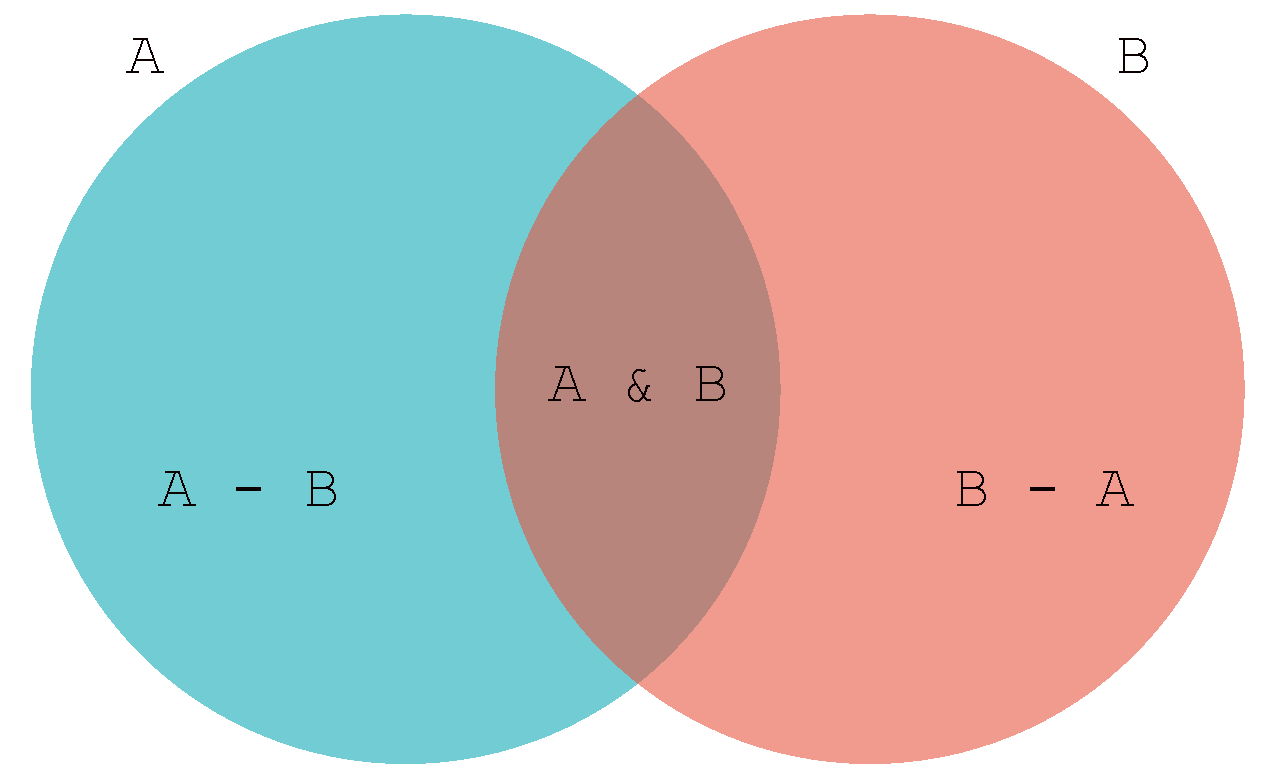
\includegraphics[width=0.45\linewidth]{img/mnozice1.pdf} & 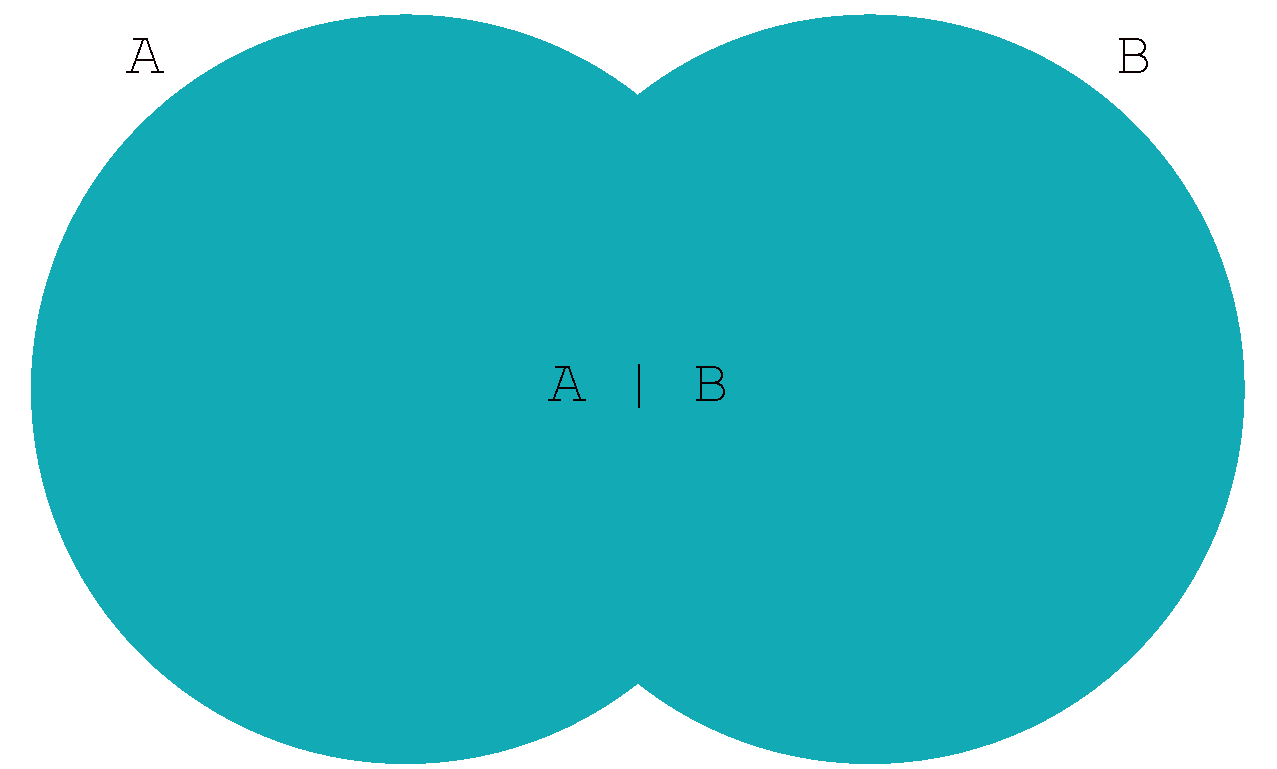
\includegraphics[width=0.45\linewidth]{img/mnozice2.pdf}\\
    \end{tabular}
    \caption{Vennova diagrama, ki ponazarjata osnovne operacije nad množicami. Slika na levi prikazuje razliko (\texttt{A-B} in \texttt{B-A}) in presek (\texttt{A \& B}) med množicama \texttt{A} in \texttt{B}. Slika na desni prikazuje unijo (\texttt{A | B}) med množicama \texttt{A} in \texttt{B}}
    \label{img:mnozice}
\end{figure}
Primer uporabe gornjih operacij je sledeč:
\begin{lstlisting}[language=Python]
>>> {1,2,3} & {3,4,5} # presek
{3}
>>> {1,2,3} | {3,4,5} # unija
{1,2,4,5}
>>> {1,2,3} - {3,4,5} # razlika
{1,2}
\end{lstlisting}

\section{Metode množic: dodajanje in brisanje elementov}
Dodajanje elementa v množico lahko izvedemo z uporabo metode \texttt{add}, ki kot argument sprejme element, ki ga želimo dodati:
\begin{lstlisting}[language=Python]
>>> mnozica = {1,2,3}
>>> mnozica.add(4)
>>> mnozica
{1, 2, 3, 4}
\end{lstlisting}
V primeru, da dodajamo element, ki v množici že obstaja, metoda ne naredi ničesar. Dodajanje bi lahko izvedli tudi z operatorjem \texttt{|=}, ki naredi unijo množice z neko drugo množico. V tem primeru lahko dodamo več elementov naenkrat:
\begin{lstlisting}[language=Python]
>>> mnozica = {1,2,3}
>>> mnozica |= {4,5}
>>> mnozica
{1, 2, 3, 4, 5}
\end{lstlisting}

Brisanje elementov iz množice vršimo z metodo \texttt{remove}. Ta v primeru neobstoja elementa vrne napako. Uporabimo lahko tudi metodo \texttt{discard}, ki v primeru neobstoja napake ne vrne, sicer pa deluje enako kot metode remove:
\begin{lstlisting}[language=Python]
>>> mnozica = {1,2,3}
>>> mnozica.remove(3)
>>> mnozica
{1, 2}
>>> mnozica.remove(3)
KeyError: 3
>>> mnozica.discard(2)
>>> mnozica
{1}
>>> mnozica.discard(2)
\end{lstlisting}
Podobno kot prej, lahko uporabimo tudi operator \texttt{-=}, ki naredi razliko med množico in neko drugo množico in to priredi izhodiščni množici:
\begin{lstlisting}[language=Python]
>>> mnozica = {1,2,3}
>>> mnozica -= {2,3}
>>> mnozica
{1}
\end{lstlisting}

\section{Zgled uporabe množic}
Ker so bili sprotni zgledi v tem poglavju relativno skopi, bomo to nadoknadili z malo daljšim zgledom, s katerim bomo povadili tudi slovarje in mogoče še kaj. 

Zamislimo si, da bi radi opazovali omrežje prijateljev oziroma povezanost ljudi preko relacije \emph{prijateljstvo}, bodisi v resničnem ali pa virtualnem življenju. Tako omrežje lahko predstavimo z \emph{neusmerjenim grafom}, v katerem vozlišča predstavljajo imena oseb, povezave med vozlišči pa prijateljstva med osebami. Te povezave so neusmerjene, saj prijateljstvo deluje v obe smeri: če je oseba 1 prijatelj osebe 2, je tudi oseba 2 prijatelj osebe 1. Primer grafa prijateljstev prikazuje slika \ref{img:prijatelji}.
\begin{figure}
    \centering
    \begin{tikzpicture}[scale=0.2]
        \tikzstyle{every node}+=[inner sep=0.5pt]
        \draw [black] (32.3,-4.5) circle (3);
        \draw (32.3,-4.5) node {Ana};
        \draw [black] (11.3,-20) circle (3);
        \draw (11.3,-20) node {Peter};
        \draw [black] (20,-28.5) circle (3);
        \draw (20,-28.5) node {Polona};
        \draw [black] (35.7,-23.1) circle (3);
        \draw (35.7,-23.1) node {Nejc};
        \draw [black] (49.3,-16.8) circle (3);
        \draw (49.3,-16.8) node {Janez};
        \draw [black] (12.706,-17.352) arc (148.85774:104.00397:27.119);
        %\fill [black] (29.35,-5.06) -- (28.46,-4.77) -- (28.7,-5.74);
        \draw [black] (21.37,-25.83) -- (30.93,-7.17);
        %\fill [black] (30.93,-7.17) -- (30.12,-7.65) -- (31.01,-8.11);
        \draw [black] (32.86,-24.08) -- (22.84,-27.52);
        %\fill [black] (22.84,-27.52) -- (23.76,-27.74) -- (23.43,-26.79);
        \draw [black] (46.87,-15.04) -- (34.73,-6.26);
        %\fill [black] (34.73,-6.26) -- (35.09,-7.13) -- (35.67,-6.32);
        \draw [black] (38.42,-21.84) -- (46.58,-18.06);
        %\fill [black] (46.58,-18.06) -- (45.64,-17.94) -- (46.06,-18.85);
        \draw [black] (49.578,-19.783) arc (-0.02318:-136.44145:16.075);
        %\fill [black] (49.58,-19.78) -- (49.08,-20.58) -- (50.08,-20.58);
        \draw [black] (50.395,-19.59) arc (17.2079:-187.5808:20.399);
        %\fill [black] (50.39,-19.59) -- (50.15,-20.5) -- (51.11,-20.21);
    \end{tikzpicture}
    \caption{Primer grafa omrežja prijateljstev.}
    \label{img:prijatelji}
\end{figure}

Da se bomo lahko lotili nadaljnjih analiz omrežja prijateljstev, moramo tega najprej prestaviti v obliko, ki jo bomo lahko zapisali v Pythonu. V nadaljevanju bomo napisali par funkcij, ki jih bomo lahko uporabili pri posodabljanju omrežja in njegovi analizi.

\begin{zgled}
Izberi si podatkovno strukturo, ki jo boš lahko uporabil pri predstavitvi in analizi omrežja prijateljstev ter z njo predstavi omrežje na sliki \ref{img:prijatelji}. Pri izbiri strukture upoštevaj to, da želiš nad omrežjem vršiti funkcije, kot so dodajanje prijateljev, brisanje prijateljev, iskanje skupnih prijateljev, iskanje osebe z največ prijatelji ipd.
\end{zgled}
\begin{resitev}
Omrežje bi lahko predstavili na različne načine, a vendar težimo k tisti predstavitvi, ki nam bo pri nadaljnjih operacijah nad omrežjem prihranila največ dela, hkrati pa bodo operacije nad omrežjem potekale kar se da hitro. Začnimo z mogoče najbolj intuitivno, a ne preveč dobro predstavitvijo, in sicer s seznamom terk. V tem primeru vsaka terka v seznamu vsebuje ime osebe in seznam njenih prijateljev. Omrežje s slike \ref{img:prijatelji} bi na tak način zapisali kot:
\begin{lstlisting}[language=Python]
prijatelji = [('Ana', ['Janez', 'Peter', 'Polona']),
              ('Janez', ['Ana', 'Nejc', 'Peter', 'Polona']),
              ('Nejc', ['Janez', 'Polona']),
              ('Peter', ['Ana', 'Janez']),
              ('Polona', ['Ana', 'Janez', 'Nejc'])]
\end{lstlisting}
Zakaj predstavitev ni najboljša? Zatakne se nam že pri izpisovanje vseh prijateljev podane osebe, saj že ta zahteva iskanje podane osebe s sprehodom čez (v najslabšem primeru) celoten seznam prijateljev. Če je ta seznam dolg, je lahko ta operacija časovno zelo potratna. Stvar bi lahko izboljšali, če bi namesto seznama terk uporabili kar slovar, v katerem so ključi imena oseb, vrednosti pa seznami prijateljev. Takole: 
\begin{lstlisting}[language=Python]
prijatelji = {'Ana': ['Janez', 'Peter', 'Polona'],
              'Janez': ['Ana', 'Nejc', 'Peter', 'Polona'],
              'Nejc': ['Janez', 'Polona'],
              'Peter': ['Ana', 'Janez'],
              'Polona': ['Ana', 'Janez', 'Nejc']}
\end{lstlisting}
S tem smo rešili problem iskanja prijateljev podane osebe, saj do teh pridemo z enostavnim indeksiranjem po imenu osebe, ki nas zanima. Še vedno pa je problematično npr. iskanje skupnih prijateljev dveh oseb, saj zahteva ugnezdeno zanko po seznamih prijateljev teh dveh oseb. Spet je ta operacija lahko časovno potratna, če so ti seznami dolgi, kar v socialnih omrežjih zagotovo ni izključeno. Temu problemu bi se lahko izognili tako, da prijatelje podane osebe predstavimo z množicami, nad katerimi so operacije kot je presek bolj učinkovite. Poleg tega glede na podan opis problema vrstni red prijateljev ni pomemben, posamezna oseba pa kot prijatelj druge osebe nastopa največ enkrat. Predstavitev bi bila torej sledeča:\begin{lstlisting}[language=Python]
prijatelji = {'Ana': {'Janez', 'Peter', 'Polona'},
              'Janez': {'Ana', 'Nejc', 'Peter', 'Polona'},
              'Nejc': {'Janez', 'Polona'},
              'Peter': {'Ana', 'Janez'},
              'Polona': {'Ana', 'Janez', 'Nejc'}}
\end{lstlisting}
\end{resitev}

\begin{zgled}
Napiši funkcijo \texttt{prijatelji\_od}, ki kot argument sprejme omrežje prijateljstev in ime osebe in izpiše vse prijatelje podane osebe. V primeru, da podane osebe ni v omrežju, naj funkcija to izpiše.
\end{zgled}
\begin{resitev}
Kot smo videli že prej, je zaradi izbrane predstavitve omrežja, iskanje prijateljev podane osebe enostavno. Preveriti moramo samo, če oseba v omrežju obstaja.
\begin{lstlisting}[language=Python,numbers=left]
def prijatelji_od(prijatelji, oseba):
    if oseba not in prijatelji: # ali je oseba v omrezju?
        print("Ta oseba ne obstaja!")
    else:
        print(prijatelji[oseba])
\end{lstlisting}
\end{resitev}

\begin{zgled}
Napiši funkcijo \texttt{dodaj\_osebo}, ki kot argument sprejme omrežje prijateljstev in ime osebe ter podano osebo doda v omrežje prijateljstev s prazno množico prijateljev.
\end{zgled}
\begin{resitev}
V omrežje bomo torej dodali novo osebo (nov ključ), na katerega bomo vezali prazno množico. Smiselno je tudi, da preverimo, če oseba v omrežju že obstaja. Ali mora funkcija vračati spremenjen slovar? Odgovor je seveda ne, saj je slovar spremenljiv podatkovni tip in se bo spreminjanje tega znotraj funkcije odražalo tudi izven funkcije.
\begin{lstlisting}[language=Python,numbers=left]
def dodaj_osebo(prijatelji, oseba):
    if oseba not in prijatelji: # dodaj samo, ce je se ni
        prijatelji[oseba] = set() # prazna mnozica
\end{lstlisting}
\end{resitev}

\begin{zgled}
Napiši funkcijo \texttt{spoprijatelji}, ki kot argument sprejme omrežje prijateljstev in imena dveh oseb, ki sta se spoprijateljili. Če sta osebi že v prijateljstvu, naj funkcija to izpiše. Če katerekoli izmed oseb še ni v omrežju, naj to osebo doda preko funkcije \texttt{dodaj\_osebo}.
\end{zgled}
\begin{resitev}
Spoprijateljevanje bomo naredili tako, da bomo prvo osebo dodali v množico prijateljev druge osebe in obratno. Pri tem lahko uporabimo metodo \texttt{add}. Še prej bomo po potrebi posamezno osebo dodali v omrežje, če je tam še ni.
\begin{lstlisting}[language=Python,numbers=left]
def spoprijatelji(prijatelji, oseba1, oseba2):
    if oseba1 not in prijatelji:
        dodaj_osebo(prijatelji, oseba1) 
    if oseba2 not in prijatelji:
        dodaj_osebo(prijatelji, oseba2) 
    
    # spoprijatelji samo, ce se nista prijatelja
    if oseba2 not in prijatelji[oseba1]:
        # dodaj oseba2 med prijatelje oseba1
        prijatelji[oseba1].add(oseba2)
        # dodaj oseba1 med prijatelje oseba2
        prijatelji[oseba2].add(oseba1)
    else:
        print("Osebi sta ze v prijateljstvu")
\end{lstlisting}
\end{resitev}

\begin{zgled}
Napiši funkcijo \texttt{skregaj}, ki kot argument sprejme omrežje prijateljstev in imena dveh oseb, ki sta se skregali. Če osebi nista v prijateljstvu, naj funkcija to izpiše. Če katerekoli izmed oseb še ni v omrežju, naj funkcija to izpiše. 
\end{zgled}
\begin{resitev}
Pri skreganju bomo prvo osebo odstranili iz množice prijateljev druge osebe in obratno. Pri tem lahko uporabimo metodo \texttt{remove}. Še prej bomo preverili, če osebi sploh sta v omrežju in če sta v relaciji prijateljstva.
\begin{lstlisting}[language=Python,numbers=left]
def skregaj(prijatelji, oseba1, oseba2):
    if oseba1 not in prijatelji or oseba2 not in prijatelji:
        print("Ene izmed oseb ni v omrezju!")
        return # koncaj in ne vrni nic
    # ce oseba1 ni prijatelj oseba2, velja tudi obratno
    if oseba1 not in prijatelji[oseba2]:    
        print("Osebi nista prijatelja!")
        return # koncaj in ne vrni nic
    
    # odstrani prijateljstvo
    prijatelji[oseba1].remove(oseba2)
    prijatelji[oseba2].remove(oseba1)
\end{lstlisting}
\end{resitev}

Zdaj pa se lotimo še analize omrežja.

\begin{zgled}
Napiši funkcijo \texttt{najbolj\_popularni}...
\end{zgled}
\begin{resitev}
...
\begin{lstlisting}[language=Python,numbers=left]

\end{lstlisting}
\end{resitev}

\begin{zgled}
Napiši funkcijo \texttt{najmanj\_popularni}...
\end{zgled}
\begin{resitev}
...
\begin{lstlisting}[language=Python,numbers=left]

\end{lstlisting}
\end{resitev}

\begin{zgled}
Napiši funkcije \texttt{skupni\_prijatelji}, \texttt{vsaj\_od\_enega} in \texttt{brez\_njegovih}...
\end{zgled}
\begin{resitev}
...
\begin{lstlisting}[language=Python,numbers=left]

\end{lstlisting}
\end{resitev}


\begin{zgled}
Napiši funkcijo \texttt{prijatelji\_prijateljev}...
\end{zgled}
\begin{resitev}
...
\begin{lstlisting}[language=Python,numbers=left]

\end{lstlisting}
\end{resitev}


\begin{zgled}
Napiši funkcijo \texttt{najvec_skupnih}...
\end{zgled}
\begin{resitev}
...
\begin{lstlisting}[language=Python,numbers=left]

\end{lstlisting}
\end{resitev}

\chapter{Oblikovanje nizov}

\section{Delo z nizi}

Nize smo do zdaj že dodobra spoznali. Preden se lotimo dela z datotekami pa si moramo pogledati še nekaj metod, ki jih lahko nad nizi uporabimo.

Ponovimo najprej osnovne operacije, ki smo jih do zdaj že izvajali nad nizi. Nad nizi lahko izvajamo zanko \texttt{for}, pri čemer v vsaki iteraciji zanke, dostopamo do enega znaka niza. Takole:
\begin{lstlisting}[language=Python]
>>> niz = "abeceda"
>>> for znak in niz:
	print(znak)
a
b
e
c
e
d
\end{lstlisting}
Nize lahko med sabo seštevamo, čemur smo rekli lepljenje ali konkatenacija, poleg tega pa jih lahko množimo s celimi števili:
\begin{lstlisting}[language=Python]
>>> "abc" + " " + "def"
'abc def'
>>> "abc" * 3
'abcabcabc'
\end{lstlisting}
Njihove elemente lahko tudi indeksiramo in delamo rezine. Ne moremo pa jih spreminjati. Odstranjevanje podniza z besedico \texttt{del} torej ne bo šlo skozi:
\begin{lstlisting}[language=Python]
>>> niz = "abeceda"
>>> niz[2:5]
'ece'
>>> del niz[2:5]
TypeError: 'str' object does not support item deletion
\end{lstlisting}
Zakaj ne? Ker so nizi nespremenljivi. Alternativa je seveda ta, da naredimo nov niz, ki odraža željeno spremembo. V zgornjem primeru bi torej lahko naredili nov niz z lepljenjem dveh rezin. Eno pred podnizom, ki ga želimo odstraniti, in drugo za podnizom, ki ga želimo odstraniti. Takole:
\begin{lstlisting}[language=Python]
>>> niz = "abeceda"
>>> niz[:2] + niz[5:]
'abda'
\end{lstlisting}
Iz niza smo tako odstranili podniz \texttt{"ece"}. Če želimo, da se sprememba odraža tudi preko spremenljivke z imenom \texttt{niz}, bomo nov (spremenjen) niz priredili temu imenu:
\begin{lstlisting}[language=Python]
>>> niz = "abeceda"
>>> niz = niz[:2] + niz[5:]
>>> niz
'abda'
\end{lstlisting}
Zapakirajmo vse skupaj v funkcijo.
\begin{zgled}
Napiši funkcijo \texttt{odstrani}, ki sprejme dva niza in iz prvega niza odstrani prvo pojavitev drugega niza ter spremenjen niz vrne. Če se drugi podniz v prvem ne pojavi, naj funkcija vrne nespremenjen niz.
\end{zgled}

\begin{resitev}
V funkciji moramo najprej preveriti, če in kje se v nizu nahaja podniz. To lahko naredimo tako, da se sprehajamo od začetka do konca niza in režemo rezine dolžine podniza. Da lahko delamo rezine, se moramo seveda sprehajati po indeksih niza. To bi izgledalo nekako takole:
\begin{lstlisting}[language=Python]
>>> niz = "abeceda"
>>> podniz = "ece"
>>> for i in range(len(niz)):
	niz[i:i+len(podniz)]
'abe'
'bec'
'ece'
'ced'
'eda'
'da'
'a'
\end{lstlisting}
Znotraj zanke bomo preverjali, če je odrezana rezina enaka podnizu (zgoraj je to bilo v 3. iteraciji zanke). V tem primeru ga bomo odstranili (podobno kot prej) in vrnili rezultat. Napišimo celotno funkcijo.
\begin{lstlisting}[language=Python,numbers=left]
def odstrani(niz, podniz):
    for i in range(len(niz)):
        rezina = niz[i:i+len(podniz)]
        if rezina == podniz:
            zacetek = i # začetek rezanja
            konec = i + len(podniz) # konec rezanja
            return niz[:zacetek] + niz[konec:]
    return niz # nismo našli - vrni nespremenjen niz
\end{lstlisting}
Vprašanje je še ali mora funkcija res vračati spremenjen niz ali je dovolj, če niz, ki ga funkcija sprejme kot argument, spreminjamo znotraj funkcije (kot smo to delali pri seznamih, slovarjih in množicah). Spremenjen niz moramo seveda eksplicitno vrniti, saj je niz nespremenljiv. Spremembe, ki jih vršimo nad imenom, za katerim se skriva niz, se izven funkcije ne bodo ohranile, zato je potrebno nov (spremenjen) niz vrniti s stavkom \texttt{return}. 
\end{resitev}

Tole je bilo še kar zakomplicirano. Izkaže pa se, da nam te in podobnih funkcij ni treba pisati, saj večinoma že obstajajo. Najdemo jih med metodami nizov. Izbrane (tj. tiste, ki jih bomo uporabljali pogosteje) si bomo podrobneje pogledali v nadaljevanju poglavja.

\section{Iskanje podnizov}
V prejšnjem zgledu se lahko uporabi rezin deloma izognemo z uporabo metode \texttt{startswith}, ki vrne vrednost \texttt{True}, če se niz, preko katerega smo metodo poklicali začne s podanim podnizom. Rešitev bi torej lahko nekoliko poenostavili:
\begin{lstlisting}[language=Python,numbers=left]
def odstrani(niz, podniz):
    for i in range(len(niz)):
        if niz[i:].startswith(podniz):
            zacetek = i # začetek rezanja
            konec = i + len(podniz) # konec rezanja
            return niz[:zacetek] + niz[konec:]
    return niz # nismo našli - vrni nespremenjen niz
\end{lstlisting}
Poleg metode \texttt{startswith} lahko pri iskanju uporabimo še metodo \texttt{endswith}, ki preverja, če se niz konča s podanim podnizom, metodo \texttt{count}, ki prešteje število pojavitev podniza in metodo \texttt{find}, ki vrne lokacijo podniza oziroma --1, če podniza v nizu ni. Povadimo še uporabo metode \texttt{find}:
\begin{lstlisting}[language=Python,numbers=left]
def odstrani(niz, podniz):
    i = niz.find(podniz)
    if i >= 0: # ali je podniz v nizu
        zacetek = i # začetek rezanja
        konec = i + len(podniz) # konec rezanja
        return niz[:zacetek] + niz[konec:]
    return niz
\end{lstlisting}

\section{Odstranjevanje in spreminjanje (pod)nizov}
Podnize pa lahko odstranimo zgolj s klicem metode \texttt{replace}, ki vse pojavitve prvega argumenta zamenja z drugim argumentom. Poskusimo
\begin{lstlisting}[language=Python]
>>> niz = "abeceda"
>>> niz.replace("a","e")
'ebecede'
\end{lstlisting}
Metoda podanega niza ne spreminja. Seveda, saj ga ne more, ker so nizi nespremenljivi. Metoda torej niza ne more spremeniti, lahko pa vrne nov niz, ki odraža spremembo. Če želimo s klicem metode spremeniti vrednost, ki stoji za imenom spremenljivke, bomo rezultat klica priredili spremenljivki. Takole:
\begin{lstlisting}[language=Python]
>>> niz = "abeceda"
>>> niz = niz.replace("a","e")
>>> niz
'ebecede'
\end{lstlisting}
Kako lahko uporabimo metodo pri odstranjevanju podnizov? Tako, da kot drugi argument podamo prazen niz.
\begin{lstlisting}[language=Python]
>>> niz = "abeceda"
>>> niz.replace("a","")
'beced'
\end{lstlisting}
V navodilu prejšnje naloge je bilo zahtevno, da odstranimo samo prvo pojavitev podniza. Tudi to lahko rešimo z dodatnim argumentom, ki ga metoda \texttt{replace} sprejema. Poglejmo si izpis funkcije \texttt{help}:
\begin{lstlisting}[language=Python]
>>> help("".replace)
Help on built-in function replace:

replace(old, new, count=-1, /) method of builtins.str instance
    Return a copy with all occurrences of substring old replaced
    by new.
    
      count
        Maximum number of occurrences to replace.
        -1 (the default value) means replace all occurrences.
    
    If the optional argument count is given, only the first count 
    occurrences are replaced.
\end{lstlisting}
Podamo lahko tudi tretji argument \texttt{count}, ki pove koliko zamenjav naj metoda naredi (privzeto naredi vse zamenjave). Zdaj lahko našo funkcijo poenostavimo do konca:
\begin{lstlisting}[language=Python,numbers=left]
def odstrani(niz, podniz):
    return niz.replace(podniz, "", 1)
\end{lstlisting}

Pogosto uporabljeni metodi za spreminjanje nizov sta še metodi \texttt{upper} in \texttt{lower}, ki spremenita vse črke niza v velike oziroma male. Ker Python loči med velikimi in malimi črkami, lahko ti dve metodi uporabimo, kadar te ločitve ne želimo imeti in vse pač spremenimo bodisi v velike bodisi v male črke. Povadimo na naslednjem zgledu.

\begin{zgled}
Napiši funkcijo \texttt{palindrom}, ki kot argument sprejme niz in vrne \texttt{True}, če je niz palindrom in \texttt{False}, če ni. Pri tem naj funkcija ne loči med malimi in velikimi črkami.
\end{zgled}

\begin{resitev}
Kako preveriti, če je niz palindrom, že znamo. Tokrat bomo dodali še to, da preverjanje ne loči med malimi in velikimi črkami. To bomo naredili tako, da bomo vse črke v nizu pred preverjanjem pretvorili v velike (ali pa v male).
\begin{lstlisting}[language=Python,numbers=left]
def palindrom(niz):
    niz = niz.upper()
    return niz == niz[::-1]
\end{lstlisting}
\end{resitev}

\section{Razdruževanje in združevanje nizov}
Funkcija \texttt{input} uporabnikov vnos vedno vrne zapisan kot niz. Prav tako bomo vsebino datotek (v naslednjem poglavju) vedno dobili najprej zapisano kot niz. V primeru, da uporabnik vnese eno število, lahko število zapisano kot niz enostavno pretvorimo preko funkcij \texttt{int} oziroma \texttt{float}. V primeru, da uporabnik naenkrat vnese več števil ali pa je vnos sestavljen iz števil in drugih znakov, ki jih mogoče želimo pretvoriti v kaj drugega pa ta pristop ni več mogoč. Deloma nas sicer lahko reši funkcija \texttt{eval}, katere uporaba zaradi varnosti v splošnem ni priporočljiva, poleg tega pa tudi ta slej ko prej odpove. V tem primeru moramo niz razčleniti \angl{parse} sami. Za ta namen lahko uporabimo metodo \texttt{split}, ki ji kot argument podamo ločilo \angl{separator}, preko katerega naj niz loči v seznam nizov. Poglejmo si primer:
\begin{lstlisting}[language=Python]
>>> niz = "jabolka,hruške,slive"
>>> niz.split(",")
['jabolka', 'hruške', 'slive']
\end{lstlisting}
Povadimo še na zgledu:

\begin{zgled}
Napiši program, ki na podlagi uporabnikovega vnosa izračuna in izpiše vsoto podanih števil. Uporabnik bo števila vnesel v eni vrstici in jih med seboj ločil s podpičji. 
\end{zgled}
\begin{resitev}
Program bo uporabnikov vnos (niz) ločil po podpičjih. Sledil bo sprehod čez dobljeni seznam, pretvorba nizov v števila in seštevanje.
\begin{lstlisting}[language=Python,numbers=left]
vnos = input("Vnesi števila ločena s podpičji: ")
seznam = vnos.split(";")
s = 0 # začetna vsota
for st in seznam:
    s += float(st) # pretvorba niza in prištevanje
print(s)
\end{lstlisting}
Zgled izvedbe programa:
\begin{lstlisting}[language=Python]
Vnesi števila ločena s podpičji: 20;40.5;60
120.5
\end{lstlisting}
\end{resitev}

Metodo \texttt{split} lahko pokličemo tudi brez podanega ločila, pri čemer bo privzeto za ločilo uporabljen \emph{prazen prostor} \angl{white space}. Prazen prostor predstavlja znake, ki na zaslonu predstavljajo točno to -- prazen prostor. Sem uvrstimo presledek, tabulator (\texttt{$\backslash$t}) in novo vrstico (\texttt{$\backslash$n}) (opomba: kombinacija znakov \texttt{$\backslash$t} in \texttt{$\backslash$n} pravzaprav predstavlja en sam znak). Dodatna prednost uporabe metode \texttt{split} brez argumenta je v tem, da bo več zaporednih ponovitev znakov za prazen prostor obravnaval kot eno samo. Poskusimo:
\begin{lstlisting}[language=Python]
>>> niz = "1    2 \n 3\t4"
>>> niz.split(" ")
['1', '', '', '', '2', '\n', '3\t4']
>>> niz.split()
['1', '2', '3', '4']
\end{lstlisting}
Klic metode z argumentom \texttt{" "} praznega prostora očitno ni odstranil v celoti, klic metode brez argumentov iz niza uspešno pobral samo relevantne vrednosti. 

Podobno, kot lahko podan niz glede na podano ločilo razbijemo na seznam nizov, lahko seznam nizov, glede na podano ločilo združimo v en niz. V tem primeru uporabimo metodo \texttt{join}, ki jo pokličemo nad nizom, ki predstavlja naše ločilo, kot argument pa ji podamo seznam nizov, ki ga želimo združiti. Takole: 
\begin{lstlisting}[language=Python]
>>> seznam = ["jabolka", "slive", "avokado"]
>>> ", ".join(seznam)
'jabolka, slive, avokado'
\end{lstlisting}


\section{Odstranjevanje \emph{praznega prostora}}

Dopolnimo najprej naše iskanje palindromov.
\begin{zgled}
Napiši funkcijo \texttt{palindrom}, ki kot argument sprejme niz in vrne \texttt{True}, če je niz palindrom in \texttt{False}, če ni. Pri tem naj funkcija ne loči med malimi in velikimi črkami, poleg tega pa naj ignorira presledke, znake za nove vrstice in tabulatorje.
\end{zgled}

\begin{resitev}
Želimo torej, da bi rešitev delovala tudi nad nečim takim kot je niz \texttt{"perica reže raci rep"}. Niz se prebere enako naprej kot nazaj, ampak samo v primeru, ko presledkov ne upoštevamo. Prva rešitev bo temeljila na tem, da vse bele prostore zamenjamo za prazne nize.
\begin{lstlisting}[language=Python,numbers=left]
def palindrom(niz):
    niz = niz.upper()
    niz = niz.replace(" ","")
    niz = niz.replace("\n","")
    niz = niz.replace("\t","")
    return niz == niz[::-1]
\end{lstlisting}
Alternativa je, da najprej nad nizom uporabimo metodo \texttt{split} brez podanega argumenta, ki bo niz ločila v seznam nizov, pri čemer bo odstranila ves prazen prostor. Zatem uporabimo metodo \texttt{join}, pri čemer kot ločilo uporabimo prazen niz. Takole:
\begin{lstlisting}[language=Python,numbers=left]
>>> niz = "perica \n reže \t raci rep"
>>> sez = niz.split()
>>> sez
['perica', 'reže', 'raci', 'rep']
>>> niz = "".join(sez)
>>> niz
'pericarežeracirep'
\end{lstlisting}
Druga rešitev je torej sledeča:
\begin{lstlisting}[language=Python,numbers=left]
def palindrom(niz):
    niz = niz.upper()
    sez = niz.split()
    niz = "".join(sez)
    return niz == niz[::-1]
\end{lstlisting}
Prve tri vrstice lahko združimo v eno:
\begin{lstlisting}[language=Python,numbers=left]
def palindrom(niz):
    niz = "".join(niz.upper().split())
    return niz == niz[::-1]
\end{lstlisting}
\end{resitev}

Beli prostor lahko torej odstranjujemo na različne načine. V določenih primerih pa želimo beli prostor odstraniti samo pred začetkom in po koncu \emph{prave} vsebine, vmes pa ne. V tem primeru lahko uporabimo metodo \texttt{strip}
\begin{lstlisting}[language=Python]
>>> niz = "\n   \t  Danes je lep dan!     \n"
>>> niz.strip()
'Danes je lep dan!'
\end{lstlisting}

%\section{Posebni znaki}

\section{Prilagajanje izpisa in formatiranje nizov}

Funkcija \texttt{print} podane argumente združi v niz, ki ga izpiše na zaslon. Pri tem med argumente vstavi presledke (\texttt{sep = " "}), na koncu izpisa pa gre v novo vrstico (\texttt{end = "$\backslash$n"}). Privzeto delovanje lahko spremenimo, tako da nastavimo (povozimo) privzete vrednosti izbirnima argumentom \texttt{sep} in \texttt{end}. 

Včasih pa to ni dovolj in bi bili radi z izpisovanjem nekoliko bolj ustvarjalni. V tem primeru lahko uporabimo metodo \texttt{format}. Metodo \texttt{format} pokličemo nad nizom, ki vsebuje t.~i. fiksne dele in dele, ki jih bo metoda zamenjala z argumenti, ki jih bomo podali ob klicu. Slednje znotraj niza označimo z zavitimi oklepaji (\texttt{\{} in \texttt{\}}). Osnovni primer uporabe je sledeč:
\begin{lstlisting}[language=Python]
>>> m = 1
>>> "{} meter/ov/a je {} centimeter/ov/a".format(m, m*100)
'1 meter/ov/a je 100 centimeter/ov/a'
\end{lstlisting}
Prvo pojavitev zavitega oklepaja je metoda \texttt{format} torej zamenjala s prvim argumentom, drugo pa z drugim. Znotraj zavitih oklepajev lahko tudi eksplicitno navedemo, kateri argument naj se uporabi pri zamenjavi. Takole:
\begin{lstlisting}[language=Python]
>>> m = 1
>>> "{0} m = {1} cm, torej je {1} cm = {0} m".format(m, m*100)
'1 m = 100 cm, torej je 100 cm = 1 m'
\end{lstlisting}
Do malo gršega izpisa pride, kadar imamo veliko decimalk:
\begin{lstlisting}[language=Python]
>>> cm = 12.673
>>> "{} cm = {} m".format(cm, cm/100)
'12.673 cm = 0.12673 m'
\end{lstlisting}
Rezultate lahko sicer zaokrožujemo z vgrajeno funkcijo \text{round}, ki ji kot argument podamo število decimalk. Alternativa je, da zaokroževanje podamo samo pri izpisu, tako da znotraj zavitih oklepajev malo bolj natančno povemo kako naj se izpis formatira. Takole:
\begin{lstlisting}[language=Python]
>>> cm = 12.673
>>> "{:5.1f} cm = {:5.2f} m".format(cm, cm/100)
' 12.7 cm =  0.13 m'
\end{lstlisting}
Kaj smo s tem povedali? Z dvopičjem povemo, da želimo izpis malo oblikovati. Število 5 podaja (najmanjše) število mest, ki naj jih izpis zasede. Iz izpisa je vidno, da je metoda format pred posamezno število vstavila presledek, saj je izpisano število dolgo 4 znake, mi pa smo povedali, da naj bo izpis dolg 5 znakov. Če bi bilo naše število daljše od 5 znakov, rezanja ne bi bilo, ampak bi \texttt{format} izpisal vse znake. Za piko smo podali število decimalk, ki naj bodo v izpisu. Pri centimetrih smo uporabili 1, pri metrih pa 2 decimalki. Oznaka \texttt{f} pomeni, da formatiramo decimalno število \angl{float}. Oblikovanje celih števil in nizov je enostavneje. V tem primeru podamo število mest, ki naj jih število (minimalno) zavzame. 
\begin{lstlisting}[language=Python]
>>> "{:3}: {:15}...{:5.2f}°C".format(1, "Ljubljana", 25.3)
'  1: Ljubljana      ...25.30°C'
\end{lstlisting}
Povemo lahko še ali naj se posamezen izpis poravna levo (\texttt{<}), desno (\texttt{>}) ali sredinsko (\texttt{\^}):
\begin{lstlisting}[language=Python]
>>> "{:<3}: {:<15}...{:>5.2f}°C".format(1, "Ljubljana", 25.3)
'1  : Ljubljana      ...25.30°C'
\end{lstlisting}
Presledke lahko zamenjamo tudi za kaj drugega, npr. za pike.
\begin{lstlisting}[language=Python]
>>> "{:<3}: {:.<15}...{:>5.2f}°C".format(1, "Ljubljana", 25.3)
'1  : Ljubljana.........25.30°C'
\end{lstlisting}
Zdaj lahko uporabo formatiranja demonstriramo na celotnem zgledu:
\begin{lstlisting}[language=Python]
>>> stevilke = [1,2,3]
>>> kraji = ["Ljubljana", "Maribor", "Nova Gorica"]
>>> temperature = [25.3, 21.32322, 26.433333]
>>> for st, kraj, temp in zip(stevilke, kraji, temperature):
	print("{:<3}: {:.<15}...{:>5.2f}°C".format(st, kraj, temp))
1  : Ljubljana.........25.30°C
2  : Maribor...........21.32°C
3  : Nova Gorica.......26.43°C
\end{lstlisting}

\section{Formatiranje nizov in \emph{f-Strings}}

Novejša in hitrejša alternativa metodi \texttt{format} je formatiranje nizov zapisanih v obliki, ki ji rečemo \emph{f-niz} oziroma \emph{f-Strings}. Tovrstne nize zapisujemo tako, da pred začetkom niza (pred navednice) zapišemo črko \texttt{f}. Python bo to razumel kot niz, ki ga mora še dodatno oblikovati. V osnovi tak niz zapišemo takole:
\begin{lstlisting}[language=Python]
>>> f'niz'
'niz'
\end{lstlisting}
V f-niz lahko v zavite oklepaje vstavimo spremenljivke, ki jih bo Python pri izpisu zamenjal za njihove vrednosti, podobno kot pri metodi \texttt{format}:
\begin{lstlisting}[language=Python]
>>> m = 1
>>> f"{m} meter/ov/a je {m*100} centimeter/ov/a"
'1 meter/ov/a je 100 centimeter/ov/a'
\end{lstlisting}
Tak način oblikovanja je nekoliko hitrejši kot oblikovanje z metodo \texttt{format}, predvsem pa je tak način oblikovanja bolj pregleden. Podobno kot pri metodi \texttt{format} lahko v zavite oklepaje podamo oblikovanje izpisa posamezne spremenljivke, le da je v tem primeru vrstni red malenkost drugačen, saj spremenljivko podamo kar v zavite oklepaje pred načinom njenega oblikovanja:
\begin{lstlisting}[language=Python]
f"{spremenljivka:oblikovanje}"
\end{lstlisting}
Poskusimo na zgledu:
\begin{lstlisting}[language=Python]
>>> cm = 12.673
>>> f"{cm:5.1f} cm = {cm/100:5.2f} m"
' 12.6 cm =  0.13 m'
\end{lstlisting}
Ostalo je zelo podobno oziroma enako kot pri uporabi metode \texttt{format}. Poskusimo še na zadnjem zgledu iz prejšnjega razdelka:
\begin{lstlisting}[language=Python]
>>> stevilke = [1,2,3]
>>> kraji = ["Ljubljana", "Maribor", "Nova Gorica"]
>>> temperature = [25.3, 21.32322, 26.433333]
>>> for st, kraj, temp in zip(stevilke, kraji, temperature):
	print(f"{st:<3}: {kraj:.<15}...{temp:>5.2f}°C")
1  : Ljubljana.........25.30°C
2  : Maribor...........21.32°C
3  : Nova Gorica.......26.43°C
\end{lstlisting}
Rezultat je torej enak kot v primeru uporabo metode \texttt{format}, je pa koda postala nekoliko krajša in bolj pregledna.
\chapter{Delo z datotekami}

\section{Zakaj pisati v datoteke in brati iz njih?}

Programi, ki smo jih napisali do zdaj, so podatke hranili le za čas njihovega izvajanja v t.i. \emph{delovnem pomnilniku}. Ko se je nek program končal, so ti podatki izginili in ko smo program ponovno zagnali, smo morali te podatke ponovno zgenerirati, npr. tako, da smo jih prebrali od uporabnika (če smo bolj natančni, so podatki izginili, ko smo resetirali okolje IDLE npr. z zagonom drugega ali istega programa). Ko smo torej dopolnjevali telefonski imenik z novimi vnosi, se je imenik ob končanju programa izbrisal in dodani vnosi so izginili. To običajno predstavlja problem zaradi več razlogov:
\begin{itemize}
    \item Ko se program neha izvajati, podatki izginejo. V primeru imenika se ta torej ob vsakem ponovnem zagonu programa resetira na začetno, npr. prazno, vsebino.
    \item Nimamo varnostnih kopij podatkov. Če se npr. telefon, ki uporablja naš imenik, ugasne, moramo celotno vsebino imenika ustvariti od začetka.
    \item Podatkov, ki smo jih ustvarili v enem programu, ne moremo oziroma težko uporabljamo v drugih programih. 
\end{itemize}
Na srečo lahko podatke v svojih programih iz delovnega pomnilnika oziroma iz vsebine spremenljivk, kadarkoli shranimo v t.i. \emph{trajni pomnilnik} oziroma po domače na \emph{disk}. S tem omogočimo njihovo trajno hrambo, kar pomeni, da lahko do teh podatkov pridemo tudi po zaključku izvajanja programa, na disku podatki ostanejo tudi po izklopu računalnika, do njih pa lahko pridemo tudi iz drugih programov. 

Kako pa podatke shranimo na disk? Podobno, kot smo do zdaj na disk shranjevali naše programe v obliki datotek s končnico \texttt{py}, lahko v (druge) datoteke shranjujemo tudi podatke, s katerimi delamo. 

Tako shranjene datoteke lahko kasneje v svojih programih preberemo in s tem \emph{obnovimo} stanje svojega delovnega pomnilnika oziroma določimo vrednosti spremenljivk na podlagi vsebine datoteke. Dodatna prednost branja podatkov iz datotek je to, da se nam zdaj ni treba več zanašati na vnos podatkov s strani uporabnika, ampak lahko podatke, ki jih želimo obdelati, v svoje programe preberemo kar iz datotek. Če bi npr. želeli pregledati podatke o povprečnih mesečnih plačah v Sloveniji, najpogostejših imenih ali inflaciji, bi te lahko prenesli iz spletne strani Statističnega urada republike Slovenije (SURS, \url{https://www.stat.si/statweb}), jih v svojem programu prebrali in ustrezno obdelali. V tem poglavju si bomo pogledali kako podatke iz datoteke prebrati in kako v datoteko podatke zapisati.

\section{Kaj je datoteka?}

Datoteke predstavljajo osnovni način zapisovanja podatkov na disku (ali na kakšnem drugem mediju). Datoteke predstavljajo trajno hrambo podatkov, omogočajo prenašanje podatkov med različnimi uporabniki in lahko vsebujejo različne tipe podatkov od teksta, besedil, slik in filmov, do datotek, ki jih operacijskih sistem uporablja za svoje delovanje. Ponavadi tip datoteke označuje njena končnica. Programi v Pythonu na primer uporabljajo končnico \texttt{py}, slike pa končnice kot \texttt{jpg}, \texttt{png} ali \texttt{gif}. 

V grobem lahko datoteke ločimo v dve skupini, in sicer na \emph{tekstovne datoteke} in \emph{binarne datoteke}. V obeh primerih vsebino datoteke predstavlja zaporedje števil, ki si jih lahko v primeru tekstovnih datotek interpretiramo kot zaporedje znakov oziroma nek (neoblikovan) tekst. Primer tekstovne datoteke je recimo datoteka s končnico \texttt{py} ali datoteka s končnico \texttt{txt}. Za tekstovne datoteke velja, da jih lahko odpremo z beležnico ali beležnici podobnimi orodji (npr. \emph{Notepad++}) in je njihova vsebina bolj ali manj berljiva. Kaj pa binarne datoteke? V skupino binarnih datotek uvrščamo vse ostalo, npr. slike, filme in oblikovana besedila. Če poskusite z beležnico odpreti datoteko s končnico \texttt{docx} (besedilo oblikovano z orodjem Microsoft Word), boste hitro videli, da to ni tekstovna datoteka. Tako kot pri tekstovnih datotekah je zapis s števili uporabljen tudi pri binarnih datotekah. Različna je le interpretacija teh števil. Medtem, ko lahko vsebino tekstovnih datotek orodja, kot je beležnica, enostavno dekodirajo kot zaporedje znakov, potrebujemo za binarne datoteke druga orodja oziroma programe, ki znajo njihovo vsebino dekodirati, glede na tip zapisa. Ena orodja pretvarjajo številke v slike, druga v filme, tretja v oblikovano besedilo. Katero orodje bo posamezno datoteko ob dvojnem kliku nanju odprlo, določa njena končnica. Če se končnica datoteke ne ujema z njeno vsebino, bo orodje vrnilo napako ali pa v najboljšem primeru prikazalo nekaj nenavadnega, podobno kot če datoteko s končnico \texttt{docx} odpremo z beležnico. 

\section{Tekstovne datoteke}
Tekstovne datoteke torej vsebujejo neoblikovan tekst, ki lahko predstavlja na primer neko besedilo, program v Pythonu ali pa podatke, ki smo jih zgenerirali tekom delovanja našega programa. V okviru spoznavanja osnov programiranja se bomo neposredno ukvarjali zgolj s tekstovnimi datotekami. 

\section{Odpiranje datoteke}

Če želimo neko datoteko v našem programu prebrati ali vanjo pisati, jo moramo najprej seveda odpreti. To lahko naredimo z vgrajeno funkcijo \texttt{open}, ki ji bomo za začetek podali zgolj ime datoteke, do katere želimo dostopati. Naredimo tekstovno datoteko \texttt{stevila.txt} s sledečo vsebino\footnote{Datoteko naredimo tako, da odpremo beležnico, vpišemo vsebino datoteke in datoteko shranimo.}:
\begin{lstlisting}[showstringspaces=false,numbers=left]
4
5.6
2
100
15
\end{lstlisting}
Datoteko shranimo v mapo kamor pač najpogosteje shranjujemo svoje datoteke. Zdaj jo poskusimo odpreti v Pythonu:
\begin{lstlisting}[language=Python, showstringspaces=false]
>>> open('stevila.txt')
FileNotFoundError: [Errno 2] No such file or directory: 
'stevila.txt'
\end{lstlisting}
Python pravi, da datoteke ne najde, čeprav smo jo pravkar ustvarili. Problem je v tem, da Python datoteko išče v svoji trenutni \emph{delovni mapi}, ki očitno ni enaka tisti, kamor smo mi shranili svojo datoteko\footnote{Do trenutne delovne mape lahko pridemo preko funkcije \texttt{getcwd} iz vgrajenega modula \texttt{os}.}. Problem bi lahko rešili na dva načina.

Prvi način je, da Pythonu podamo \emph{absolutno pot} do lokacije datoteke. Pythonu smo do datoteke v gornjem primeru podali t.i. \emph{relativno pot}, kar pomeni, da bo datoteko iskal relativno glede na trenutno delovno mapo. Če je njegova delovna mapa npr. \texttt{C:$\backslash$Windows$\backslash$system32}, pričakuje, da se datoteka nahaja tu. Lahko pa Pythonu podamo celotno oziroma \texttt{absolutno} pot. Če smo datoteko npr. shranili v mapo \texttt{C:$\backslash$Programiranje}, jo zdaj lahko odpremo takole:
\begin{lstlisting}[language=Python, showstringspaces=false]
>>> open('C:\\Programiranje\\stevila.txt')
<_io.TextIOWrapper name='C:\\Programiranje\\stevila.txt' mode='r'
encoding='cp65001'>
\end{lstlisting}
Tokrat smo datoteko le našli. Mimogrede, zakaj je bilo pri podajanju poti potrebno podati dve poševnici (\texttt{$\backslash$}). Kot smo videli v prejšnjem poglavju, poševnico Python obravnava kot začetek posebnega znaka. Z njo lahko npr. zapišemo tabulator (\texttt{$\backslash$t}) ali pa znak za novo vrstico (\texttt{$\backslash$n}). Če bi radi zapisali poševnico pa v niz enostavno vpišemo dve poševnici (\texttt{$\backslash\backslash$}).

Drugi način, ki je nekoliko enostavnejši in bolj pogost, je, da pač spremenimo svojo delovno mapo in potem do datoteke podamo relativno pot. To ponavadi v praksi pomeni, da podamo samo ime datoteke (kot v primeru, ko je Python javil napako). Kako pa spremenimo trenutno delovno mapo? Načeloma nam za to ni potrebno posebej skrbeti, saj bo IDLE ob zagonu programa Pythonovo delovno mapo avtomatsko zamenjal za tisto, v kateri se program nahaja. Če bomo datoteko odprli iz programa, ki se bo nahajal v isti mapi kot datoteka, lahko torej podamo zgolj njeno ime. Če torej naredimo program \texttt{branje.py} in ga shranimo v mapo, v katero smo prej shranili \texttt{stevila.txt}, lahko iz njega datoteko odpremo takole:
\begin{lstlisting}[language=Python, showstringspaces=false]
open('stevila.txt')
\end{lstlisting}

\section{Branje datoteke}
Datoteko smo torej uspešno odprli, zdaj pa jo bomo poskusili prebrati. Dostopanje do datoteke lahko izvedemo preko objekta, ki ga vrne funkcija \texttt{read}. Če hočemo datoteko prebrati, moramo ta objekt torej shraniti v neko spremenljivko, preko katere ga bomo lahko kasneje še poklicali. Takole:
\begin{lstlisting}[language=Python, showstringspaces=false]
f = open('stevila.txt')
\end{lstlisting}
Do metod za delo z datoteko lahko zdaj dostopamo preko spremenljivke \texttt{f}. Prvi način za branje datoteke je uporaba metode \texttt{read}, ki prebere datoteko od začetka do konca in vrne niz z njeno vsebino. V našem primeru bo rezultat sledeč:
\begin{lstlisting}[language=Python, showstringspaces=false]
>>> f.read()
'4\n5.6\n2\n100\n15'
\end{lstlisting}
To je torej zapisano v datoteki. Niz vsebuje števila, ki so med seboj ločena z znaki za novo vrstico \texttt{$\backslash$n}. Če bi želeli imeti lepši izpis, bi stvar izpisali s funkcijo \texttt{print}, ki znake za novo vrstico izpiše kot nove vrstice. Poskusimo:
\begin{lstlisting}[language=Python, showstringspaces=false]
>>> print(f.read())

\end{lstlisting}
Zakaj se tokrat ni nič izpisalo? Poleg tega, da lahko preko spremenljivke \texttt{f} dostopamo do datoteke, le-ta beleži, do kje je bila datoteka že prebrana. Datoteko lahko namreč beremo tudi po kosih (npr. vrstico po vrstico), pri čemer nočemo, da bi vedno brali npr. samo prvo vrstico, ampak bi radi slej ko prej prišli do konca datoteke. Ker smo našo datoteko že prebrali, jo moramo za ponovno branje ponovno odpreti. Ker je trenutna delovna mapa zdaj že enaka mapi, kjer se nahaja naša datoteka, lahko odpiranje tokrat naredimo kar iz ukazne vrstice:
\begin{lstlisting}[language=Python, showstringspaces=false]
>>> f = open('stevila.txt')
>>> print(f.read())
4
5.6
2
100
15
\end{lstlisting}

Že prej smo omenili, da lahko datoteko beremo tudi po vrsticah. Lahko npr. uporabimo metodo \texttt{readline}:
\begin{lstlisting}[language=Python, showstringspaces=false]
>>> f.readline()
''
\end{lstlisting}
Tole spet ne deluje, ker se nahajamo na koncu datoteke. Ponovno jo odprimo in preberimo prvo vrstico:
\begin{lstlisting}[language=Python, showstringspaces=false]
>>> f = open('stevila.txt')
>>> f.readline()
'4\n'
\end{lstlisting}
Branje po vrsticah lahko izvedemo tudi z zanko \texttt{for}. Takole:
\begin{lstlisting}[language=Python, showstringspaces=false]
>>> for vrstica in f:
	print(vrstica)
5.6

2

100

15
\end{lstlisting}
Prva vrstica seveda manjka, ker smo jo prej prebrali že z metodo \texttt{readline}. Zakaj se v izpisu pojavlja prazna vrstica? En znak za prazno vrstico je prispevala funkcija \texttt{print}, drugega pa smo dobili iz prebrane datoteke. Znake za prazno vrstico lahko iz niza, ki predstavlja trenutno prebrano vrstico, odstranimo z metodo \texttt{strip}, ki odstrani prazen prostor pred začetkom in po koncu \emph{prave} vsebine niza:
\begin{lstlisting}[language=Python, showstringspaces=false]
>>> f = open('stevila.txt')
>>> for vrstica in f:
	print(vrstica.strip())
4
5.6
2
100
15
\end{lstlisting}

Zadnja metoda, preko katere lahko preberemo datoteko, je metoda \texttt{readline}, ki podobno kot metoda \texttt{read} prebere celo datoteko, jo razbije po vrsticah in te zapiše v seznam.
\begin{lstlisting}[language=Python, showstringspaces=false]
>>> f = open('stevila.txt')
>>> f.readlines()
['4\n', '5.6\n', '2\n', '100\n', '15']
\end{lstlisting}

Datoteko lahko torej preberemo na več različnih načinov, pri čemer je vsem skupno to, da vsebino datoteke preberejo kot niz. Če bi želeli vsebino obravnavati kot kaj drugega, jo bomo morali prej ustrezno obdelati (podobno kot moramo npr. v ustrezen podatkovni tip pretvoriti rezultat funkcije \texttt{input}).

Poskusimo branje na zgledu.
\begin{zgled}
Napiši funkcijo \texttt{povprecje}, ki kot argument prejme niz z imenom datoteke in izračuna povprečje števil, ki so shranjena v datoteki. Predpostavljaš lahko, da je vsako število v datoteki zapisano v svoji vrstici. V primeru, da je datoteka prazna, naj funkcija vrne število 0.
\end{zgled}
\begin{resitev}
Funkcijo lahko napišemo s sprehodom čez vrstice, pri čemer vsebino vsake vrstice prištevamo skupni vsoti, ki jo na koncu delimo s številom vrstic. Vsebino vrstice moramo prej seveda očistiti (metoda \texttt{strip}) in pretvoriti v število (funkcija \texttt{float}). 
\begin{lstlisting}[language=Python, showstringspaces=false,numbers=left]
def povprecje(ime_datoteke):
    f = open(ime_datoteke)
    s = 0
    n = 0
    for vrstica in f:
        stevilo = float(vrstica.strip())
        s += stevilo
        n += 1
    if n > 0:
        return s/n
    else:
        return 0
\end{lstlisting}
\end{resitev}

Kaj pa če bi imeli v eni vrstici več števil? V tem primeru je potrebno vrstico več števil prej še razbiti na posamezna števila. To lahko naredimo z uporabo metode \texttt{split}, ki jo pokličemo nad posamezno vrstico in ji kot argument podamo ustrezno ločilo.

\begin{zgled}
Napiši funkcijo \texttt{povprecje}, ki kot argument prejme niz z imenom datoteke in izračuna povprečje števil, ki so shranjena v datoteki. Predpostavljaš lahko, da je v posamezni vrstici lahko zapisano več števil, ki so med seboj ločena z vejicami.
\end{zgled}
\begin{resitev}
Tokrat bomo posamezno vrstico z metodo \texttt{split} razbili na seznam, čez katerega se bomo sprehodili z ugnezdeno zanko \texttt{for}. Še vedno pa moramo posamezen element tega seznama pred prištevanjem skupni vsoti pretvoriti v število.
\begin{lstlisting}[language=Python, showstringspaces=false,numbers=left]
def povprecje(ime_datoteke):
    f = open(ime_datoteke)
    s = 0
    n = 0
    for vrstica in f:
        vrstica = vrstica.strip()
        for element in vrstica.split(","):
            stevilo = float(element)
            s += stevilo    
            n += 1
    if n > 0:
        return s/n
    else:
        return 0
\end{lstlisting}
\end{resitev}

Poskusimo rešiti še težave, ki smo jih imeli s telefonskim imenikom (pa tega nismo vedeli).
\begin{zgled}
Napiši funkcijo \texttt{preberi\_imenik}, ki kot argument prejme niz z imenom datoteke, ki vsebuje varnostno kopijo telefonskega imenika. Funkcija naj datoteko prebere in vrne slovar, v katerem so ključi imena oseb, vrednosti pa njihove telefonske številke zapisane kot nizi. Predpostavljaš lahko, da so podatki v datoteki zapisani v obliki \texttt{CSV}\footnote{CSV zapis \angl{comma separated values} predstavlja način zapisovanja podatkov v tekstovne datoteke, pri čemer vsaka vrstica vsebuje svoj zapis (npr. osebo), podatki znotraj posamezne vrstice (npr. ime osebe in telefonska številka) pa so med seboj ločeni z vejicami ali kakšnim drugim ločilom, kot je npr. podpičje ali tabulator. Pomembno je, da je za ločilo uporabljen znak, ki se sicer med podatki nikoli ne pojavi. Če bi npr. datoteka vsebovala decimalna števila ločena s piko, bi bila pika zelo slaba izbira za ločilo med podatki znotraj vrstice.}, pri čemer posamezna vrstica vsebuje ime osebe, ki je od telefonske številke osebe ločeno z vejico.
\end{zgled}
\begin{resitev}
Podobno kot v prejšnjem zgledu bomo s posamezno vrstico naredili sledeče:
\begin{itemize}
    \item odstranili bomo znak za novo vrstico z metodo \texttt{strip};
    \item vrstico bomo razbili na seznam nizov glede na uporabljeno ločilo (\texttt{','}) z metodo \texttt{split};
    \item seznam nizov bomo razpakirali in uporabili kot veleva navodilo naloge.
\end{itemize}

\begin{lstlisting}[language=Python, showstringspaces=false,numbers=left]
def preberi_imenik(ime_datoteke):
    f = open(ime_datoteke)
    imenik = {} # prazen slovar
    for vrstica in f:
        vrstica = vrstica.strip() # odstrani '\n'
        seznam = vrstica.split(',')
        ime = seznam[0]
        stevilka = seznam[1]
        imenik[ime] = stevilka # dodajanje vnosa
    return imenik
\end{lstlisting}
Funkcijo bi lahko še nekoliko izboljšali. Podobno, kot lahko razpakiramo terke, lahko razpakiramo tudi sezname. Torej lahko spremenljivkama \texttt{ime} in \texttt{stevilka} vrednosti priredimo kar v eni vrstici:
\begin{lstlisting}[language=Python, showstringspaces=false]
ime, stevilka = vrstica.split(',')
\end{lstlisting}
Če želimo, da funkcija deluje, tudi v primeru, ko datoteka vsebuje prazne vrstice, moramo pred obdelavo posamezne vrstice preveriti, če ta slučajno ni prazna. Po odstranjevanju znaka za novo vrstico torej preverimo neenakost s praznim nizom:
\begin{lstlisting}[language=Python, showstringspaces=false]
if vrstica != '':
\end{lstlisting}
To lahko krajše zapišemo kar takole:
\begin{lstlisting}[language=Python, showstringspaces=false]
if vrstica:
\end{lstlisting}
Zapišimo celotno rešitev:
\begin{lstlisting}[language=Python, showstringspaces=false,numbers=left]
def preberi_imenik(ime_datoteke):
    f = open(ime_datoteke)
    imenik = {} # prazen slovar
    for vrstica in f:
        vrstica = vrstica.strip() # odstrani '\n'
        if vrstica: # vrstica ni prazna?
            ime, stevilka = vrstica.split(',') # razpakiraj
            imenik[ime] = stevilka # dodajanje vnosa
    return imenik
\end{lstlisting}
\end{resitev}

\section{Pisanje v datoteko}

Pisanje v datoteko lahko izvedemo z metodo \texttt{write}, ki ji kot argument podamo niz, ki ga želimo v datoteko zapisati. Poskusimo:
\begin{lstlisting}[language=Python, showstringspaces=false]
>>> f = open('stevila.txt')
>>> f.write(6)
TypeError: write() argument must be str, not int
\end{lstlisting}
Ravnokar smo rekli, da moramo metodi \texttt{write} podati \textbf{niz}, ki ga želimo zapisati. Če hočemo torej v datoteko zapisati število, ga moramo prej pretvoriti v niz s funkcijo \texttt{str}. Poskusimo še enkrat: 
\begin{lstlisting}[language=Python, showstringspaces=false]
>>> f = open('stevila.txt')
>>> f.write('6')
io.UnsupportedOperation: not writable
\end{lstlisting}
Tokrat smo dobili drugo napako. Vidimo, da pisanje ni mogoče, ker smo datoteko odprli za branje. Več informacij o odprti datoteki, lahko izvemo preko spremenljivke, v katero smo datoteko odprli:
\begin{lstlisting}[language=Python, showstringspaces=false]
>>> f
<_io.TextIOWrapper name='stevila.txt' mode='r' encoding='cp65001'>
\end{lstlisting}
Iz izpisa vidimo, da smo odprli datoteko z imenom \texttt{'stevila.txt'} (kar že vemo) in da je \texttt{mode} oziroma način odpiranja datoteke enak vrednosti \texttt{'r'}, ki se nanaša na branje oziroma \emph{read}. Način odpiranja datoteke lahko funkciji \texttt{open} nastavimo z izbirnim argumentom \texttt{mode}, ki je privzeto enak vrednosti \texttt{'r'}. Če argumenta ne nastavimo, bomo torej datoteko odprli za branje. Pogosto uporabljena načina odpiranja datoteke sta še \texttt{'w'} oziroma pisanje \angl{write} in \texttt{'a'} dodajanje \angl{append}. Pisanju bi lahko, če bi bili nekoliko bolj natančni, rekli tudi prepisovanje, saj bomo s takim načinom pisanja obstoječo datoteko prepisali. Dodajanju bi v podobnem kontekstu lahko rekli dopisovanje, saj bomo obstoječi datoteki vsebino dodajali (na koncu obstoječe vsebine). Pri obeh načinih pa zdaj napake, če datoteka s podanim imenom ne bo obstajala, ne bomo dobili, ampak bo Python to datoteko pač ustvaril. Poskusimo zdaj v datoteko \texttt{'stevila.txt'} zapisati par stevil. Najprej jo odpremo za pisanje:
\begin{lstlisting}[language=Python, showstringspaces=false]
>>> f = open('stevila.txt', mode = 'w')
\end{lstlisting}
Zdaj pa pišimo:
\begin{lstlisting}[language=Python, showstringspaces=false]
>>> f.write('1')
1
>>> f.write('2')
1
>>> f.write('3')
1
>>> f.write('45')
2
\end{lstlisting}
Vsakič, ko pokličemo metodo \texttt{'write'} ta vrne število znakov, ki smo jih zapisovali. Ko zdaj datoteko \texttt{stevila.txt} odpremo z beležnico (ali beležnici podobnim orodjem), vidimo, da je ta prazna. Zakaj? Pravilo lepega dela z datotekami je, da jih po vsakem odpiranju tudi zapremo za kar lahko uporabimo metodo \texttt{close}. Pri branju to ni nujno potrebno, saj se bo datoteka zaprla avtomatsko, ko bo iz našega imenskega prostora izginila spremenljivka, preko katere smo datoteko brali (najkasneje, ko bomo resetirali okolje IDLE). Pri pisanju pa se lahko zgodi, da bo vsebina datoteke brez eksplicitnega zapiranja datoteke ostala prazna. Ker je pisanje v datoteko počasna operacija, Python, kot smo že navajeni, to v določeni meri optimizira oziroma pohitri. Ko od njega zahtevamo pisanje v datoteko, namreč raje piše v medpomnilnik \angl{buffer}, katerega vsebino bo v dejansko datoteko Python zapisal bodisi takrat, ko se bo nabralo malo več podatkov, da se mu bo splačalo to zapisati v datoteko, ali pa takrat, ko bomo datoteko zaprli, saj s tem povemo, da vanjo ne bomo več pisali. Če želimo, da se naša števila v datoteko zagotvo zapišejo, jo moramo torej zapreti:
\begin{lstlisting}[language=Python, showstringspaces=false]
>>> f.close()
\end{lstlisting}
Ko zdaj odpremo datoteko, vidimo, da se je prejšnja vsebina datoteke prepisala -- seveda, saj smo datoteko odprli za prepisovanje. V njej vidimo sledečo vsebino:
\begin{lstlisting}[showstringspaces=false,numbers=left]
12345
\end{lstlisting}
To ni tisto kar smo hoteli? Mogoče ne, je pa to tisto, kar smo zahtevali. Metoda \texttt{write} namreč v datoteko zapiše točno tisto, kar od nje zahtevamo. Če bi želeli števila zapisati vsako v svojo vrstico, bi morali zraven vsakega števila zapisati tudi znak za novo vrstico (\texttt{$\backslash$n}). Takole:
\begin{lstlisting}[language=Python, showstringspaces=false]
>>> f.write('1')
ValueError: I/O operation on closed file.
\end{lstlisting}
Ker smo datoteko zaprli, zdaj vanjo ne moremo več pisati. Pred ponovnim pisanjem, jo moramo torej spet odpreti:
\begin{lstlisting}[language=Python, showstringspaces=false]
>>> f = open('stevila.txt', mode='w')
>>> f.write('1\n')
2
>>> f.write('2\n')
2
>>> f.write('3\n')
2
>>> f.write('45\n')
3
\end{lstlisting}
Datoteko moramo na koncu seveda spet zapreti
\begin{lstlisting}[language=Python, showstringspaces=false]
>>> f.close()
\end{lstlisting}
Zdaj je njena vsebina sledeča:
\begin{lstlisting}[showstringspaces=false,numbers=left,showlines=true]
1
2
3
45

\end{lstlisting}
Datoteka se konča s prazno vrstico, v katero smo skočili za nizom \texttt{45}. Dodajmo v datoteko še par števil. Če želimo v datoteko novo vsebino dodajati k obstoječi vsebini, jo moramo odpreti za dopisovanje (\texttt{mode='a'}).
\begin{lstlisting}[language=Python, showstringspaces=false]
>>> f = open('stevila.txt', mode='a')
>>> f.write('55\n')
3
>>> f.write('133\n')
4
>>> f.write('-6.98\n')
6
>>> f.close()
\end{lstlisting}
Ko datoteko ponovno odpremo z beležnico, vidimo, da smo v njej dobili tri nove vrstice:
\begin{lstlisting}[showstringspaces=false,numbers=left,showlines=true]
1
2
3
45
55
133
-6.98

\end{lstlisting}

Povadimo pisanje še na zgledu.
\begin{zgled}
Napiši funkcijo \texttt{nakljucna}, ki kot argument prejme niz z imenom datoteke in celo število, ki podaja število naključnih števil, ki naj jih funkcija zapiše v datoteko s podanim imenim. Funkcija naj v vsako vrstico v datoteki zapiše največ 10 naključnih celih števil iz intervala od 1 do 100.
\end{zgled}
\begin{resitev}
Naključna števila bomo generirali z uporabo funkcije \texttt{randint} modula \texttt{random}. V datoteko bomo pisali po eno število naenkrat. Po vsakem pisanju lahko zapišemo tudi presledek, na vsakih 10 pisanj pa bomo zapisali znak za novo vrstico.
\begin{lstlisting}[language=Python, showstringspaces=false,numbers=left]
# uvazanje vedno delamo izven funkcij
from random import randint

def nakljucna(ime_datoteke, n):
    f = open(ime_datoteke, mode='w') # odpri za prepisovanje
    for i in range(1,n+1): # zanko ponovimo n-krat
        st = randint(1,100) # naključno število od 1 do 100
        f.write(str(st)) # število moramo pretvoriti v niz
        if i % 10 == 0: # ali je čas za novo vrstico
            f.write('\n')
        else:
            f.write(' ')
    f.close()
\end{lstlisting}
\end{resitev}

Metoda \texttt{write} torej v datoteko zapiše točno tisto, kar ji podamo, vedno pa ji moramo podati točno en podatek tipa \texttt{str}. Če bi želeli naenkrat zapisati več podatkov, jih moramo torej pred tem sami združiti. V določenih primerih bi bilo veliko bolj priročno, če bi lahko v datoteko pisali na enak način, kot smo stvari izpisovali na zaslon, tj. s funkcijo \texttt{print}. Ta sprejema vrednosti poljubnega tipa, poleg tega pa ji lahko podamo več vrednosti, ki jih bo med sabo združila (privzeto z ločilom \texttt{' '}). Izkaže se, da lahko za pisanje v datoteke uporabimo tudi funkcijo \texttt{print}. Pri tej moramo opcijskemu argumentu z imenom \texttt{file} prirediti spremenljivko, v katero smo datoteko odprli\footnote{Opcijski argument \texttt{file} funkcije \texttt{print} je privzeto postavljen na vrednost \texttt{sys.stdout}, kar pomeni, da pišemo na standardni izhod -- v našem primeru je to konzola okolja IDLE.} Poskusimo na prejšnjem zgledu.
\begin{zgled}
Napiši funkcijo \texttt{nakljucna}, ki kot argument prejme niz z imenom datoteke in celo število, ki podaja število naključnih števil, ki naj jih funkcija zapiše v datoteko s podanim imenim. Funkcija naj v vsako vrstico v datoteki zapiše največ 10 naključnih celih števil iz intervala od 1 do 100. Za pisanje v datoteko uporabi funkcijo \texttt{print}.
\end{zgled}
\begin{resitev}
Rešitev je zelo podobna kot prej, le da nam tokrat števil ni potrebno pretvarjati v nize, funkcija \texttt{print} pa tudi sama poskrbi za pisanje presledkov in novih vrstic (le pravilno jo moramo poklicati).
\begin{lstlisting}[language=Python, showstringspaces=false,numbers=left]
# uvazanje vedno delamo izven funkcij
from random import randint

def nakljucna(ime_datoteke, n):
    f = open(ime_datoteke, mode='w') # odpri za prepisovanje
    for i in range(1,n+1): # zanko ponovimo n-krat
        st = randint(1,100) # naključno stevilo od 1 do 100
        if i % 10 == 0: # ali je čas za novo vrstico
            print(st, file=f) # nova vrstica
        else:
            print(st, end=' ', file=f) # presledek 
    f.close()
\end{lstlisting}
\end{resitev}

Za konec dopolnimo še zgled s telefonskim imenikom.
\begin{zgled}
Napiši funkcijo \texttt{shrani\_imenik}, ki kot argument prejme niz z imenom datoteke, ki naj vsebuje varnostno kopijo telefonskega imenika in slovar, v katerem so ključi imena oseb, vrednosti pa njihove telefonske številke. Funkcija imenik zapiše v datoteko s podanim imenom, in sicer tako, da vsaka vrstica vsebuje podatke o eni osebi, pri čemer je ime od telefonske številke ločeno z vejico, tako da bo izhod funkcije kompatibilen s funkcijo \texttt{preberi\_imenik}.
\end{zgled}
\begin{resitev}
V funkciji se bomo sprehodili čez cel imenik in v vsako vrstico zapisali ime in telefonsko številko. Takole:
\begin{lstlisting}[language=Python, showstringspaces=false,numbers=left]
def shrani_imenik(ime_datoteke, imenik):
    f = open(ime_datoteke, mode='w') # prepisovanje
    for ime, stevilka in imenik.items():
        f.write(ime) 
        f.write(',')
        f.write(stevilka)
        f.write('\n')
    f.close()
\end{lstlisting}
Štiri nize (\texttt{ime}, \texttt{','}, \texttt{stevilka} in \texttt{'$\backslash$n'} bi lahko združili skupaj in metodo \texttt{write} uporabili samo enkrat.
\begin{lstlisting}[language=Python, showstringspaces=false,numbers=left]
def shrani_imenik(ime_datoteke, imenik):
    f = open(ime_datoteke, mode='w') # prepisovanje
    for ime, stevilka in imenik.items():
        f.write(ime+','+stevilka+'\n')
    f.close()
\end{lstlisting}
Za pisanje pa bi lahko uporabili tudi funkcijo \texttt{print}. Tej moramo spremeniti privzeto ločilo (presledek) v zahtevano ločilo (vejica). Takole:
\begin{lstlisting}[language=Python, showstringspaces=false,numbers=left]
def shrani_imenik(ime_datoteke, imenik):
    f = open(ime_datoteke, mode='w') # prepisovanje
    for ime, stevilka in imenik.items():
        print(ime, stevilka, sep=',', file=f)
    f.close()
\end{lstlisting}
\end{resitev}

\section{Kodiranje znakov}

Že na začetku poglavja smo omenili, da vsebino datoteke predstavlja zaporedje števil, ki jih lahko v primeru tekstovnih datotek pretvorimo v neoblikovan tekst oziroma neko zaporedje znakov. Vsak znak je torej shranjen kot neko število. \emph{Kodiranje} določa preslikavo, ki posamezno število oziroma \emph{kodo} preslika v določen znak. Do kode znaka lahko pridemo z uporabo vgrajene funkcije \texttt{ord}, ki ji kot argument podamo en znak:
\begin{lstlisting}[language=Python, showstringspaces=false]
>>> ord('a')
97
>>> ord('A')
65
\end{lstlisting}
Preslikavo lahko naredimo tudi v drugo smer (iz kode v znak), in sicer z uporabo funkcije \texttt{chr}, ki ji kot argument podamo kodo znaka:
\begin{lstlisting}[language=Python, showstringspaces=false]
>>> chr(97)
'a'
>>> chr(65)
'A'
\end{lstlisting}

Koda posameznega znaka je torej odvisna od uporabljenega kodiranja. Izkaže se, da so osnovni znaki ne glede na uporabljeno kodiranje zakodirani na enak način. Pri kodiranju teh se namreč uporablja 7-bitni standard ASCII \angl{ American Standard Code for Information Interchange}. Za kodiranje posameznega znaka lahko torej uporabimo 7 bitov, kar pomeni, da lahko zakodiramo $2^7=128$ različnih znakov. Pri tem je 32 kod rezerviranih za posebne znake (med te sodi npr. tudi znak za novo vrstico), torej nam ostane 96 kod, s katerimi moramo predstaviti male črke, velike črke, številke in različna ločila ter simbole. Izkaže se, da teh kod zelo hitro zmanjka in zato služijo zgolj predstavitvi osnovnih znakov in črk angleške abecede. Kaj pa naši šumnik, nemški preglasi in kitajske pismenke? Za predstavitev teh moramo uporabiti razširitve kodiranja ASCII. Omenimo dve razširitvi, ki sta v pogosti uporabi v današnjem času. 

Kodne tabele \angl{code page} kodiranje ASCII razširjajo z dodatnim bitom, kar pomeni, da lahko z njihovo uporabo predstavimo dodatnih 128 znakov. To je sicer dovolj za znake č, ž in š, kaj pa za kitajske pismenke? Dodatnih kod seveda ni dovolj, da bi predstavili še te, poleg njih pa mogoče še črke iz cirilice, korejski hangul in še kaj drugega. Iz tega razloga se v različnih delih sveta uporabljajo različne kodne tabele. Pri nas je npr. v uporabi centralno-evropska kodna tabela \texttt{cp1250}, s katero lahko predstavimo tudi znake č, ž in š. Znak \texttt{č} je v tej kodni tabeli določen s kodo \texttt{232}. V Nemčiji uporabljajo zahodno-evropsko kodno tabelo \texttt{cp1252}, s katero sicer ne moremo predstaviti šumnikov, lahko pa predstavimo preglase.  V tej kodni tabeli koda \texttt{232} predstavlja znak \texttt{è}, kar ste mogoče že kdaj opazili, npr. pri predvajanju podnapisov.

Kljub temu, da se kodne tabele še vedno uporabljajo, je v današnjem času v večinski rabi standard \emph{unicode}, katerega pomemben predstavnik je kodiranje UTF-8. Pri tem je posamezen znak zapisan z minimalno 8 biti. V primeru, da se v našem besedilu pojavijo znaki, ki ne nastopajo v osnovnem ASCII kodiranju (npr. č), se zapis posameznega znaka razširi (V konkretnem primeru na 16-bitni zapis).

Zakaj se moramo s kodiranjem znakov ukvarjati v okviru osnov programiranja? Pri branju in pisanju datotek je zaželeno, da izrecno podamo kodiranje, ki ga želimo uporabiti. S tem se namreč izognemo težavam z napačno interpretacijo znakov. Če je nekdo zapisal datoteko z uporabo kodiranje UTF-8, mi pa jo poskusimo odpreti s kodiranjem cp1250, bo prišlo do napake ali pa bodo znaki dekodirani narobe. Če kodiranja ne podamo (kot ga nismo podali v primerih zgoraj), bo uporabljeno privzeto kodiranje našega operacijskega sistema. Poglejmo si še enkrat kaj se skriva za spremenljivko, preko katere odpremo datoteko:
\begin{lstlisting}[language=Python, showstringspaces=false]
>>> f = open('stevila.txt')
>>> f 
<_io.TextIOWrapper name='stevila.txt' mode='r' encoding='cp65001'>
\end{lstlisting}
Kodiranje \angl{encoding} je v konkretnem primeru nastavljeno na \texttt{'cp650010'}, ki predstavlja nekakšen ekvivalent kodiranja UTF-8 v operacijskem sistemu Windows. Operacijski sistem Windows sicer pogosto uporablja kodiranje cp1250, Linux pa UTF-8. Zmešnjava je torej popolna. To lahko povzroči nemalo težav, zato je pri delu z datotekami pomembno, da vedno podamo način kodiranja. Dogovorimo se, da bomo od zdaj naprej pri delu z datotekami vedno podali način kodiranja, ki naj bo kar UTF-8. 

Kodiranje, ki ga želimo uporabiti pri pisanju ali branju datoteke, navedemo pri odpiranju datoteke s funkcijo \texttt{open} preko izbirnega argumenta \texttt{encoding}. Zapišimo datoteko z uporabo kodiranja UTF-8\footnote{Argument \texttt{encoding} bomo nastavili na vrednost \texttt{'utf8'}, \texttt{'utf-8'}, \texttt{'UTF8'} ali \texttt{'UTF-8'}.}:
\begin{lstlisting}[language=Python, showstringspaces=false]
>>> f = open("posebni_znaki.txt", mode='w', encoding="utf8")
>>> f.write("čžš")
3
>>> f.close()
\end{lstlisting}
Zdaj datoteko preberimo z uporabo kodiranja cp1250:
\begin{lstlisting}[language=Python, showstringspaces=false]
>>> f = open("posebni_znaki.txt", encoding="cp1250")
>>> f.read()
'ÄŤĹľĹ'
\end{lstlisting}

Rezultat je seveda napačen. Poskusimo še s pravilnim kodiranjem:
\begin{lstlisting}[language=Python, showstringspaces=false]
>>> f = open("posebni_znaki.txt", encoding="utf8")
>>> f.read()
'čžš'
\end{lstlisting}

Izbira ustreznega kodiranja pri delu z datotekami je torej pomembna. Dopolnimo naši funkciji za branje telefonskega imenika iz datoteke in njegovo zapisovanje v datoteko, saj je velika verjetnost, da bodo v imenih naših prijateljev nastopali tudi šumniki.

\begin{zgled}
Napiši funkciji za branje in shranjevanje telefonskega imenika v in iz datoteke, pri čemer je imenik podan kot slovar, v katerem ključi predstavljajo imena oseb, vrednosti pa njihove telefonske številke. Datoteka naj bo zakodirana z uporabo kodiranja UTF-8.
\end{zgled}
\begin{resitev}
Rešitev bo praktično enaka kot v prej, le da bomo pri odpiranju datoteke izbirni argument \texttt{encoding} postavili na vrednost \texttt{'utf8'}.
\begin{lstlisting}[language=Python, showstringspaces=false,numbers=left]
def shrani_imenik(ime_datoteke, imenik):
    # pri odpiranju datoteke podamo še kodiranje
    f = open(ime_datoteke, mode='w', encoding='utf8')
    for ime, stevilka in imenik.items():
        print(ime, stevilka, sep=',', file=f)
    f.close()

def preberi_imenik(ime_datoteke):
    # pri odpiranju datoteke podamo še kodiranje
    f = open(ime_datoteke, encoding='utf8') 
    imenik = {} # prazen slovar
    for vrstica in f:
        vrstica = vrstica.strip() # odstrani '\n'
        if vrstica: # vrstica ni prazna?
            ime, stevilka = vrstica.split(',') # razpakiraj
            imenik[ime] = stevilka # dodajanje vnosa
    return imenik
\end{lstlisting}
\end{resitev}

\chapter{Vizualizacija podatkov}

\section{Knjižnica Matplotlib in njena namestitev}
Za vizualizacijo podatkov bomo uporabljali knjižnico Matplotlib, ki predstavlja osnovo za risanje kakršnihkoli grafov. Ker v osnovni različici jezika Python še ni nameščen, ga moramo pred uporabo namestiti (če imate nameščeno distribucijo Anaconda, imate to knjižnico že nameščeno). Kot smo spoznali v poglavju \ref{ch:moduli} lahko za namestitev knjižnice uporabimo orodje \texttt{pip}, tako da zaženemo ukazno vrstico svojega operacijskega sistema (ne okolja IDLE) in vanjo vpišemo
\begin{lstlisting}[language=bash]
> pip install matplotlib
\end{lstlisting}
Podrobnejša navodila za namestitev paketov smo podali že v poglavju \ref{ch:moduli}, zato jih tu ne bomo podvajali. Če ima vaš računalnik povezavo z internetom, bo orodje \texttt{pip} samo preneslo potrebne namestitvene datoteke in knjižnico namestilo.

Za vizualizacija naših podatkov bomo uporabili Matplotlibov vmesnik \angl{interface} \texttt{pyplot}, ki nam risanje precej olajša. V svoje programe ga bomo uvozili takole:
\begin{lstlisting}[language=Python, showstringspaces=false]
import matplotlib.pyplot as plt
\end{lstlisting}
Zdaj lahko do funkcij za risanje grafov dostopamo takole:
\begin{lstlisting}[language=Python, showstringspaces=false]
plt.ime_funkcije(argumenti)
\end{lstlisting}

\section{Funkciji \texttt{plot} in \texttt{show}}

Začeli bomo s funkcijo \texttt{plot}, ki omogoča izris črtnega grafa \angl{line plot}. V osnovi ji lahko podamo zgolj en seznam. Poskusimo:
\begin{lstlisting}[language=Python, showstringspaces=false]
>>> Y = [1, 3, 9, 12]
>>> plt.plot(Y)
[<matplotlib.lines.Line2D object at 0x000001DD7FB28860>]
\end{lstlisting}
Nekaj se je očitno zgodilo, grafa pa še vedno ne vidimo. Funkcija \texttt{plot} namreč deluje tako, da grafe riše v ozadju in te dodaja na risalno površino, ki pa jo pokaže, šele ko pokličemo funkcijo \texttt{show}.
\begin{lstlisting}[language=Python, showstringspaces=false]
>>> plt.show()
\end{lstlisting}
Zdaj se je pokazal graf, ki ga prikazuje slika \ref{img:plt1}.
\begin{figure}
    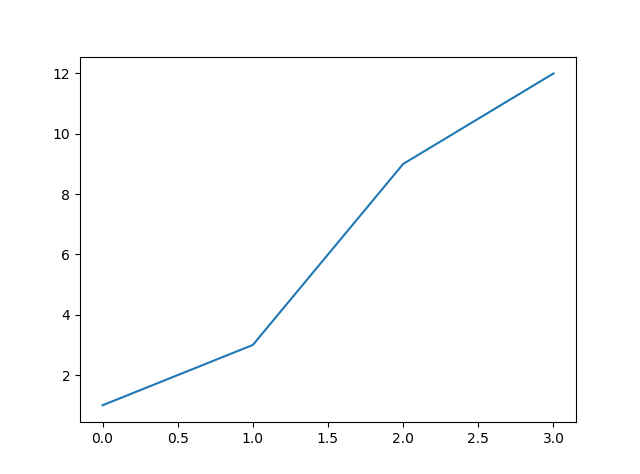
\includegraphics[width=\linewidth]{img/plt1.png}
    \caption{Črtni graf, pri čemer smo podali koordinate točk na osi $y$.}
    \label{img:plt1}
\end{figure}
Točke, ki smo jih podali funkciji \texttt{plot}, očitno predstavljajo koordinate $y$ narisanega grafa. Točke na osi $x$ je Matplotlib določil kar glede na indekse točke v seznamu \texttt{Y}. To lahko spremenimo, tako da funkcijo \texttt{plot} pokličemo z dvema seznamoma, pri čemer prvi določa koordinate točk na osi $x$ drugi pa koordinate točk na osi $y$. Seznama morata biti seveda enakih dolžin. Do enakega grafa kot zgoraj, bi lahko prišli takole: 
\begin{lstlisting}[language=Python, showstringspaces=false]
>>> Y = [1, 3, 9, 12]
>>> X = range(len(Y))
>>> plt.plot(X, Y)
[<matplotlib.lines.Line2D object at 0x000002042BEBC128>]
plt.show()
\end{lstlisting}
Os $x$ bi lahko tudi spremenili. Poskusimo:
\begin{lstlisting}[language=Python, showstringspaces=false]
>>> X = [1,3,4,5]
>>> Y = [1, 3, 9, 12]
>>> plt.plot(X,Y)
[<matplotlib.lines.Line2D object at 0x000002042A9D0DA0>]
>>> plt.show()
\end{lstlisting}
Graf, ki smo ga narisali tako, prikazuje slika \ref{img:plt2}.
\begin{figure}
    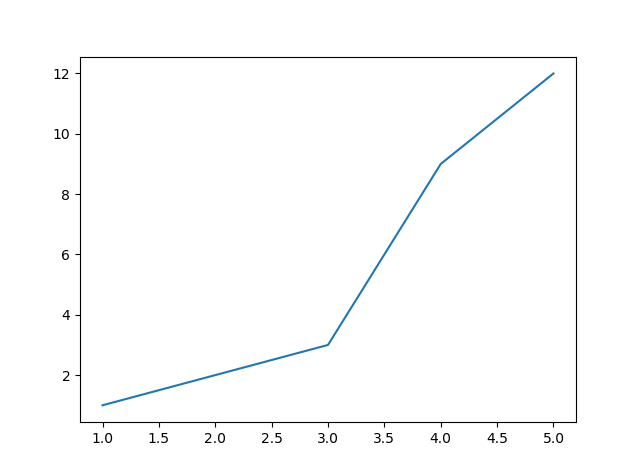
\includegraphics[width=\linewidth]{img/plt2.png}
    \caption{Črtni graf, pri čemer smo podali koordinate točk na obeh oseh.}
    \label{img:plt2}
\end{figure}
Na sliki je prikazan samo zadnji graf. Kam je izginil prejšnji? Kot smo že omenili knjižnica Matplotlib grafe riše na risalni površini v ozadju. Te prikaže, ko pokličemo funkcijo \texttt{show}, hkrati pa takrat risalno površino tudi počisti. Če hočemo na isti sliki prikazati več grafov, bomo pred klicanjem funkcije \texttt{show} pač narisali več grafov. Poskusimo to kar na zgledu s plačami, in sicer bi radi narisali podatke o povprečnih bruto plačah. Predpostavljali bomo, da smo funkcijo \texttt{uvozi\_place} shranili v program \texttt{place\_beri.py} in da se ta program nahaja v naši trenutni delovni mapi. Najprej bomo uvozili funkcijo za uvoz podatkov o plačah zraven pa še knjižnico Matplotlib:
\begin{lstlisting}[language=Python, showstringspaces=false]
>>> from place_beri import uvozi_place
>>> import matplotlib.pyplot as plt
\end{lstlisting}
Potem preberimo podatke o plačah:
\begin{lstlisting}[language=Python]
>>> place = uvozi_place('place.csv')
\end{lstlisting}
in potegnimo sezname is slovarjev:
\begin{lstlisting}[language=Python]
>>> MJ = place['Javni sektor']['mesec']
>>> ZJ = place['Javni sektor']['bruto']
>>> MZ = place['Zasebni sektor']['mesec']
>>> ZZ = place['Zasebni sektor']['bruto']
\end{lstlisting}
Zdaj bomo kot koordinate na osi $x$ podali podatke o mesecih, kot koordinate na osi $y$ pa podatke o zneskih in poklicali funkcijo za prikaz grafa. Takole:
\begin{lstlisting}[language=Python, showstringspaces=false]
>>> plt.plot(MJ, ZJ)
>>> plt.plot(MZ, ZZ)
>>> plt.show()
\end{lstlisting}
Več grafov lahko na isto sliko narišemo tudi tako, da naštejemo pare seznamov kar po vrsti. Takole: 
\begin{lstlisting}[language=Python, showstringspaces=false]
>>> plt.plot(MJ, ZJ, MZ, ZZ)
>>> plt.show()
\end{lstlisting}
Kljub temu, da je rezultat v zgornjih dveh primerih enak, bomo raje uporabljali prvi način.
Zapišimo zdaj vse skupaj kot program \texttt{risi\_place.py}.
\begin{lstlisting}[language=Python, showstringspaces=false,numbers=left]
from place_beri import uvozi_place # funkcija za uvoz
import matplotlib.pyplot as plt 
MJ, ZJ, MZ, ZZ = uvozi_place('place.csv')
plt.plot(MJ, ZJ) # riši javni sektor
plt.plot(MZ, ZZ) # riši zasebni sektor
plt.show() # prikaži graf
\end{lstlisting}
Rezultat izvedbe zgornjega programa prikazuje slika \ref{img:plt3}.
\begin{figure}
    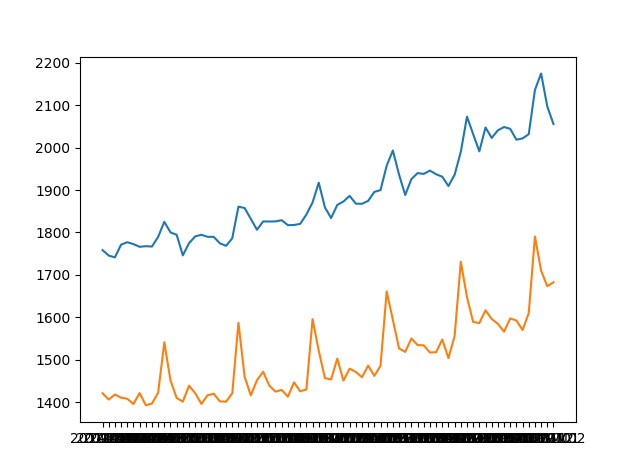
\includegraphics[width=\linewidth]{img/plt3.png}
    \caption{Osnovni izris podatkov o plačah.}
    \label{img:plt3}
\end{figure}

\section{Dodajanje oznak}
Vsak graf seveda potrebuje oznake. Označiti moramo kaj prikazuje posamezna os, za kar lahko uporabimo funkciji \texttt{xlabel} in \texttt{ylabel}, ki kot argument prejmeta niz, ki ga želimo prikazati. V našem primeru bi bilo smiselno napisati takole:
\begin{lstlisting}[language=Python, showstringspaces=false]
plt.xlabel("mesec")
plt.ylabel("znesek [EUR]")
\end{lstlisting}
Dodamo lahko tudi naslov grafa z uporabo funkcije \texttt{title}. Takole:
\begin{lstlisting}[language=Python, showstringspaces=false]
plt.title("Povprečne mesečne plače")
\end{lstlisting}

Manjka seveda tudi legenda. Kaj prikazuje modra linija in kaj oranžna? Legendo lahko dodamo tako, da oznake dodamo še posameznemu grafu kar med izrisom. Funkciji \texttt{plot} lahko preko opcijskega argumenta \texttt{label} podamo niz, ki predstavlja oznako grafa, ki ga bo izrisala. V našem primeru bi to naredili takole:
\begin{lstlisting}[language=Python, showstringspaces=false]
plt.plot(MJ, ZJ, label='Javni sektor') # riši javni sektor
plt.plot(MZ, ZZ, label='Zasebni sektor') # riši zasebni sektor
\end{lstlisting}
Če želimo legendo pokazati, moramo poklicati še funkcijo \texttt{legend}, ki prikaz legende vklopi:
\begin{lstlisting}[language=Python, showstringspaces=false]
plt.legend()
\end{lstlisting}
Vsebino legende, ki jo želimo izpisati bi lahko podali tudi neposredno funkciji \texttt{legend}. Takole:
\begin{lstlisting}[language=Python, showstringspaces=false]
plt.legend(['Javni sektor', 'Zasebni sektor'])
\end{lstlisting}
Pri tem moramo paziti na to, da oznake v legendi podajamo v enakem vrstnem redu, kot smo izvajali risanje grafov.


Zapišimo celoten program, ga poženimo in poglejmo rezultat. 
\begin{lstlisting}[language=Python, showstringspaces=false,numbers=left]
from place_beri import uvozi_place # funkcija za uvoz
import matplotlib.pyplot as plt

# uvozi podatke v slovar
place = uvozi_place('place.csv')
# pridobi sezname iz slovarja
MJ = place['Javni sektor']['mesec']
ZJ = place['Javni sektor']['bruto']
MZ = place['Zasebni sektor']['mesec']
ZZ = place['Zasebni sektor']['bruto']

plt.plot(MJ, ZJ) # riši javni sektor
plt.plot(MZ, ZZ) # riši zasebni sektor

# dodaj oznake
plt.xlabel("mesec")
plt.ylabel("znesek [EUR]")
plt.title("Povprečne mesečne plače")
plt.legend(['Javni sektor', 'Zasebni sektor'])

plt.show() # prikaži graf
\end{lstlisting}
Rezultat izvedbe zgornjega programa prikazuje slika \ref{img:plt4}.
\begin{figure}
    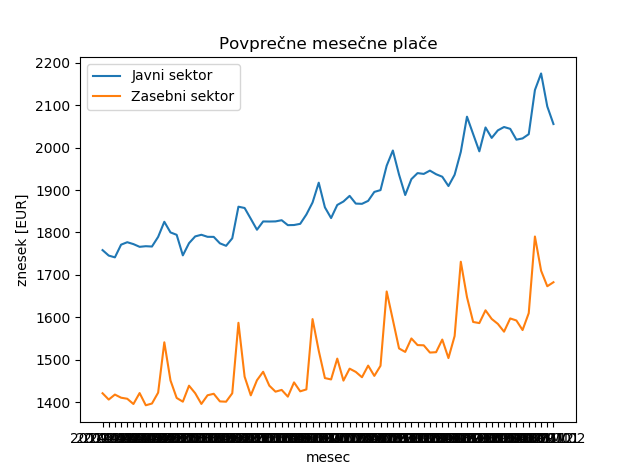
\includegraphics[width=\linewidth]{img/plt4.png}
    \caption{Izris podatkov o plačah z dodanimi oznakami.}
    \label{img:plt4}
\end{figure}

\section{Še malo prilagajanja oznak}
Kar nam še vedno ni všeč na sliki \ref{img:plt4} je neberljiv izpis na osi $x$. Če graf približamo, vidimo, da je na oseh izpisan podatek o mesecu. Mogoče bi bilo bolje, če bi ta podatek izpisali samo vsak januar, poleg tega pa bi informacijo o mesecu izpustili. Poskusimo odrezati rezino po mesecih od začetka do konca, pri čemer za korak nastavimo vrednost 12.
\begin{lstlisting}[language=Python, showstringspaces=false]
>>> MJ[::12]
['2014M01', '2015M01', '2016M01', '2017M01', '2018M01',
'2019M01', '2020M01']
\end{lstlisting}
Pripravimo si seznam \texttt{oznake}, ki bo vseboval samo podatke o letih. Vzeli bomo vsak 12-ti podatek iz obstoječega seznama mesecev (izhajamo lahko bodisi is seznama \texttt{MJ} ali \texttt{MZ}), pri čemer bomo upoštevali samo prve štiri znake (podatek o letu). 
\begin{lstlisting}[language=Python, showstringspaces=false]
oznake = []
for mj in MJ[::12]: # vzamemo vsako 12-to oznako
    oznake.append(mj[:4]) # vzamemo samo podatek o letu
\end{lstlisting}
Določiti moramo še lokacije, kjer bomo te oznake prikazali. Trenutno so oznake prikazane na lokacijah, ki se ujemajo z njihovimi indeksi, torej bi lahko lokacije oznak dobili s seznamoma \texttt{range(len(MJ))} ter \texttt{range(len(MZ))}. Ker bi radi prikazali vsako 12-to oznako, bomo morali torej upoštevati tudi vsako 12-to lokacijo. Takole:
\begin{lstlisting}[language=Python, showstringspaces=false]
# vsaka 12-ta lokacija
lokacije = range(0, len(MJ), 12) 
\end{lstlisting}

Lokacijo in vsebino oznak lahko zdaj našemu risarju podamo preko funkcije \texttt{xticks} (če bi želeli prilagajati oznake na osi $y$, bi uporabili funkcijo \texttt{yticks}):
\begin{lstlisting}[language=Python, showstringspaces=false]
plt.xticks(lokacije, oznake)
\end{lstlisting}

Celoten program je zdaj sledeč:
\begin{lstlisting}[language=Python, showstringspaces=false,numbers=left]
from place_beri import uvozi_place # funkcija za uvoz
import matplotlib.pyplot as plt

# uvozi podatke v slovar
place = uvozi_place('place.csv')
# pridobi sezname iz slovarja
MJ = place['Javni sektor']['mesec']
ZJ = place['Javni sektor']['bruto']
MZ = place['Zasebni sektor']['mesec']
ZZ = place['Zasebni sektor']['bruto']


# dodaj oznake
plt.xlabel("mesec")
plt.ylabel("znesek [EUR]")
plt.title("Povprečne mesečne plače")
plt.legend(['Javni sektor', 'Zasebni sektor'])

oznake = []
for mj in MJ[::12]: # vzamemo vsako 12-to oznako
    oznake.append(mj[:4]) # vzamemo samo podatek o letu

# vsaka 12-ta lokacija
lokacije = range(0, len(MJ), 12) 

plt.xticks(lokacije, oznake)

plt.show() # prikaži graf
\end{lstlisting}
Rezultat izvedbe programa prikazuje slika \ref{img:plt5}.
\begin{figure}
    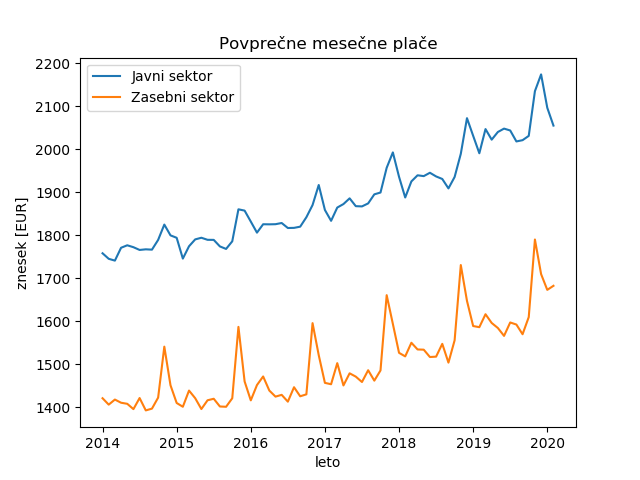
\includegraphics[width=\linewidth]{img/plt5.png}
    \caption{Izris podatkov o plačah s prilagojenimi oznakami na osi $x$.}
    \label{img:plt5}
\end{figure}

Kaj pa če bi imeli v podatkih o plačah še kakšen sektor več? Ker imamo podatke shranjene v dokaj prilagodljivi strukturi (slovarju), bi lahko izris naredili neodvisno od števila sektorjev. Enostavno se sprehodimo čez ključe slovarja in rišemo. Takole:
\begin{lstlisting}[language=Python]
for sektor in place:
    mesec = place[sektor]['mesec']
    znesek = place[sektor]['neto']
    plt.plot(mesec, znesek, label=sektor)
\end{lstlisting}
Tokrat smo oznake grafov dodajali že kar med izrisovanjem preko argumenta \texttt{label}. Pri risanju oznak na osi $x$ lahko uporabimo kar spremenljivko \texttt{mesec}, v kateri so ostali podatki zadnjega sektorja (po sprehodu z zanko \texttt{for}). Celotna koda je sledeča: 
\begin{lstlisting}[language=Python, showstringspaces=false,numbers=left]
from place_beri import uvozi_place # funkcija za uvoz
import matplotlib.pyplot as plt

# uvozi podatke v slovar
place = uvozi_place('place.csv')
# pridobi sezname iz slovarja
MJ = place['Javni sektor']['mesec']
ZJ = place['Javni sektor']['bruto']
MZ = place['Zasebni sektor']['mesec']
ZZ = place['Zasebni sektor']['bruto']


plt.plot(MJ, ZJ) # riši javni sektor
plt.plot(MZ, ZZ) # riši zasebni sektor

# dodaj oznake
plt.xlabel("mesec")
plt.ylabel("znesek [EUR]")
plt.title("Povprečne mesečne plače")
plt.legend(['Javni sektor', 'Zasebni sektor'])

oznake = []
for mj in MJ[::12]: # vzamemo vsako 12-to oznako
    oznake.append(mj[:4]) # vzamemo samo podatek o letu

# vsaka 12-ta lokacija
lokacije = range(0, len(MJ), 12) 

# prikaži oznake na osi x
plt.xticks(lokacije, oznake)

plt.show() # prikaži graf
\end{lstlisting}

\section{Ostale prilagoditve izrisa}
Če nam grafi še vedno niso všeč, se lahko igramo naprej. Preko funkcije \texttt{plot} lahko nastavljamo barvo izrisa (argument \texttt{color}), debelino črte (argument \texttt{linewidth}), tip črte (argument \texttt{linestyle}) in še marsikaj. Poleg tega lahko določamo razpon osi (funkcija \texttt{axis}), rišemo več podgrafov (funkcija \texttt{subplot}) in graf shranjujemo v datoteko (funkcija \texttt{savefig}). Možnosti je res veliko in jih tukaj ne bomo več naštevali. Primere različnih grafov, ki jih lahko izrišemo z uporabo knjižnice Matplotlib, si lahko bralec pogleda (in prosto dostopno kodo prilagodi za risanje svojih grafov) na povezavi \url{https://matplotlib.org/gallery}.

\section{Ostali tipi grafov}

Matplotlib poleg črtnega diagrama (funkcija \texttt{plot}) omogoča risanje tudi ostalih tipov grafov, npr. stolpičnega diagrama \angl{bar plot} s funkcijo \texttt{bar}, histograma s funkcijo \texttt{hist}, kvartilnega diagrama s funkcijo \texttt{box} itd. Poglejmo si še primer izrisa stolpičnega diagrama, pri čemer bomo prikazali podatke o povprečnih plačah za leto 2018. Najprej iz podatkov izluščimo zgolj podatke za leto 2018. Hkrati se bomo morali sprehajati čez mesece in zneske. Ker sta seznama poravnana (isti indeks se nanaša na isti mesec), lahko naredimo sprehod s pomočjo funkcije \texttt{zip}. Znotraj sprehoda pogledamo, če se mesec nanaša na leto 2018 in v tem primeru mesec in znesek dodamo v nova seznama, ki se nanašata na leto 2018. To naredimo za javni in zasebni sektor posebej:
\begin{lstlisting}[language=Python, showstringspaces=false]
# uvozi podatke v slovar
place = uvozi_place('place.csv')
# pridobi sezname iz slovarja
MJ = place['Javni sektor']['mesec']
ZJ = place['Javni sektor']['bruto']
MZ = place['Zasebni sektor']['mesec']
ZZ = place['Zasebni sektor']['bruto']

MJ_2018 = []
ZJ_2018 = []
MZ_2018 = []
ZZ_2018 = []

for mj, zj in zip(MJ, ZJ):
    if "2018" in mj:
        MJ_2018.append(mj)
        ZJ_2018.append(zj)

for mz, zz in zip(MZ, ZZ):
    if "2018" in mz:
        MZ_2018.append(mz)
        ZZ_2018.append(zz)
\end{lstlisting}

Zdaj lahko podatke narišemo, pri čemer bomo za izris uporabili funkcijo \texttt{bar}. Ena izmed razlik med funkcijo \texttt{bar} in \texttt{plot} je, da moramo pri prvi lokacije stolpcev na osi $x$ vedno podati. Uporabimo lahko kar funkcijo \texttt{range}:
\begin{lstlisting}[language=Python, showstringspaces=false]
plt.bar(range(len(ZJ_2018)), ZJ_2018)
plt.bar(range(len(ZZ_2018)), ZZ_2018)
\end{lstlisting}

Z uporabo funkcije \texttt{xticks} lahko določimo še oznake na osi $x$:
\begin{lstlisting}[language=Python, showstringspaces=false]
plt.xticks(range(len(MJ)), MJ)
\end{lstlisting}

Poglejmo si rezultat
\begin{lstlisting}[language=Python, showstringspaces=false]
plt.show()
\end{lstlisting}
Prikazuje ga slika \ref{img:plt6}.
\begin{figure}
    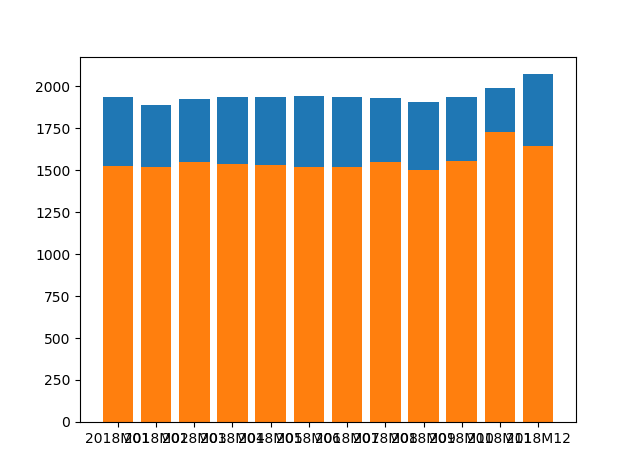
\includegraphics[width=\linewidth]{img/plt6.png}
    \caption{Izris podatkov o plačah za leto 2018 s stolpičnim diagramom.}
    \label{img:plt6}
\end{figure}
Oznake na osi $x$ so zopet moteči. Grafu bi lahko dodali naslov, da gre za leto 2018, na osi $x$ pa prikazali samo informacijo o mesecu. Tako bo postalo vse skupaj nekoliko bolj pregledno. Najprej iz oznak odstranimo podatek o letu. To lahko naredimo že med filtiranjem podatkov za leto 2018, kjer namesto stavkov \texttt{MJ\_2018.append(mj)} in \texttt{MZ\_2018.append(mz)} uporabimo stavka \texttt{MJ\_2018.append(mj[-3:])} in \texttt{MZ\_2018.append(mz[-3:])}. Naslov grafa dodamo s sledečo vrstico:
\begin{lstlisting}[language=Python, showstringspaces=false]
plt.title('Podatki o plačah za leto 2018')
\end{lstlisting}
Dodajmo še legendo:
\begin{lstlisting}[language=Python, showstringspaces=false]
plt.legend(['Javni sektor', 'Zasebni sektor'])
\end{lstlisting}

Celoten program je zdaj sledeč:
\begin{lstlisting}[language=Python, showstringspaces=false,numbers=left]
from place_beri import uvozi_place # funkcija za uvoz
import matplotlib.pyplot as plt

# uvozi podatke v slovar
place = uvozi_place('place.csv')
# pridobi sezname iz slovarja
MJ = place['Javni sektor']['mesec']
ZJ = place['Javni sektor']['bruto']
MZ = place['Zasebni sektor']['mesec']
ZZ = place['Zasebni sektor']['bruto']

# izluščimo podatke za leto 2018
MJ_2018 = []
ZJ_2018 = []
MZ_2018 = []
ZZ_2018 = []

for mj, zj in zip(MJ, ZJ):
    if "2018" in mj:
        MJ_2018.append(mj[-3:]) # brez leta
        ZJ_2018.append(zj)

for mz, zz in zip(MZ, ZZ):
    if "2018" in mz:
        MZ_2018.append(mz[-3:]) # brez leta
        ZZ_2018.append(zz)


plt.bar(range(len(ZJ_2018)), ZJ_2018)
plt.bar(range(len(ZZ_2018)), ZZ_2018)

plt.xticks(range(len(MJ_2018)), MJ_2018)

plt.title('Podatki o plačah za leto 2018')
plt.legend(['Javni sektor', 'Zasebni sektor'])
plt.show()
\end{lstlisting}
Rezultat izvedbe programa prikazuje slika \ref{img:plt7}.
\begin{figure}
    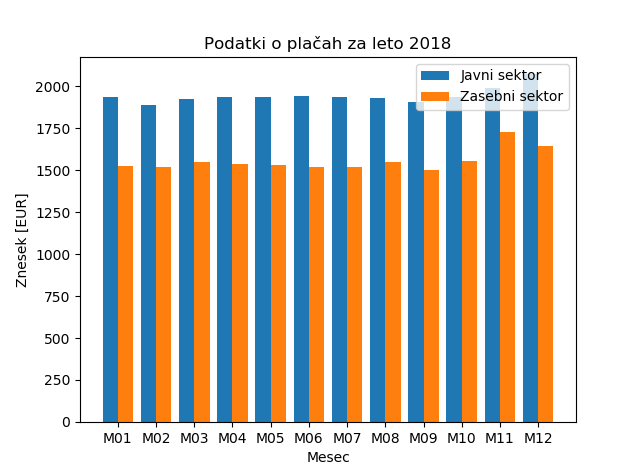
\includegraphics[width=\linewidth]{img/plt7.png}
    \caption{Dopolnjen in popravljen izris podatkov o plačah za leto 2018 s stolpičnim diagramom.}
    \label{img:plt7}
\end{figure}



\section{Risanje matematičnih funkcij}

\chapter{Knjižnica NumPy in hitro računanje}

\section{NumPy in struktura \texttt{ndarray}}

Knjižnica NumPy nadgrajuje Pythonove sezname, poleg tega pa nudi številne funkcije, ki nam olajšajo predvsem matematične operacije nad t.i. nadgrajenimi seznami oziroma strukturo \texttt{ndarray} \angl{N-dimensional array}. Vse se bo torej vrtelo okrog strukture \texttt{ndarray}. Kljub temu, da osnovna namestitev okolja Python knjižnice NumPy ne vsebuje, se je knjižnica namestila skupaj z namestitvijo knjižnice Matplotlib, saj jo slednji potrebuje za svoje delovanje. Uvozimo jo v svoje delovno okolje.
\begin{lstlisting}[language=Python]
>>> import numpy as np
\end{lstlisting}
Zdaj lahko poljuben seznam (ali seznamu podobno strukturo) pretvorimo v \texttt{ndarray} z uporabo funkcije \texttt{array}:
\begin{lstlisting}[language=Python]
>>> X = np.array([1,2,3])
>>> Y = np.array([4,5,6])
\end{lstlisting}
Kaj lahko z \emph{novimi} seznami počnemo? Podobno kot pri pri običajnih seznamih, lahko tudi te indeksiramo, nad njimi uporabljamo vgrajene funkcije, preverjamo, če vsebujejo določen element in se čez njih sprehajamo z zanko \texttt{for}:
\begin{lstlisting}[language=Python]
>>> X[0]
1
>>> len(X)
3
>>> 1 in X
True
>>> for x in X:
	print(x)
1
2
3
\end{lstlisting}

\section{Aritmetični operatorji in strutkura \texttt{ndarray}}

Sezname smo lahko med seboj tudi seštevali. Tudi \texttt{ndarray}-e lahko, vendar je rezultat nekoliko drugačen:
\begin{lstlisting}[language=Python]
>>> X+Y
array([5, 7, 9])
\end{lstlisting}
Dobili smo torej nov \texttt{ndarray}, ki je sestavljen iz vsote istoležnih elementov izhodiščnih \texttt{ndarray}-ev. Na tak \texttt{ndarray} lahko torej gledamo kot na vektor, na vsoto dveh \texttt{ndarray}-ev pa kot na vsoto dveh vektorjev. Zdaj je pogoj za seštevanje to, da sta oba vektorja oziroma \texttt{ndarray}-a enako dolga. Tole, npr. ne bo šlo:
\begin{lstlisting}[language=Python]
>>> Z = np.array([7,8])
>>> X+Z
ValueError: operands could not be broadcast together with shapes (3,) (2,) 
\end{lstlisting}
Lahko pa vektorju prištejemo skalar:
\begin{lstlisting}[language=Python]
>>> X+10
array([11, 12, 13]) 
\end{lstlisting}
Nad strukturami tipa \texttt{ndarray} lahko za razliko od seznamov uporabimo tudi druge aritmetične operatorje. Poskusimo:
\begin{lstlisting}[language=Python]
>>> X*Y
array([ 4, 10, 18])
>>> X/Y
array([0.25, 0.4 , 0.5 ])
>>> X-Y
array([-3, -3, -3])
>>> X**5
array([  1,  32, 243], dtype=int32)
>>> X/10
array([0.1, 0.2, 0.3])
\end{lstlisting}
Aritmetične operatorje lahko torej na tak način izvedemo nad vsakim elementom vektorja posebej. 

\section{Primerjalni operatorji, indeksiranje s seznami in filtiranje}

Podobno kot aritmetični delujejo nad strukturo  \texttt{ndarray} tudi primerjalni operatorji, in sicer tako, da primerjanje izvedejo nad vsakim elementom strukture posebej. Primerjamo lahko npr. dva vektorja:
\begin{lstlisting}[language=Python]
>>> X = np.array([1,2,3])
>>> Z = np.array([0.1, 10, -2])
>>> X < Z
array([False,  True, False])
\end{lstlisting}
Dobili smo torej vektor, ki vsebuje rezultate preverjanja na posameznih mestih. Primerjanje bi lahko izvajali tudi s skalarjem
\begin{lstlisting}[language=Python]
>>> X >= 2
array([False, True, True])
\end{lstlisting}

Dodatna prednost uporabe strukture \texttt{ndarray} je, da lahko to indeksiramo z vektorjem vrednosti \texttt{True} in \texttt{False}, pri čemer bomo kot rezultat dobili \texttt{ndarray} elementov, ki smo jih naslovili z vrednostjo \texttt{True}. Rezultat primerjanja strukture \texttt{ndarray} lahko torej uporabimo za indeksiranja. Če bi npr. želeli dobiti tiste elemente vektorja \texttt{X}, ki so večji ali enaki 2, bi lahko to naredili takole:
\begin{lstlisting}[language=Python]
>>> rez = X >= 2
>>> X[rez]
array([2, 3])
\end{lstlisting}
oziroma krajše:
\begin{lstlisting}[language=Python]
>>> X[X >= 2]
array([2, 3])
\end{lstlisting}
Tej operaciji lahko rečemo tudi \emph{filtriranje} vrednosti.

\section{Generiranje strukture \texttt{ndarray}}

Kot smo videli zgoraj lahko strukturo \texttt{ndarray} dobimo tako, da s funkcijo \texttt{array} vanjo pretvorimo običajen seznam. Modul NumPy pa ponuja tudi številne funkcije, ki jih lahko uporabimo pri generiranju  struktur \texttt{ndarray} z vnaprej poznanimi lastnostmi. Strukturo \texttt{ndarray}, ki npr. vsebuje same ničle, lahko zgeneriramo s funkcijo \texttt{zero}, same enice s funkcijo \texttt{ones}, matriko naključnih števil pa preko modula \texttt{numpy.random}. Podrobneje si bomo pogledali funkcijo \texttt{arange} in \texttt{linspace}, ki sta namenjeni generiranju struktur \texttt{ndarray} na vnaprej določenem intervalu.

Funkcija \texttt{arange} deluje zelo podobno kot funkcija \texttt{range}, le da vrača strukturo tipa \texttt{ndarray} poleg tega pa za razliko od funkcije \texttt{range} ni omejena na celoštevilske argumente. Če bi npr. želeli zgenerirati vektor vrednosti od 0.001 do 5 s korakom 0.001, bi to naredili s sledečim klicem:
\begin{lstlisting}[language=Python]
>>> X = np.arange(0.001, 5.001, 0.001)
\end{lstlisting}
Funkcija \texttt{linspace} deluje podobno, le da tej kot argumente podamo začetno in končno točko intervala (tokrat bo slednja v intervalu vsebovana) in število točk, ki jih želimo v intervalu imeti. Enak rezultat, kot ga dobimo z gornjim klicem funkcije \texttt{arange}, lahko dobimo tudi s funkcijo \texttt{linspace} takole:
\begin{lstlisting}[language=Python]
>>> X = np.linspace(0.001, 5, 5000)
\end{lstlisting}
Rekli smo torej, da želimo imeti 5000 točk na intervalu, ki se začne s točko 0.001 in konča s točko 5 (ta točka je v intervalu še vsebovana). Pri tem je uporabljena linearna interpolacija med točkami, kar z drugimi besedami pomeni, da od točke 0.001 do točke 5 potegnemo premico. 

\section{Funkcije nad strukturo \texttt{ndarray}}
Če želimo narisati graf logaritemske funkcije, lahko torej koordinate na osi $x$ enostavneje zgeneriramo s funkcijo \texttt{arange}. Zdaj moramo le še izračunati njihove logaritme. Poskusimo:
\begin{lstlisting}[language=Python]
>>> from math import log2, log, log10
>>> log2(X)
TypeError: only size-1 arrays can be converted to
Python scalars
\end{lstlisting}
Funkcije modula \texttt{math} torej nad vektorji ne moremo vektorsko izvajati, ampak se moramo spet zateči k zanki \texttt{for}. Izkaže pa se, da knjižnica NumPy poleg drugih vsebuje tudi matematične funkcije, ki zamenjuje tiste iz modula \texttt{math}, poleg tega pa podpirajo vektorski način izvajanja. Nad celotnim vektorjem jih torej lahko izvedemo z enim samim klicem. Poskusimo:
\begin{lstlisting}[language=Python]
>>> np.log2(X)
array([-9.96578428, -8.96578428, -8.38082178, ...,
2.3213509 , 2.32163953,  2.32192809])
\end{lstlisting}

Zdaj lahko dokončamo zgled z risanjem logaritemskih funkcij.

\begin{zgled}
Nariši grafe logaritemskih funkcij z osnovo 2, $\textrm{e}$ in 10 na intervalu od 0 do 5. Sliko opremi z legendami, vsak graf pa naj bo narisan s svojo barvo.
\end{zgled}

\begin{resitev}
Rešitev bo zdaj bistveno krajša, saj bomo vrednosti na osi $x$ generirali s funkcijo \texttt{np.arange} (ena vrstica), logaritme pa računali s funkcijami \texttt{np.log2}, \texttt{np.log} in \texttt{np.log10} (tri vrstice). Ostala koda bo ostala enaka, prav tako pa bo enak rezultat, ki je prikazan na sliki \ref{img:plt9}.
\begin{lstlisting}[language=Python,numbers=left]
import numpy as np
import matplotlib.pyplot as plt

# hitro generiranje vrednosti na osi x
X = np.arange(0.001, 5.001, 0.001) 

# računanje logaritmov brez zanke for 
Y_2 = np.log2(X)
Y_e = np.log(X)
Y_10 = np.log10(X)

# nespremenjena koda od prej
plt.plot(X,Y_2, label="$log_2(x)$")
plt.plot(X,Y_e, label="$log_e(x)$")
plt.plot(X,Y_10, label="$log_{10}(x)$")
plt.xlabel('x')
plt.ylabel('y')
plt.legend()

plt.show()
\end{lstlisting}
\end{resitev}

\section{Več dimenzij}

Tekom spoznavanja seznamov smo se srečali tudi s seznami seznamov oziroma z ugnezdenimi seznami. Primer takega seznama je sledeč:
\begin{lstlisting}[language=Python]
>>> sez = [[1, 2, 3], [4, 5, 6], [7, 8, 9]]
\end{lstlisting}
Kaj se zgodi, če tak seznam pretvorimo v strukturo \texttt{ndarray}:
\begin{lstlisting}[language=Python]
>>> A = np.array(sez)
>>> A
array([[1, 2, 3],
       [4, 5, 6],
       [7, 8, 9]])
\end{lstlisting}
Na prvi pogled nič kaj presenetljivega, ampak če smo lahko na strukturo \texttt{ndarray}, ki smo jo dobili iz navadnega seznama gledali na vektor, lahko na strukturo \texttt{ndarray}, ki jo dobimo iz ugnezdenih seznamov gledamo na matriko oziroma na dvodimenzionalno strukturo, ki ima podatke zapisane v vrsticah (dimenzija 0) in stolpcih (dimenzija 1). Indeksiramo jo lahko tako kot običajne ugnezdene sezname. Do ugnezdenega podseznama na npr. indeksu 1, lahko pridemo takole:
\begin{lstlisting}[language=Python]
>>> A[1]
array([4, 5, 6])
\end{lstlisting}
V matrični interpretaciji to predstavlja vrstico 1 matrike z imenom \texttt{1}. Do elementa na indeksu 2 vrstice 1 lahko torej pridemo takole:
\begin{lstlisting}[language=Python]
>>> A[1][2]
6
\end{lstlisting}
Delovanje je bilo do tukaj zelo podobno kot pri običajnih ugnezdenih seznamih, le interpretacija je malo drugačna. Enako bi lahko naredili tudi pri običajnem seznamu
\begin{lstlisting}[language=Python]
>>> sez[1][2]
6
\end{lstlisting}
Pri delu s strukturo \texttt{ndarray} lahko do elementov matrike pridemo tudi tako, da znotraj oglatih oklepajev podamo indeks vrstice in indeks stolpca. To pri običajnih seznamih ne gre:
\begin{lstlisting}[language=Python]
>>> A[1,2]
6
>>> sez[1,2]
TypeError: list indices must be integers or slices, 
not tuple
\end{lstlisting}
Pri indeksiranju smo torej najprej podali indeks po ničti dimenziji oziroma indeks vrstice, potem pa indeks po prvi dimenziji oziroma indeks stolpca (nič nas ne omejuje pri tem, da ne bi število dimenzij še povečali -- tako bi dobili tenzor). Tako dobljene matrike lahko podobno kot vektorje med seboj tudi npr. seštevamo in jim prištevamo skalarje:
\begin{lstlisting}[language=Python]
>>> B = np.array([[10, 11, 12], 
                  [-1, -2, -3], 
                  [0.1, 0.2, 0.3]])
>>> A+B
array([[11. , 13. , 15. ],
       [ 3. ,  3. ,  3. ],
       [ 7.1,  8.2,  9.3]])
\end{lstlisting}
Nad njimi lahko delamo tudi rezine, in sicer preko vsake dimenzije posebej. Če bi želeli npr. iz matrike \texttt{A} dobiti vrstice od 0 do 2, in stolpce od 1 do konca, bi to napisali takole:
\begin{lstlisting}[language=Python]
>>> A[:2,1:]
array([[2, 3],
       [5, 6]])
\end{lstlisting}
Lahko bi dobili tudi specifično vrstico. Vrstico 2, bi npr. dobili takole:
\begin{lstlisting}[language=Python]
>>> A[2,:]
array([7, 8, 9])
\end{lstlisting}
Kaj smo s tem povedali? Rekli smo, da želimo ničto dimenzijo fiksirati na indeks 2 (vrstica številka 2), dimenzijo 1 pa želimo imeti v celoti (vsi stolpci). To bi lahko sicer napisali tudi takole
\begin{lstlisting}[language=Python]
>>> A[2]
array([7, 8, 9])
\end{lstlisting}
in bi seveda delovalo tudi nad navadnimi seznami. Kako bi lahko prišli do specifičnega stolpca? Podobno kot prej, le da zdaj fiksiramo indeks stolpca in se sprehajamo čez vse vrstice. Do stolpca številka 2 bi torej prišli takole:
\begin{lstlisting}[language=Python]
>>> A[:,2]
array([3, 6, 9])
\end{lstlisting}
Tega nad običajnimi seznami ne moremo (tako enostavno) narediti.


\section{Ostale uporabne funkcije}
Knjižnica NumPy ponuja še vrsto drugih uporabnih funkcij, ki pa jih boste spoznali, če boste knjižnico bolj intenzivno uporabljali. Nekaj jih bomo vseeno omenili.

Za izračun vsote elementov, določitev minimalnega in maksimalnega lahko uporabimo vgrajene funkcije \texttt{min}, \texttt{max} in \texttt{sum}. Te funkcije pa odpovejo, ko ima naša struktura več dimenzij ali pa vsebuje posebne vrednosti (glej razdelek \ref{sec:np_nan}). V tem primeru lahko uporabljamo funkcije modula NumPy, tj. \texttt{np.min}, \texttt{np.max} in \texttt{np.sum}. V osnovi te funkcije delujejo nad celotno strukturo, kar pomeni. Takole:
\begin{lstlisting}[language=Python]
>>> A = np.array([[1,2,3],[4,5,6],[7,8,9]])
>>> np.min(A)
1
>>> np.max(A)
9
>>> np.sum(A)
45
\end{lstlisting}
Včasih želimo določeno operacijo izvesti le nad npr. vrsticami ali stolpci matrike. V tem primeru lahko pri uporabi zgornjih funkcij podamo še vrednost izbirnega argumenta \texttt{axis}. Če ta argument nastavimo na vrednost 0, se bomo tekom operacije znebili dimenzije 0 (vrstic), kar pomeni, da bomo dobili rezultat izvedbe operacije po stolpcih.
\begin{lstlisting}[language=Python]
>>> A = np.array([[1,2,3],[4,5,6],[7,8,9]])
>>> np.min(A, axis=0)
array([1, 2, 3])
>>> np.max(A, axis=0)
array([7, 8, 9])
>>> np.sum(A, axis=0)
array([12, 15, 18])
\end{lstlisting}
Če argument \texttt{axis} nastavimo na vrednost 1, se bomo s tem znebili dimenzije 1 (stolpcev), kar pomeni, da bomo operacijo izvedli po vrsticah:
\begin{lstlisting}[language=Python]
>>> A = np.array([[1,2,3],[4,5,6],[7,8,9]])
>>> np.min(A, axis=1)
array([1, 4, 7])
>>> np.max(A, axis=1)
array([3, 6, 9])
>>> np.sum(A, axis=1)
array([ 6, 15, 24])
\end{lstlisting}

\section{Posebne vrednosti}
\label{sec:np_nan}

Knjižnica NumPy omogoča, da kot števila predstavimo tudi posebne vrednosti. Prava tako vrednost je uporabna predvsem v primerih, ko nam določen podatek manjka. Če npr. beležimo višino, telesno maso in starost oseb, se lahko hitro zgodi, da med podatki kakšen manjka. Narobe bi bilo, če bi tak podatek postavili na neko običajno numerično vrednost (npr. 0), saj bi nam to pokvarilo določene statistike, kot je npr. povprečje. Prav tako velikokrat podatka ne moremo kar izpustiti. Če želimo podatke npr. beležiti v matriki tipa \texttt{ndarray}, morajo imeti vse vrstice enako število stolpcev. V tem primeru lahko uporabimo posebno vrednost \texttt{np.nan} \angl{not a number}, ki predstavlja t.i. \emph{placeholder} in drži prazno mesto, hkrati pa ga lahko pri analizi vrednosti obravnavamo drugače kot ostale vrednosti (npr. ga izpustimo). V primeru, da naši podatki lahko vsebujejo vrednost \texttt{np.nan} in želimo to pri analizah ignorirati, lahko namesto funkcijo kot so \texttt{np.min}, \texttt{np.max} in \texttt{np.sum} uporabimo funkcije \texttt{np.nanmin}, \texttt{np.nanmax} in \texttt{np.nansum}.

Poleg vrednosti \texttt{np.nan} knjižnica NumPy vsebuje tudi posebno vrednost \texttt{np.inf}, s katero lahko npr. zapišemo rezultat deljenja z nič ali pa logaritem števila 0. Pri tem sicer dobimo opozorilo (ne pa napake):
\begin{lstlisting}[language=Python]
>>> np.log(0)
RuntimeWarning: divide by zero encountered in log
-inf
\end{lstlisting}

\section{Uvažanje vrednosti in omejitve strukture \texttt{ndarray}}

V prejšnjih poglavjih smo že omenili datoteke CSV. Ker se taka oblika zapisovanja pogosto uporablja tudi za numerične podatke, knjižnica NumPy podpira uvoz tovrstnih datotek preko funkcij \texttt{np.genfromtxt} in \texttt{np.loadtxt}. Kadar datoteka vsebuje zgolj numerične podatke (števila) funkciji ustvarita enak rezultat, in sicer vrneta strukturo \texttt{ndarray} z vsebino datoteke. Pri tem funkcijama kot argument \texttt{encoding} podamo kodiranje datoteke kot argument \texttt{delimiter} pa ločilo, ki je uporabljeno znotraj datoteke.

Naj ima datoteka z imenom \texttt{stevila1.csv} sledečo vsebino:
\begin{lstlisting}[numbers=left]
180.3,87.3
161.5,77.3
170,56.5
156,55.3
\end{lstlisting}
Preberemo jo lahko takole:
\begin{lstlisting}[language=Python]
>>> A1 = np.genfromtxt("stevila1.csv",
                       encoding="utf-8", delimiter=",")
>>> B1 = np.loadtxt("stevila1.csv", 
                    encoding="utf-8", 
                    delimiter=",")
\end{lstlisting}

Pri tem v obeh primerih dobimo enak rezultat:
\begin{lstlisting}[language=Python]
>>> A1
array([[180.3,  87.3],
       [161.5,  77.3],
       [170. ,  56.5],
       [156. ,  55.3]])
>>> B1
array([[180.3,  87.3],
       [161.5,  77.3],
       [170. ,  56.5],
       [156. ,  55.3]])
\end{lstlisting}
Do težav pride, kadar datoteka vsebuje tudi podatke, ki niso številskega tipa. Ena izmed glavnih omejitev strukture \texttt{ndarray} je namreč ta, da zahteva, da vsi njeni podatki pripadajo enakemu podatkovnemu tipu. Podatkovni tip strukture lahko preverimo preko atributa (atribut je spremenljivka, ki pripada določenemu objektu -- podobno kot je metoda funkcija, ki pripada določenemu objektu) \texttt{dtype}.  
\begin{lstlisting}[numbers=left]
>>> A1.dtype # do atributov dostopamo brez oklepajev
dtype('float64')
\end{lstlisting}
Vsi podatki v strukturi \texttt{A1} so torej decimalna števila. 

Kaj se torej zgodi, če datoteka vsebuje podatke, ki niso števila. Dopolnimo našo datoteko s stolpcem, ki bo vsebovala imena ljudi, ki seveda niso števila. To shranimo v datoteko {stevila2.csv}:
\begin{lstlisting}[numbers=left]
Janez,180.3,87.3
Andrej,161.5,77.3
Ana,170,56.5
Katja,156,55.3
\end{lstlisting}

Funkcija \texttt{np.genfromtxt} bo imena enostavno pretvorila v vrednosti \texttt{np.nan}, saj to lahko zapiše kot število. S tem bo dobljena struktura še vedno lahko vsebovala števila, s katerimi bomo lahko računali. Poskusimo:
\begin{lstlisting}[language=Python]
>>> A2 = np.genfromtxt("stevila2.csv",
                       encoding="utf-8",
                       delimiter=",")
>>> A2
array([[  nan, 180.3,  87.3],
       [  nan, 161.5,  77.3],
       [  nan, 170. ,  56.5],
       [  nan, 156. ,  55.3]])
\end{lstlisting}
S tem smo informacijo o imenih sicer izgubili, smo pa ohranili podatkovni tip strukture, tako da ta še vedno vsebuje števila
\begin{lstlisting}[language=Python]
>>> A2.dtype
dtype('float64')
\end{lstlisting}
Kaj pa funkcija  \texttt{np.loadtxt}? Ta poskuša na vsak način podatke pretvoriti v števila, zato ob odpiranju take datoteke vrne napako:
\begin{lstlisting}[language=Python]
>>> B2 = np.loadtxt("stevila2.csv", 
                    encoding="utf-8", 
                    delimiter=",")
ValueError: could not convert string to float: 'Janez'
\end{lstlisting}
Lahko jo nekoliko prelisičimo, da ji naročimo, naj datoteko uvozi kot nize. To naredimo preko opcijskega argumenta \texttt{dtype}, ki ga nastavimo na vrednost \texttt{str} ali pa vrednost \texttt{'U'} \angl{Unicode string}. 
\begin{lstlisting}[language=Python]
>>> B2 = np.loadtxt("stevila2.csv", 
                    encoding="utf-8", 
                    delimiter=",", 
                    dtype=str)
array([['Janez', '180.3', '87.3'],
       ['Andrej', '161.5', '77.3'],
       ['Ana', '170', '56.5'],
       ['Katja', '156', '55.3']], dtype='<U6')
\end{lstlisting}
Zdaj smo podatke uspešno uvozili, ampak za ceno tega, da z njimi ne moremo več računati. Če bi želeli do numeričnih vrednosti vseeno priti, lahko odvržemo stolpec 0, ostale vrednosti pa pretvorimo v števila. Takole:
\begin{lstlisting}[language=Python]
>>> B2[:,1:].astype(float)
array([[180.3,  87.3],
       [161.5,  77.3],
       [170. ,  56.5],
       [156. ,  55.3]]))
\end{lstlisting}
Opomba: funkcija \texttt{astype} izhodiščne strukture ne spreminja, ampak vrne spremenjeno strukturo.

Datoteka bi lahko vsebovala tudi imena stolpcev. V našem primeru bi to izgledalo nekako takole (datoteka {stevila3.csv}:
\begin{lstlisting}[numbers=left]
ime,višina,teža
Janez,180.3,87.3
Andrej,161.5,77.3
Ana,170,56.5
Katja,156,55.3
\end{lstlisting} 
V tem primeru lahko funkciji \texttt{np.genfromtxt} naročimo, naj ločeno uvozi imena stolpcev preko izbirnega argumenta \texttt{names}, ki ga nastavimo na vrednost \texttt{True}:
\begin{lstlisting}[language=Python]
>>> A3 = np.genfromtxt("stevila3.csv",
                       encoding="utf-8",
                       delimiter=",", 
                       names=True)
\end{lstlisting}
Zdaj so imena stolpcev zapisana ločeno znotraj atributa \texttt{dtype}.
\begin{lstlisting}[language=Python]
>>> A3
array([(nan, 180.3, 87.3), (nan, 161.5, 77.3), (nan, 170. , 56.5),
       (nan, 156. , 55.3)],
      dtype=[('ime', '<f8'), ('višina', '<f8'), ('teža', '<f8')])
>>> A3.dtype.names
('ime', 'višina', 'teža')
\end{lstlisting}
Do imen stolpcev torej lahko pridemo, je pa malo nerodno. Pri uporabi funkcije \texttt{np.loadtxt} bi lahko postopali podobno kot prej in celotno datoteko uvozili kot \texttt{ndarray} nizov:
\begin{lstlisting}[language=Python]
>>> B3 = np.loadtxt("stevila3.csv", encoding="utf-8", delimiter=",", dtype='U')
>>> B3
array([['ime', 'višina', 'teža'],
       ['Janez', '180.3', '87.3'],
       ['Andrej', '161.5', '77.3'],
       ['Ana', '170', '56.5'],
       ['Katja', '156', '55.3']], dtype='<U6')
\end{lstlisting}
S tem se seveda spet odpovemo zmožnostim računanja, saj se z nizi pač računati ne da. 

\section{Primernost knjižnice NumPy}

Knjižnica NumPy je torej idealna za delo z numeričnimi podatki. Do problema pa pride, kadar naši podatki poleg numeričnih vrednosti vsebujejo tudi nize, ki jih ne moremo obravnavati kot števila. To so lahko zgolj imena stolpcev ali pa tudi drugi podatki. Pri plačah smo se npr. srečali s podatki o mesecu, v zgornjih primerih pa s podatki o imeni osebe. Ko pridemo do takih podatkov moramo skleniti kompromis. Lahko se jim odpovemo z njihovo pretvorbo v \texttt{np.nan}, kar ponavadi ne pride v upoštev. Lahko vse podatke zapišemo v obliki nizov, s čimer se odpovemo zmožnostim računanja. Možna alternativa je tudi, da numerične podatke shranimo v drugo strukturo kot nenumerične. To nam načeloma povzroči dodatno delo, je pa seveda izvedljivo. V vsakem primeru so komplikacije neizogibne. Lahko pa v takem primeru uporabimo knjižnico Pandas, ki je namenjena delu z večjimi količinami podatkov.







%\begin{appendices}
%\appendixpage
%\include{slovarcek}
%\end{appendices}
%\chapter*{Vaje x}
%\section*{Avditorne vaje}
%\section*{Laboratorijske vaje}

%\backmatter

%%% BIBLIOGRAPHY
%%% -------------------------------------------------------------

%\bibliographystyle{plain}
%\bibliography{reference}

\end{document}

